\documentclass[a4paper,12pt]{article}

\usepackage[margin=2.5cm]{geometry}
\usepackage[T1]{fontenc}
\usepackage[utf8]{inputenc}
\usepackage{lmodern}
\usepackage{amsmath,amssymb,amsthm}
\usepackage{booktabs}
\usepackage{xcolor}
\usepackage{hyperref}
\usepackage{tikz}
\usetikzlibrary{arrows.meta,positioning,calc,shapes.geometric,fit,decorations.pathmorphing,decorations.pathreplacing}

\hypersetup{
  colorlinks=true,
  linkcolor=blue!50!black,
  citecolor=blue!50!black,
  urlcolor=blue!50!black
}

\newtheorem{definition}{Definition}
\newtheorem{remark}{Remark}
\newtheorem{proposition}{Proposition}

\title{\textbf{Optimizing an Explicit Unit-Distance Lower-Bound Certificate}}
\author{Michael T. M. Emmerich\thanks{Faculty of Information Technology, University of Jyv\"askyl\"a, Finland. ORCID: \href{https://orcid.org/0000-0002-7342-2090}{0000-0002-7342-2090}.}}
\date{May 30, 2026}

\begin{document}
\maketitle

\begin{abstract}
The 2026 disproof of Erd\H{o}s's unit-distance conjecture and Sawin's subsequent explicit quantitative refinement show that the maximum number $u(n)$ of unit distances among $n$ planar points can exceed $n^{1+\varepsilon}$ for a fixed positive $\varepsilon$.  Sawin's explicit bound gives more than $n^{1.014}$ unit distances for arbitrarily large $n$ and exposes finite parameters whose choice is not fully optimized.  This report formulates a reproducible optimization framework for these parameters and records a verification pipeline that is first validated by reproducing Sawin's published parameter choice and then applied to an optimized candidate.  The main computational contribution is a finite search and checking procedure for the sets of primes $T$ and $S_Q$, the multiplicities $k(p)$, and the parameter $R$.  On Sawin's published example the same pipeline reproduces the stated exponent $\delta\approx 0.0141144$, which serves as a validation test before the improved candidate is considered.  The best candidate studied here satisfies the implemented arithmetic checks, exactly saturates the relevant Golod--Shafarevich budget, and gives the numerical exponent gain
\[
\delta=0.01517180563721325\ldots .
\]
Consequently, subject to the explicit criterion of Sawin being applied exactly as cited, the candidate supports the cautious clean statement $u(n)>n^{1.015}$ for arbitrarily large $n$.  The report also includes an explicit finite planar comparator, based on the classical multi-direction lattice construction with squared length 5, to illustrate a genuine coordinate realization that improves on the ordinary square-grid unit-distance graph while remaining distinct from the optimized certificate.
\end{abstract}

\noindent\textbf{Keywords.} Erd\H{o}s unit-distance problem; discrete geometry; algebraic number theory; Golod--Shafarevich inequality; class-field towers; mixed-integer nonlinear optimization; reproducible verification.

\medskip

\noindent\textbf{MSC 2020.} 52C10; 11R29; 11R37; 90C11; 90C59.

\section{Introduction}

For a finite point set $P\subset\mathbb{R}^2$, let
\[
  U(P)=\#\bigl\{\{x,y\}\subset P:\|x-y\|=1\bigr\},
\]
and define
\[
  u(n)=\max_{|P|=n} U(P).
\]
The classical unit-distance problem asks for the asymptotic growth of $u(n)$.  Erd\H{o}s conjectured that lattice-type constructions are essentially optimal, in the sense that $u(n)$ should be bounded by $n^{1+o(1)}$ \cite{Erdos1946,OpenAI2026}.  The best general upper bounds remain much larger, of order $O(n^{4/3})$, through incidence-geometric methods related to the Szemer\'edi--Trotter theorem \cite{ST1983,SST1984}.

In 2026, OpenAI announced a counterexample to the Erd\H{o}s conjecture, and a human-verified exposition by Alon, Bloom, Gowers, Litt, Sawin, Shankar, Tsimerman, Wang, and Matchett Wood described the structure of the argument and its relation to earlier number-theoretic ideas \cite{OpenAI2026,AlonEtAl2026}.  Sawin then gave an explicit quantitative refinement, proving that there are arbitrarily large $n$-point sets with more than $n^{1.014}$ unit-distance pairs \cite{Sawin2026}.

The purpose of this note is narrower than reproving the counterexample.  It studies the finite parameter-selection problem exposed by Sawin's explicit criterion, with an emphasis on reproducible computation and internal validation against the published explicit example.  The main contributions are:
\begin{enumerate}
  \item an optimization formulation for choosing the finite data $(T,S_Q,k,R)$;
  \item a reproducible verification pipeline for checking a candidate against the relevant arithmetic side conditions implemented here, together with a validation run reproducing Sawin's published $n^{1.014\ldots}$ example;
  \item a cautiously stated candidate improvement of the clean explicit exponent from $1.014$ to $1.015$, conditional on Sawin's criterion being applied exactly as cited;
  \item a clear separation between certificate verification and the substantially harder problem of constructing actual planar coordinates.
\end{enumerate}
No claim is made here that a coordinate realization of the optimized candidate has been generated.

\section{Optimization framework}

The explicit lower-bound criterion suggests the following finite parameter-selection problem.  One chooses:
\begin{itemize}
  \item a finite set $T$ of odd primes;
  \item a finite set $S_Q$ of rational primes;
  \item integer multiplicities $k(p)\geq 1$ for $p\in S_Q$;
  \item a real parameter $R>1$.
\end{itemize}

For the implementation discussed below, define
\[
  e(p)=
  \begin{cases}
  2, & p=2\text{ or }p\in T,\\
  1, & \text{otherwise.}
  \end{cases}
\]
The exponent-gain objective used in the verification is
\begin{align}
\delta(T,S_Q,k,R)&=\frac{N(T,S_Q,k,R)}{D(T,S_Q,k,R)},\label{eq:delta-objective}\\
N(T,S_Q,k,R)&=\log(1-1/R)+\frac12\log(2\pi/e)\notag\\
&\quad+\sum_{p\in S_Q}\frac{1}{4e(p)}\log(k(p)+1)
-\frac18\log\!\left(4\prod_{q\in T}q\right)\notag\\
&\quad-\frac12\log\!\log\!\sqrt{4\prod_{q\in T}q},\notag\\
D(T,S_Q,k,R)&=\log\!\left(2R\prod_{p\in S_Q}p^{k(p)/(2e(p))}+1\right).\notag
\end{align}
The resulting optimization problem is to maximize $\delta(T,S_Q,k,R)$ subject to arithmetic side conditions.  The search stage uses a lightweight admissibility model to generate candidates; the candidate reported in Appendix~\ref{app:verification} is then checked separately by exact integer arithmetic for the side conditions implemented in the verification pipeline.

\section{Heuristic budget and greedy score}

One useful side condition has the form
\[
  \#T+\#S_Q+\#\{p\in S_Q:p\text{ splits in }Q\}+1
  \leq \frac{(\#T-1)^2}{4},
\]
where $Q=\mathbb{Q}\!\left(\sqrt{\prod_{q\in T}q}\right)$ in the simplified quadratic-field picture.  This suggests viewing the construction of $S_Q$ as a knapsack-like problem: a non-splitting prime costs one unit of budget, while a splitting prime costs two.

For a provisional target exponent $c$, a first-order rule gives
\[
  k(p)\approx \left\lfloor \frac{1}{2c\log p}-1\right\rfloor,
  \qquad
  R\approx 1+\frac{1}{c}.
\]
The implemented script ranks admissible primes by the score
\[
  \operatorname{score}(p)=
  \frac{\frac{1}{4e(p)}\log(k(p)+1)}{\operatorname{cost}(p)},
\]
then greedily fills the available budget.  This gives a finite mixed-integer nonlinear optimization problem with number-theoretic feasibility constraints.

\section{Visualization}

This section collects figures that clarify the geometric meaning of the unit-distance relation and the status of the various planar drawings used later in the paper.

Figure~\ref{fig:optimization-flow} shows the optimization loop used to generate candidate certificates.  The solid arrows show the main parameter path.  The dashed frame marks the greedy subproblem in which candidate primes are scored and selected.

\begin{figure}[htbp]
\centering
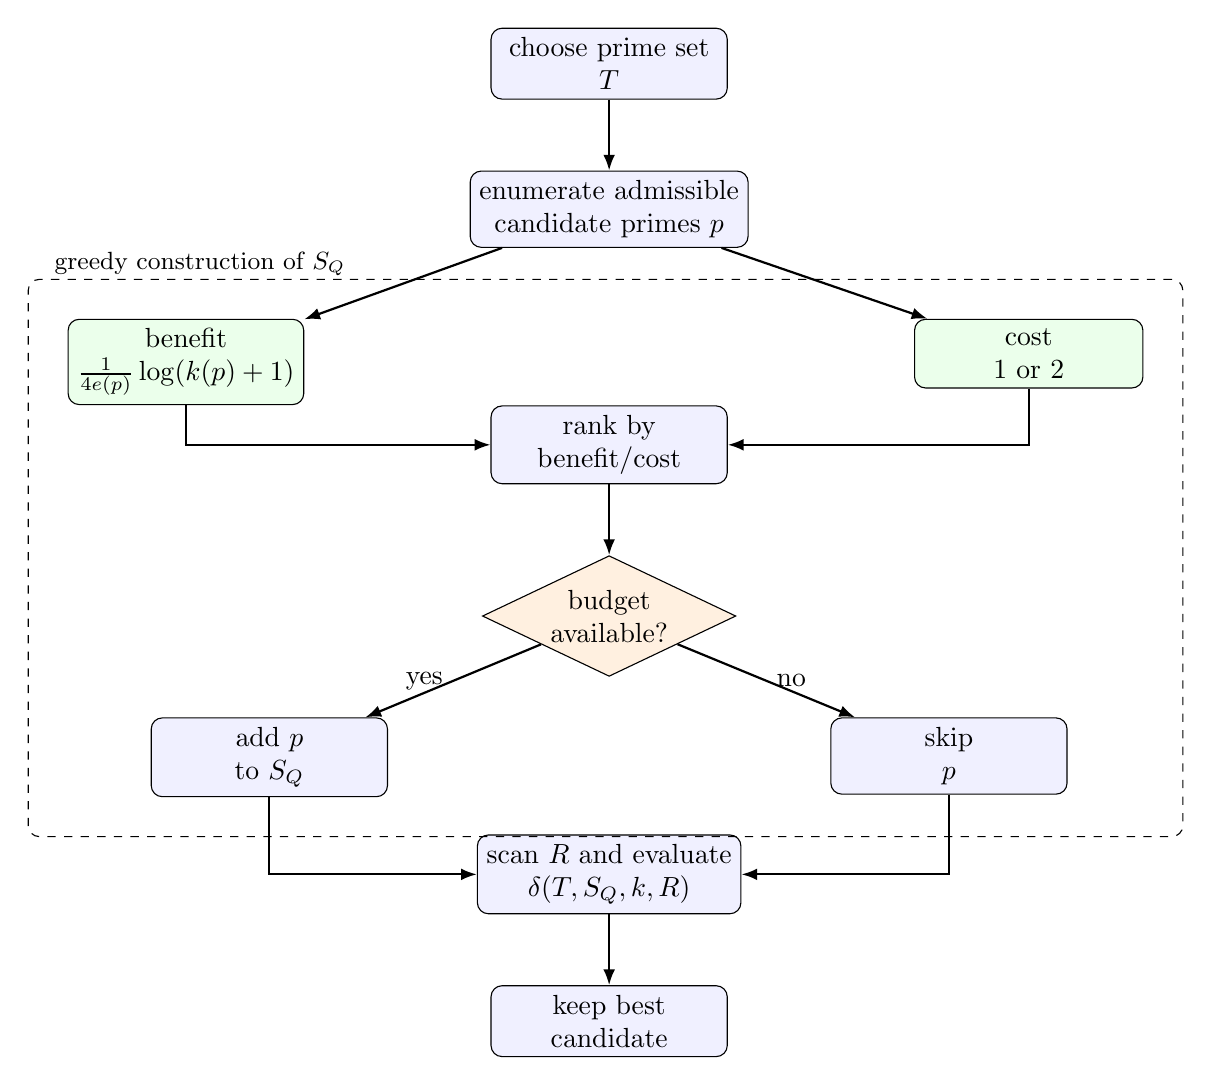
\begin{tikzpicture}[
  node distance=9mm and 9mm,
  box/.style={draw, rounded corners, align=center, minimum height=9mm, minimum width=30mm, fill=blue!6},
  smallbox/.style={draw, rounded corners, align=center, minimum height=8mm, minimum width=29mm, fill=green!8},
  decision/.style={draw, diamond, aspect=2.1, align=center, fill=orange!12, inner sep=1.5pt},
  line/.style={-{Latex[length=2mm]}, thick},
  softline/.style={-{Latex[length=2mm]}, thick, dashed, color=gray!70!black}
]

\node[box] (T) {choose prime set\\$T$};
\node[box, below=of T] (candidates) {enumerate admissible\\candidate primes $p$};
\node[smallbox, below left=of candidates, xshift=-12mm] (benefit) {benefit\\$\frac{1}{4e(p)}\log(k(p)+1)$};
\node[smallbox, below right=of candidates, xshift=12mm] (cost) {cost\\$1$ or $2$};
\node[box, below=20mm of candidates] (score) {rank by\\benefit/cost};
\node[decision, below=of score] (budget) {budget\\available?};
\node[box, below left=of budget, xshift=-11mm] (add) {add $p$\\to $S_Q$};
\node[box, below right=of budget, xshift=11mm] (skip) {skip\\$p$};
\node[box, below=20mm of budget] (scanR) {scan $R$ and evaluate\\$\delta(T,S_Q,k,R)$};
\node[box, below=of scanR] (best) {keep best\\candidate};

\draw[line] (T) -- (candidates);
\draw[line] (candidates) -- (benefit);
\draw[line] (candidates) -- (cost);
\draw[line] (benefit) |- (score);
\draw[line] (cost) |- (score);
\draw[line] (score) -- (budget);
\draw[line] (budget) -- node[left] {yes} (add);
\draw[line] (budget) -- node[right] {no} (skip);
\draw[line] (add.south) |- (scanR.west);
\draw[line] (skip.south) |- (scanR.east);
\draw[line] (scanR) -- (best);

\node[draw, dashed, rounded corners, fit=(benefit)(cost)(score)(budget)(add)(skip), inner sep=5mm] (greedybox) {};
\node[anchor=south west, font=\small, fill=white, inner sep=1pt] at ([xshift=3mm]greedybox.north west) {greedy construction of $S_Q$};
\end{tikzpicture}
\caption{A conceptual optimization pattern for selecting $(T,S_Q,k,R)$.}
\label{fig:optimization-flow}
\end{figure}

\subsection{A planar unit-disk contact patch}

Figure~\ref{fig:unit-disk-contact-patch} is a purely geometric patch included to recall the unit-distance relation.  It shows a hexagonal unit-disk contact pattern clipped to the square $[-10,10]^2$.  The disks have radius $1$ and transparent interiors with solid boundaries; two centers are connected precisely when the corresponding disks touch, i.e. when their center distance is $2$.  Rescaling all coordinates by a factor $1/2$ converts this into a unit-distance graph picture.

\begin{figure}[htbp]
\centering
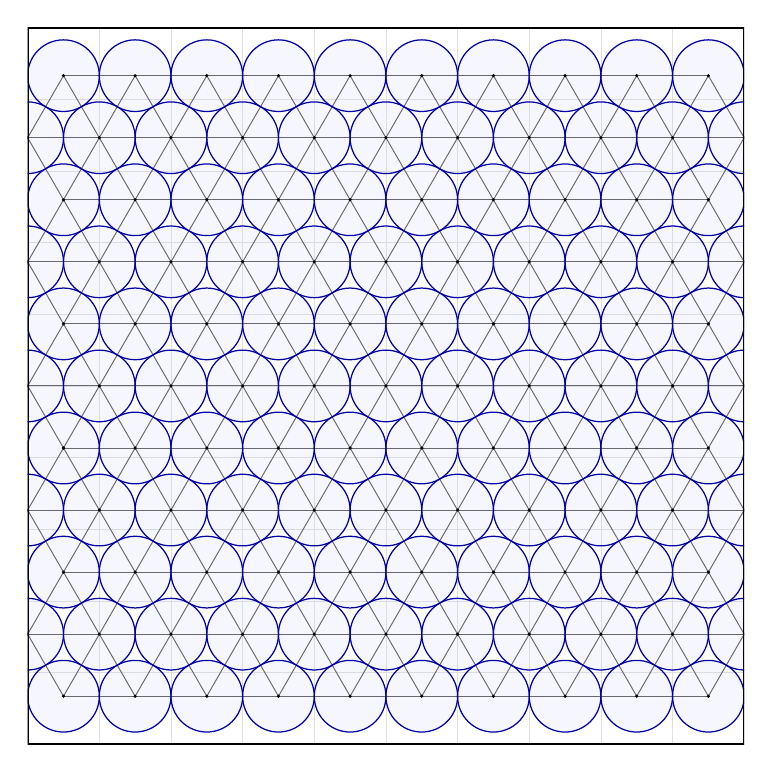
\begin{tikzpicture}[
  scale=0.455,
  contact/.style={draw=gray!65!black, line width=0.35pt},
  disk/.style={draw=blue!65!black, fill=blue!20, fill opacity=0.18, line width=0.45pt},
  center/.style={circle, fill=black, inner sep=0.45pt},
  boundary/.style={draw=black, line width=0.7pt},
  gridline/.style={draw=gray!25, line width=0.2pt}
]
  % Work inside the requested window.
  \clip (-10,-10) rectangle (10,10);

  % Light coordinate grid for the square [-10,10]^2.
  \foreach \g in {-10,-8,...,10} {
    \draw[gridline] (\g,-10) -- (\g,10);
    \draw[gridline] (-10,\g) -- (10,\g);
  }

  % Contact edges: centers are joined exactly when the unit disks touch.
  \draw[contact] (-9,-8.660) -- (-7,-8.660);
  \draw[contact] (-9,-8.660) -- (-10,-6.928);
  \draw[contact] (-9,-8.660) -- (-8,-6.928);
  \draw[contact] (-7,-8.660) -- (-5,-8.660);
  \draw[contact] (-7,-8.660) -- (-8,-6.928);
  \draw[contact] (-7,-8.660) -- (-6,-6.928);
  \draw[contact] (-5,-8.660) -- (-3,-8.660);
  \draw[contact] (-5,-8.660) -- (-6,-6.928);
  \draw[contact] (-5,-8.660) -- (-4,-6.928);
  \draw[contact] (-3,-8.660) -- (-1,-8.660);
  \draw[contact] (-3,-8.660) -- (-4,-6.928);
  \draw[contact] (-3,-8.660) -- (-2,-6.928);
  \draw[contact] (-1,-8.660) -- (1,-8.660);
  \draw[contact] (-1,-8.660) -- (-2,-6.928);
  \draw[contact] (-1,-8.660) -- (0,-6.928);
  \draw[contact] (1,-8.660) -- (3,-8.660);
  \draw[contact] (1,-8.660) -- (0,-6.928);
  \draw[contact] (1,-8.660) -- (2,-6.928);
  \draw[contact] (3,-8.660) -- (5,-8.660);
  \draw[contact] (3,-8.660) -- (2,-6.928);
  \draw[contact] (3,-8.660) -- (4,-6.928);
  \draw[contact] (5,-8.660) -- (7,-8.660);
  \draw[contact] (5,-8.660) -- (4,-6.928);
  \draw[contact] (5,-8.660) -- (6,-6.928);
  \draw[contact] (7,-8.660) -- (9,-8.660);
  \draw[contact] (7,-8.660) -- (6,-6.928);
  \draw[contact] (7,-8.660) -- (8,-6.928);
  \draw[contact] (9,-8.660) -- (8,-6.928);
  \draw[contact] (9,-8.660) -- (10,-6.928);
  \draw[contact] (-10,-6.928) -- (-8,-6.928);
  \draw[contact] (-10,-6.928) -- (-9,-5.196);
  \draw[contact] (-8,-6.928) -- (-6,-6.928);
  \draw[contact] (-8,-6.928) -- (-9,-5.196);
  \draw[contact] (-8,-6.928) -- (-7,-5.196);
  \draw[contact] (-6,-6.928) -- (-4,-6.928);
  \draw[contact] (-6,-6.928) -- (-7,-5.196);
  \draw[contact] (-6,-6.928) -- (-5,-5.196);
  \draw[contact] (-4,-6.928) -- (-2,-6.928);
  \draw[contact] (-4,-6.928) -- (-5,-5.196);
  \draw[contact] (-4,-6.928) -- (-3,-5.196);
  \draw[contact] (-2,-6.928) -- (0,-6.928);
  \draw[contact] (-2,-6.928) -- (-3,-5.196);
  \draw[contact] (-2,-6.928) -- (-1,-5.196);
  \draw[contact] (0,-6.928) -- (2,-6.928);
  \draw[contact] (0,-6.928) -- (-1,-5.196);
  \draw[contact] (0,-6.928) -- (1,-5.196);
  \draw[contact] (2,-6.928) -- (4,-6.928);
  \draw[contact] (2,-6.928) -- (1,-5.196);
  \draw[contact] (2,-6.928) -- (3,-5.196);
  \draw[contact] (4,-6.928) -- (6,-6.928);
  \draw[contact] (4,-6.928) -- (3,-5.196);
  \draw[contact] (4,-6.928) -- (5,-5.196);
  \draw[contact] (6,-6.928) -- (8,-6.928);
  \draw[contact] (6,-6.928) -- (5,-5.196);
  \draw[contact] (6,-6.928) -- (7,-5.196);
  \draw[contact] (8,-6.928) -- (10,-6.928);
  \draw[contact] (8,-6.928) -- (7,-5.196);
  \draw[contact] (8,-6.928) -- (9,-5.196);
  \draw[contact] (10,-6.928) -- (9,-5.196);
  \draw[contact] (-9,-5.196) -- (-7,-5.196);
  \draw[contact] (-9,-5.196) -- (-10,-3.464);
  \draw[contact] (-9,-5.196) -- (-8,-3.464);
  \draw[contact] (-7,-5.196) -- (-5,-5.196);
  \draw[contact] (-7,-5.196) -- (-8,-3.464);
  \draw[contact] (-7,-5.196) -- (-6,-3.464);
  \draw[contact] (-5,-5.196) -- (-3,-5.196);
  \draw[contact] (-5,-5.196) -- (-6,-3.464);
  \draw[contact] (-5,-5.196) -- (-4,-3.464);
  \draw[contact] (-3,-5.196) -- (-1,-5.196);
  \draw[contact] (-3,-5.196) -- (-4,-3.464);
  \draw[contact] (-3,-5.196) -- (-2,-3.464);
  \draw[contact] (-1,-5.196) -- (1,-5.196);
  \draw[contact] (-1,-5.196) -- (-2,-3.464);
  \draw[contact] (-1,-5.196) -- (0,-3.464);
  \draw[contact] (1,-5.196) -- (3,-5.196);
  \draw[contact] (1,-5.196) -- (0,-3.464);
  \draw[contact] (1,-5.196) -- (2,-3.464);
  \draw[contact] (3,-5.196) -- (5,-5.196);
  \draw[contact] (3,-5.196) -- (2,-3.464);
  \draw[contact] (3,-5.196) -- (4,-3.464);
  \draw[contact] (5,-5.196) -- (7,-5.196);
  \draw[contact] (5,-5.196) -- (4,-3.464);
  \draw[contact] (5,-5.196) -- (6,-3.464);
  \draw[contact] (7,-5.196) -- (9,-5.196);
  \draw[contact] (7,-5.196) -- (6,-3.464);
  \draw[contact] (7,-5.196) -- (8,-3.464);
  \draw[contact] (9,-5.196) -- (8,-3.464);
  \draw[contact] (9,-5.196) -- (10,-3.464);
  \draw[contact] (-10,-3.464) -- (-8,-3.464);
  \draw[contact] (-10,-3.464) -- (-9,-1.732);
  \draw[contact] (-8,-3.464) -- (-6,-3.464);
  \draw[contact] (-8,-3.464) -- (-9,-1.732);
  \draw[contact] (-8,-3.464) -- (-7,-1.732);
  \draw[contact] (-6,-3.464) -- (-4,-3.464);
  \draw[contact] (-6,-3.464) -- (-7,-1.732);
  \draw[contact] (-6,-3.464) -- (-5,-1.732);
  \draw[contact] (-4,-3.464) -- (-2,-3.464);
  \draw[contact] (-4,-3.464) -- (-5,-1.732);
  \draw[contact] (-4,-3.464) -- (-3,-1.732);
  \draw[contact] (-2,-3.464) -- (0,-3.464);
  \draw[contact] (-2,-3.464) -- (-3,-1.732);
  \draw[contact] (-2,-3.464) -- (-1,-1.732);
  \draw[contact] (0,-3.464) -- (2,-3.464);
  \draw[contact] (0,-3.464) -- (-1,-1.732);
  \draw[contact] (0,-3.464) -- (1,-1.732);
  \draw[contact] (2,-3.464) -- (4,-3.464);
  \draw[contact] (2,-3.464) -- (1,-1.732);
  \draw[contact] (2,-3.464) -- (3,-1.732);
  \draw[contact] (4,-3.464) -- (6,-3.464);
  \draw[contact] (4,-3.464) -- (3,-1.732);
  \draw[contact] (4,-3.464) -- (5,-1.732);
  \draw[contact] (6,-3.464) -- (8,-3.464);
  \draw[contact] (6,-3.464) -- (5,-1.732);
  \draw[contact] (6,-3.464) -- (7,-1.732);
  \draw[contact] (8,-3.464) -- (10,-3.464);
  \draw[contact] (8,-3.464) -- (7,-1.732);
  \draw[contact] (8,-3.464) -- (9,-1.732);
  \draw[contact] (10,-3.464) -- (9,-1.732);
  \draw[contact] (-9,-1.732) -- (-7,-1.732);
  \draw[contact] (-9,-1.732) -- (-10,0);
  \draw[contact] (-9,-1.732) -- (-8,0);
  \draw[contact] (-7,-1.732) -- (-5,-1.732);
  \draw[contact] (-7,-1.732) -- (-8,0);
  \draw[contact] (-7,-1.732) -- (-6,0);
  \draw[contact] (-5,-1.732) -- (-3,-1.732);
  \draw[contact] (-5,-1.732) -- (-6,0);
  \draw[contact] (-5,-1.732) -- (-4,0);
  \draw[contact] (-3,-1.732) -- (-1,-1.732);
  \draw[contact] (-3,-1.732) -- (-4,0);
  \draw[contact] (-3,-1.732) -- (-2,0);
  \draw[contact] (-1,-1.732) -- (1,-1.732);
  \draw[contact] (-1,-1.732) -- (-2,0);
  \draw[contact] (-1,-1.732) -- (0,0);
  \draw[contact] (1,-1.732) -- (3,-1.732);
  \draw[contact] (1,-1.732) -- (0,0);
  \draw[contact] (1,-1.732) -- (2,0);
  \draw[contact] (3,-1.732) -- (5,-1.732);
  \draw[contact] (3,-1.732) -- (2,0);
  \draw[contact] (3,-1.732) -- (4,0);
  \draw[contact] (5,-1.732) -- (7,-1.732);
  \draw[contact] (5,-1.732) -- (4,0);
  \draw[contact] (5,-1.732) -- (6,0);
  \draw[contact] (7,-1.732) -- (9,-1.732);
  \draw[contact] (7,-1.732) -- (6,0);
  \draw[contact] (7,-1.732) -- (8,0);
  \draw[contact] (9,-1.732) -- (8,0);
  \draw[contact] (9,-1.732) -- (10,0);
  \draw[contact] (-10,0) -- (-8,0);
  \draw[contact] (-10,0) -- (-9,1.732);
  \draw[contact] (-8,0) -- (-6,0);
  \draw[contact] (-8,0) -- (-9,1.732);
  \draw[contact] (-8,0) -- (-7,1.732);
  \draw[contact] (-6,0) -- (-4,0);
  \draw[contact] (-6,0) -- (-7,1.732);
  \draw[contact] (-6,0) -- (-5,1.732);
  \draw[contact] (-4,0) -- (-2,0);
  \draw[contact] (-4,0) -- (-5,1.732);
  \draw[contact] (-4,0) -- (-3,1.732);
  \draw[contact] (-2,0) -- (0,0);
  \draw[contact] (-2,0) -- (-3,1.732);
  \draw[contact] (-2,0) -- (-1,1.732);
  \draw[contact] (0,0) -- (2,0);
  \draw[contact] (0,0) -- (-1,1.732);
  \draw[contact] (0,0) -- (1,1.732);
  \draw[contact] (2,0) -- (4,0);
  \draw[contact] (2,0) -- (1,1.732);
  \draw[contact] (2,0) -- (3,1.732);
  \draw[contact] (4,0) -- (6,0);
  \draw[contact] (4,0) -- (3,1.732);
  \draw[contact] (4,0) -- (5,1.732);
  \draw[contact] (6,0) -- (8,0);
  \draw[contact] (6,0) -- (5,1.732);
  \draw[contact] (6,0) -- (7,1.732);
  \draw[contact] (8,0) -- (10,0);
  \draw[contact] (8,0) -- (7,1.732);
  \draw[contact] (8,0) -- (9,1.732);
  \draw[contact] (10,0) -- (9,1.732);
  \draw[contact] (-9,1.732) -- (-7,1.732);
  \draw[contact] (-9,1.732) -- (-10,3.464);
  \draw[contact] (-9,1.732) -- (-8,3.464);
  \draw[contact] (-7,1.732) -- (-5,1.732);
  \draw[contact] (-7,1.732) -- (-8,3.464);
  \draw[contact] (-7,1.732) -- (-6,3.464);
  \draw[contact] (-5,1.732) -- (-3,1.732);
  \draw[contact] (-5,1.732) -- (-6,3.464);
  \draw[contact] (-5,1.732) -- (-4,3.464);
  \draw[contact] (-3,1.732) -- (-1,1.732);
  \draw[contact] (-3,1.732) -- (-4,3.464);
  \draw[contact] (-3,1.732) -- (-2,3.464);
  \draw[contact] (-1,1.732) -- (1,1.732);
  \draw[contact] (-1,1.732) -- (-2,3.464);
  \draw[contact] (-1,1.732) -- (0,3.464);
  \draw[contact] (1,1.732) -- (3,1.732);
  \draw[contact] (1,1.732) -- (0,3.464);
  \draw[contact] (1,1.732) -- (2,3.464);
  \draw[contact] (3,1.732) -- (5,1.732);
  \draw[contact] (3,1.732) -- (2,3.464);
  \draw[contact] (3,1.732) -- (4,3.464);
  \draw[contact] (5,1.732) -- (7,1.732);
  \draw[contact] (5,1.732) -- (4,3.464);
  \draw[contact] (5,1.732) -- (6,3.464);
  \draw[contact] (7,1.732) -- (9,1.732);
  \draw[contact] (7,1.732) -- (6,3.464);
  \draw[contact] (7,1.732) -- (8,3.464);
  \draw[contact] (9,1.732) -- (8,3.464);
  \draw[contact] (9,1.732) -- (10,3.464);
  \draw[contact] (-10,3.464) -- (-8,3.464);
  \draw[contact] (-10,3.464) -- (-9,5.196);
  \draw[contact] (-8,3.464) -- (-6,3.464);
  \draw[contact] (-8,3.464) -- (-9,5.196);
  \draw[contact] (-8,3.464) -- (-7,5.196);
  \draw[contact] (-6,3.464) -- (-4,3.464);
  \draw[contact] (-6,3.464) -- (-7,5.196);
  \draw[contact] (-6,3.464) -- (-5,5.196);
  \draw[contact] (-4,3.464) -- (-2,3.464);
  \draw[contact] (-4,3.464) -- (-5,5.196);
  \draw[contact] (-4,3.464) -- (-3,5.196);
  \draw[contact] (-2,3.464) -- (0,3.464);
  \draw[contact] (-2,3.464) -- (-3,5.196);
  \draw[contact] (-2,3.464) -- (-1,5.196);
  \draw[contact] (0,3.464) -- (2,3.464);
  \draw[contact] (0,3.464) -- (-1,5.196);
  \draw[contact] (0,3.464) -- (1,5.196);
  \draw[contact] (2,3.464) -- (4,3.464);
  \draw[contact] (2,3.464) -- (1,5.196);
  \draw[contact] (2,3.464) -- (3,5.196);
  \draw[contact] (4,3.464) -- (6,3.464);
  \draw[contact] (4,3.464) -- (3,5.196);
  \draw[contact] (4,3.464) -- (5,5.196);
  \draw[contact] (6,3.464) -- (8,3.464);
  \draw[contact] (6,3.464) -- (5,5.196);
  \draw[contact] (6,3.464) -- (7,5.196);
  \draw[contact] (8,3.464) -- (10,3.464);
  \draw[contact] (8,3.464) -- (7,5.196);
  \draw[contact] (8,3.464) -- (9,5.196);
  \draw[contact] (10,3.464) -- (9,5.196);
  \draw[contact] (-9,5.196) -- (-7,5.196);
  \draw[contact] (-9,5.196) -- (-10,6.928);
  \draw[contact] (-9,5.196) -- (-8,6.928);
  \draw[contact] (-7,5.196) -- (-5,5.196);
  \draw[contact] (-7,5.196) -- (-8,6.928);
  \draw[contact] (-7,5.196) -- (-6,6.928);
  \draw[contact] (-5,5.196) -- (-3,5.196);
  \draw[contact] (-5,5.196) -- (-6,6.928);
  \draw[contact] (-5,5.196) -- (-4,6.928);
  \draw[contact] (-3,5.196) -- (-1,5.196);
  \draw[contact] (-3,5.196) -- (-4,6.928);
  \draw[contact] (-3,5.196) -- (-2,6.928);
  \draw[contact] (-1,5.196) -- (1,5.196);
  \draw[contact] (-1,5.196) -- (-2,6.928);
  \draw[contact] (-1,5.196) -- (0,6.928);
  \draw[contact] (1,5.196) -- (3,5.196);
  \draw[contact] (1,5.196) -- (0,6.928);
  \draw[contact] (1,5.196) -- (2,6.928);
  \draw[contact] (3,5.196) -- (5,5.196);
  \draw[contact] (3,5.196) -- (2,6.928);
  \draw[contact] (3,5.196) -- (4,6.928);
  \draw[contact] (5,5.196) -- (7,5.196);
  \draw[contact] (5,5.196) -- (4,6.928);
  \draw[contact] (5,5.196) -- (6,6.928);
  \draw[contact] (7,5.196) -- (9,5.196);
  \draw[contact] (7,5.196) -- (6,6.928);
  \draw[contact] (7,5.196) -- (8,6.928);
  \draw[contact] (9,5.196) -- (8,6.928);
  \draw[contact] (9,5.196) -- (10,6.928);
  \draw[contact] (-10,6.928) -- (-8,6.928);
  \draw[contact] (-10,6.928) -- (-9,8.660);
  \draw[contact] (-8,6.928) -- (-6,6.928);
  \draw[contact] (-8,6.928) -- (-9,8.660);
  \draw[contact] (-8,6.928) -- (-7,8.660);
  \draw[contact] (-6,6.928) -- (-4,6.928);
  \draw[contact] (-6,6.928) -- (-7,8.660);
  \draw[contact] (-6,6.928) -- (-5,8.660);
  \draw[contact] (-4,6.928) -- (-2,6.928);
  \draw[contact] (-4,6.928) -- (-5,8.660);
  \draw[contact] (-4,6.928) -- (-3,8.660);
  \draw[contact] (-2,6.928) -- (0,6.928);
  \draw[contact] (-2,6.928) -- (-3,8.660);
  \draw[contact] (-2,6.928) -- (-1,8.660);
  \draw[contact] (0,6.928) -- (2,6.928);
  \draw[contact] (0,6.928) -- (-1,8.660);
  \draw[contact] (0,6.928) -- (1,8.660);
  \draw[contact] (2,6.928) -- (4,6.928);
  \draw[contact] (2,6.928) -- (1,8.660);
  \draw[contact] (2,6.928) -- (3,8.660);
  \draw[contact] (4,6.928) -- (6,6.928);
  \draw[contact] (4,6.928) -- (3,8.660);
  \draw[contact] (4,6.928) -- (5,8.660);
  \draw[contact] (6,6.928) -- (8,6.928);
  \draw[contact] (6,6.928) -- (5,8.660);
  \draw[contact] (6,6.928) -- (7,8.660);
  \draw[contact] (8,6.928) -- (10,6.928);
  \draw[contact] (8,6.928) -- (7,8.660);
  \draw[contact] (8,6.928) -- (9,8.660);
  \draw[contact] (10,6.928) -- (9,8.660);
  \draw[contact] (-9,8.660) -- (-7,8.660);
  \draw[contact] (-7,8.660) -- (-5,8.660);
  \draw[contact] (-5,8.660) -- (-3,8.660);
  \draw[contact] (-3,8.660) -- (-1,8.660);
  \draw[contact] (-1,8.660) -- (1,8.660);
  \draw[contact] (1,8.660) -- (3,8.660);
  \draw[contact] (3,8.660) -- (5,8.660);
  \draw[contact] (5,8.660) -- (7,8.660);
  \draw[contact] (7,8.660) -- (9,8.660);

  % Transparent unit disks with solid boundaries.
  \foreach \x/\y in {
    -9/-8.660,
    -7/-8.660,
    -5/-8.660,
    -3/-8.660,
    -1/-8.660,
    1/-8.660,
    3/-8.660,
    5/-8.660,
    7/-8.660,
    9/-8.660,
    -10/-6.928,
    -8/-6.928,
    -6/-6.928,
    -4/-6.928,
    -2/-6.928,
    0/-6.928,
    2/-6.928,
    4/-6.928,
    6/-6.928,
    8/-6.928,
    10/-6.928,
    -9/-5.196,
    -7/-5.196,
    -5/-5.196,
    -3/-5.196,
    -1/-5.196,
    1/-5.196,
    3/-5.196,
    5/-5.196,
    7/-5.196,
    9/-5.196,
    -10/-3.464,
    -8/-3.464,
    -6/-3.464,
    -4/-3.464,
    -2/-3.464,
    0/-3.464,
    2/-3.464,
    4/-3.464,
    6/-3.464,
    8/-3.464,
    10/-3.464,
    -9/-1.732,
    -7/-1.732,
    -5/-1.732,
    -3/-1.732,
    -1/-1.732,
    1/-1.732,
    3/-1.732,
    5/-1.732,
    7/-1.732,
    9/-1.732,
    -10/0,
    -8/0,
    -6/0,
    -4/0,
    -2/0,
    0/0,
    2/0,
    4/0,
    6/0,
    8/0,
    10/0,
    -9/1.732,
    -7/1.732,
    -5/1.732,
    -3/1.732,
    -1/1.732,
    1/1.732,
    3/1.732,
    5/1.732,
    7/1.732,
    9/1.732,
    -10/3.464,
    -8/3.464,
    -6/3.464,
    -4/3.464,
    -2/3.464,
    0/3.464,
    2/3.464,
    4/3.464,
    6/3.464,
    8/3.464,
    10/3.464,
    -9/5.196,
    -7/5.196,
    -5/5.196,
    -3/5.196,
    -1/5.196,
    1/5.196,
    3/5.196,
    5/5.196,
    7/5.196,
    9/5.196,
    -10/6.928,
    -8/6.928,
    -6/6.928,
    -4/6.928,
    -2/6.928,
    0/6.928,
    2/6.928,
    4/6.928,
    6/6.928,
    8/6.928,
    10/6.928,
    -9/8.660,
    -7/8.660,
    -5/8.660,
    -3/8.660,
    -1/8.660,
    1/8.660,
    3/8.660,
    5/8.660,
    7/8.660,
    9/8.660
  } {
    \filldraw[disk] (\x,\y) circle (1);
    \node[center] at (\x,\y) {};
  }

  % Boundary of the visible square.
  \draw[boundary] (-10,-10) rectangle (10,10);
\end{tikzpicture}
\caption{A unit-disk contact patch in the square $[-10,10]^2$.  The disks have radius $1$; edges connect centers of touching disks, so each edge has length $2$ before rescaling.}
\label{fig:unit-disk-contact-patch}
\end{figure}



\subsection{A local example illustrating touching, overlap, and separation}\label{subsec:touch-overlap-separate}

The unit-distance problem is not a packing problem, and it is useful to separate three different geometric relations.  If disks of radius $1/2$ are centered at the points of a planar set, then two disks are tangent precisely when their centers are at distance $1$.  However, the problem does not require all other disks to be disjoint.  In particular, one may simultaneously have point pairs at distance $1$ (the edges of the unit-distance graph), point pairs at distance strictly less than $1$ (hence overlapping half-unit disks), and point pairs at distance greater than $1$ (hence separated half-unit disks).  Figure~\ref{fig:touch-overlap-separate} records these three possibilities in a single local example.

\begin{figure}[htbp]
\centering
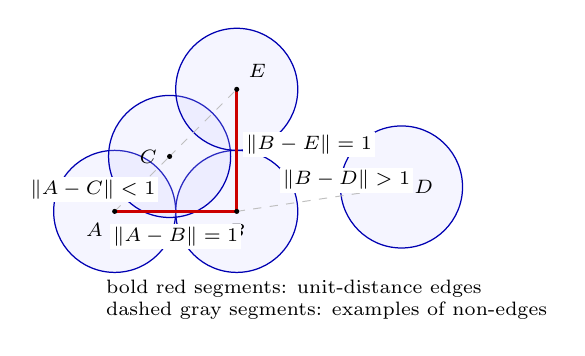
\begin{tikzpicture}[
  scale=1.55,
  halfdisk/.style={draw=blue!70!black, fill=blue!20, fill opacity=0.20, line width=0.45pt},
  unitedge/.style={draw=red!80!black, line width=1.0pt},
  pt/.style={circle, fill=black, inner sep=0.65pt},
  faint/.style={draw=gray!50, dashed, line width=0.35pt},
  lab/.style={font=\scriptsize, fill=white, inner sep=1pt}
]
  % points
  \coordinate (A) at (0,0);
  \coordinate (B) at (1,0);
  \coordinate (E) at (1,1);
  \coordinate (C) at (0.45,0.45);
  \coordinate (D) at (2.35,0.20);

  % half-unit disks
  \foreach \P in {A,B,C,D,E} {
    \draw[halfdisk] (\P) circle[radius=0.5];
  }

  % unit-distance edges in bold red
  \draw[unitedge] (A) -- (B);
  \draw[unitedge] (B) -- (E);

  % optional guide segments for one overlap and one separated pair
  \draw[faint] (A) -- (C);
  \draw[faint] (C) -- (E);
  \draw[faint] (B) -- (D);

  % points and labels
  \node[pt,label=below left:{\scriptsize $A$}] at (A) {};
  \node[pt,label=below:{\scriptsize $B$}] at (B) {};
  \node[pt,label=above right:{\scriptsize $E$}] at (E) {};
  \node[pt,label=left:{\scriptsize $C$}] at (C) {};
  \node[pt,label=right:{\scriptsize $D$}] at (D) {};

  % annotations
  \node[lab, anchor=north] at (0.5,-0.10) {$\|A-B\|=1$};
  \node[lab, anchor=west] at (1.05,0.55) {$\|B-E\|=1$};
  \node[lab, anchor=east] at (0.36,0.18) {$\|A-C\|<1$};
  \node[lab, anchor=south west] at (1.35,0.15) {$\|B-D\|>1$};

  % legend text
  \node[align=left, font=\scriptsize, anchor=west] at (-0.15,-0.72) {bold red segments: unit-distance edges\\dashed gray segments: examples of non-edges};
\end{tikzpicture}
\caption{A local point set showing the three relevant distance regimes simultaneously.  Bold red segments mark all pairs at distance $1$, hence all edges of the unit-distance graph on this five-point set.  The half-unit disks centered at $A$ and $C$ overlap because $\|A-C\|<1$, while the half-unit disks centered at $B$ and $D$ are separated because $\|B-D\|>1$.  Thus overlap between some half-unit disks is allowed; what matters combinatorially is only which pairs are exactly at distance $1$.}
\label{fig:touch-overlap-separate}
\end{figure}

\subsection{An explicit planar comparator improving on the ordinary square grid}\label{subsec:explicit-comparator}

Although the optimized certificate in Appendix~\ref{app:verification} is not itself a coordinate list, one can still include a genuine finite planar realization that improves on the ordinary unit-spaced square grid.  This realization is a small instance of the classical Erd\H{o}s lattice idea: use many different lattice vectors of the same length and then rescale them to length one.

Let
\[
P_M^{(5)}=\left\{\frac{(i,j)}{\sqrt{5}}:-M\le i,j\le M,\ i,j\in\mathbb Z\right\}\subset\mathbb R^2.
\]
For $M=10$, all points lie in the square $[-10,10]^2$, since $10/\sqrt{5}<10$.  The set has
\[
 n=(2M+1)^2=21^2=441
\]
points.  The four undirected displacement types
\[
(1,2),\quad (1,-2),\quad (2,1),\quad (2,-1)
\]
have squared length $5$ before rescaling, hence give Euclidean unit distances after division by $\sqrt{5}$.  The number of undirected unit-distance pairs is therefore
\[
4(2M)(2M-1)=4\cdot 20\cdot 19=1520.
\]
By comparison, the ordinary $21\times21$ unit-spaced square grid has
\[
2\cdot 20\cdot 21=840
\]
unit-distance pairs.  Thus this explicit planar set has the same number of points as a $21\times21$ square grid, but almost twice as many unit-distance edges.  This is not the new Sawin/OpenAI-type construction; it is a concrete finite comparator showing how multi-direction equal-length lattice vectors already improve on the most elementary square-grid drawing.

Figure~\ref{fig:explicit-erdos-d5} shows the clipped realization in $[-10,10]^2$.  The plotted graph uses the coordinates of $P_{10}^{(5)}$ and connects pairs at Euclidean distance one.  A small local inset displays a separated five-point contact subset with transparent disks of radius $1/2$ around selected centers.  This is the correct contact representation for the displayed subset: two such disks touch exactly when the corresponding centers are at distance one.  The full comparator is not a disk packing, and dense local neighborhoods may contain non-adjacent pairs at distance less than one; therefore the inset deliberately shows a separated contact subset.

\begin{figure}[htbp]
\centering
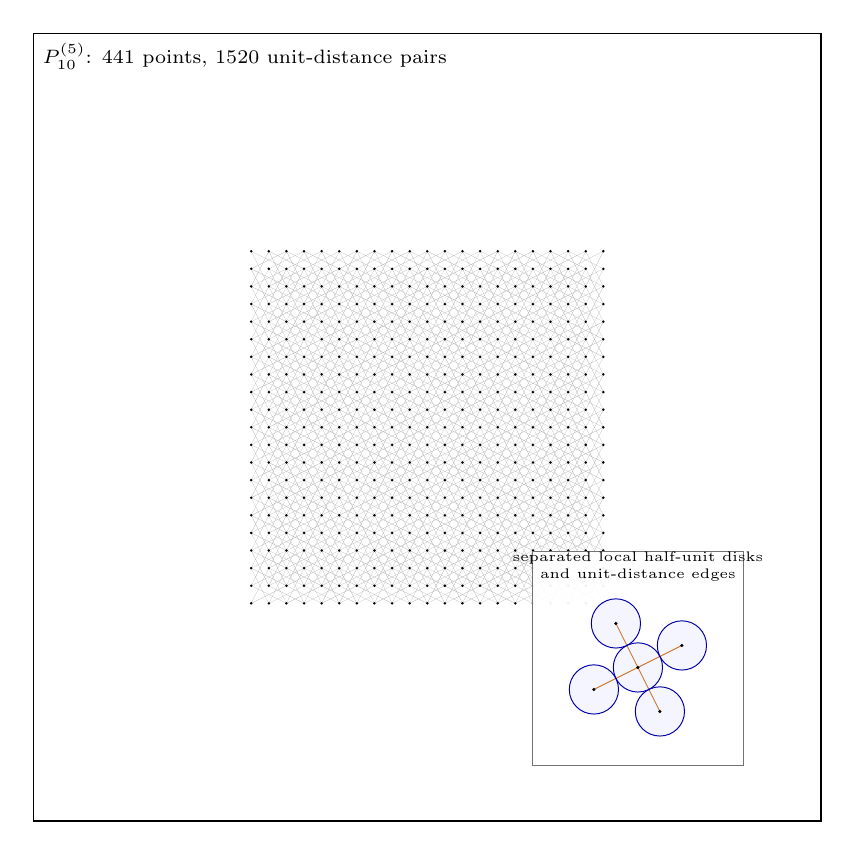
\begin{tikzpicture}[
  scale=0.50,
  edge/.style={draw=black!35, line width=0.055pt},
  pt/.style={circle, fill=black, inner sep=0.11pt},
  boundary/.style={draw=black, line width=0.55pt},
  disk/.style={draw=blue!65!black, fill=blue!18, fill opacity=0.20, line width=0.35pt},
  insetedge/.style={draw=orange!80!black, line width=0.35pt},
  insetpt/.style={circle, fill=black, inner sep=0.45pt}
]
  \clip (-10.15,-10.15) rectangle (10.15,10.15);
  \draw[boundary] (-10,-10) rectangle (10,10);
  \draw[edge] (-4.472,-4.472) -- (-4.025,-3.578);
  \draw[edge] (-4.472,-4.472) -- (-3.578,-4.025);
  \draw[edge] (-4.472,-4.025) -- (-4.025,-3.130);
  \draw[edge] (-4.472,-4.025) -- (-3.578,-3.578);
  \draw[edge] (-4.472,-4.025) -- (-3.578,-4.472);
  \draw[edge] (-4.472,-3.578) -- (-4.025,-2.683);
  \draw[edge] (-4.472,-3.578) -- (-4.025,-4.472);
  \draw[edge] (-4.472,-3.578) -- (-3.578,-3.130);
  \draw[edge] (-4.472,-3.578) -- (-3.578,-4.025);
  \draw[edge] (-4.472,-3.130) -- (-4.025,-2.236);
  \draw[edge] (-4.472,-3.130) -- (-4.025,-4.025);
  \draw[edge] (-4.472,-3.130) -- (-3.578,-2.683);
  \draw[edge] (-4.472,-3.130) -- (-3.578,-3.578);
  \draw[edge] (-4.472,-2.683) -- (-4.025,-1.789);
  \draw[edge] (-4.472,-2.683) -- (-4.025,-3.578);
  \draw[edge] (-4.472,-2.683) -- (-3.578,-2.236);
  \draw[edge] (-4.472,-2.683) -- (-3.578,-3.130);
  \draw[edge] (-4.472,-2.236) -- (-4.025,-1.342);
  \draw[edge] (-4.472,-2.236) -- (-4.025,-3.130);
  \draw[edge] (-4.472,-2.236) -- (-3.578,-1.789);
  \draw[edge] (-4.472,-2.236) -- (-3.578,-2.683);
  \draw[edge] (-4.472,-1.789) -- (-4.025,-0.894);
  \draw[edge] (-4.472,-1.789) -- (-4.025,-2.683);
  \draw[edge] (-4.472,-1.789) -- (-3.578,-1.342);
  \draw[edge] (-4.472,-1.789) -- (-3.578,-2.236);
  \draw[edge] (-4.472,-1.342) -- (-4.025,-0.447);
  \draw[edge] (-4.472,-1.342) -- (-4.025,-2.236);
  \draw[edge] (-4.472,-1.342) -- (-3.578,-0.894);
  \draw[edge] (-4.472,-1.342) -- (-3.578,-1.789);
  \draw[edge] (-4.472,-0.894) -- (-4.025,0.000);
  \draw[edge] (-4.472,-0.894) -- (-4.025,-1.789);
  \draw[edge] (-4.472,-0.894) -- (-3.578,-0.447);
  \draw[edge] (-4.472,-0.894) -- (-3.578,-1.342);
  \draw[edge] (-4.472,-0.447) -- (-4.025,0.447);
  \draw[edge] (-4.472,-0.447) -- (-4.025,-1.342);
  \draw[edge] (-4.472,-0.447) -- (-3.578,0.000);
  \draw[edge] (-4.472,-0.447) -- (-3.578,-0.894);
  \draw[edge] (-4.472,0.000) -- (-4.025,0.894);
  \draw[edge] (-4.472,0.000) -- (-4.025,-0.894);
  \draw[edge] (-4.472,0.000) -- (-3.578,0.447);
  \draw[edge] (-4.472,0.000) -- (-3.578,-0.447);
  \draw[edge] (-4.472,0.447) -- (-4.025,1.342);
  \draw[edge] (-4.472,0.447) -- (-4.025,-0.447);
  \draw[edge] (-4.472,0.447) -- (-3.578,0.894);
  \draw[edge] (-4.472,0.447) -- (-3.578,0.000);
  \draw[edge] (-4.472,0.894) -- (-4.025,1.789);
  \draw[edge] (-4.472,0.894) -- (-4.025,0.000);
  \draw[edge] (-4.472,0.894) -- (-3.578,1.342);
  \draw[edge] (-4.472,0.894) -- (-3.578,0.447);
  \draw[edge] (-4.472,1.342) -- (-4.025,2.236);
  \draw[edge] (-4.472,1.342) -- (-4.025,0.447);
  \draw[edge] (-4.472,1.342) -- (-3.578,1.789);
  \draw[edge] (-4.472,1.342) -- (-3.578,0.894);
  \draw[edge] (-4.472,1.789) -- (-4.025,2.683);
  \draw[edge] (-4.472,1.789) -- (-4.025,0.894);
  \draw[edge] (-4.472,1.789) -- (-3.578,2.236);
  \draw[edge] (-4.472,1.789) -- (-3.578,1.342);
  \draw[edge] (-4.472,2.236) -- (-4.025,3.130);
  \draw[edge] (-4.472,2.236) -- (-4.025,1.342);
  \draw[edge] (-4.472,2.236) -- (-3.578,2.683);
  \draw[edge] (-4.472,2.236) -- (-3.578,1.789);
  \draw[edge] (-4.472,2.683) -- (-4.025,3.578);
  \draw[edge] (-4.472,2.683) -- (-4.025,1.789);
  \draw[edge] (-4.472,2.683) -- (-3.578,3.130);
  \draw[edge] (-4.472,2.683) -- (-3.578,2.236);
  \draw[edge] (-4.472,3.130) -- (-4.025,4.025);
  \draw[edge] (-4.472,3.130) -- (-4.025,2.236);
  \draw[edge] (-4.472,3.130) -- (-3.578,3.578);
  \draw[edge] (-4.472,3.130) -- (-3.578,2.683);
  \draw[edge] (-4.472,3.578) -- (-4.025,4.472);
  \draw[edge] (-4.472,3.578) -- (-4.025,2.683);
  \draw[edge] (-4.472,3.578) -- (-3.578,4.025);
  \draw[edge] (-4.472,3.578) -- (-3.578,3.130);
  \draw[edge] (-4.472,4.025) -- (-4.025,3.130);
  \draw[edge] (-4.472,4.025) -- (-3.578,4.472);
  \draw[edge] (-4.472,4.025) -- (-3.578,3.578);
  \draw[edge] (-4.472,4.472) -- (-4.025,3.578);
  \draw[edge] (-4.472,4.472) -- (-3.578,4.025);
  \draw[edge] (-4.025,-4.472) -- (-3.578,-3.578);
  \draw[edge] (-4.025,-4.472) -- (-3.130,-4.025);
  \draw[edge] (-4.025,-4.025) -- (-3.578,-3.130);
  \draw[edge] (-4.025,-4.025) -- (-3.130,-3.578);
  \draw[edge] (-4.025,-4.025) -- (-3.130,-4.472);
  \draw[edge] (-4.025,-3.578) -- (-3.578,-2.683);
  \draw[edge] (-4.025,-3.578) -- (-3.578,-4.472);
  \draw[edge] (-4.025,-3.578) -- (-3.130,-3.130);
  \draw[edge] (-4.025,-3.578) -- (-3.130,-4.025);
  \draw[edge] (-4.025,-3.130) -- (-3.578,-2.236);
  \draw[edge] (-4.025,-3.130) -- (-3.578,-4.025);
  \draw[edge] (-4.025,-3.130) -- (-3.130,-2.683);
  \draw[edge] (-4.025,-3.130) -- (-3.130,-3.578);
  \draw[edge] (-4.025,-2.683) -- (-3.578,-1.789);
  \draw[edge] (-4.025,-2.683) -- (-3.578,-3.578);
  \draw[edge] (-4.025,-2.683) -- (-3.130,-2.236);
  \draw[edge] (-4.025,-2.683) -- (-3.130,-3.130);
  \draw[edge] (-4.025,-2.236) -- (-3.578,-1.342);
  \draw[edge] (-4.025,-2.236) -- (-3.578,-3.130);
  \draw[edge] (-4.025,-2.236) -- (-3.130,-1.789);
  \draw[edge] (-4.025,-2.236) -- (-3.130,-2.683);
  \draw[edge] (-4.025,-1.789) -- (-3.578,-0.894);
  \draw[edge] (-4.025,-1.789) -- (-3.578,-2.683);
  \draw[edge] (-4.025,-1.789) -- (-3.130,-1.342);
  \draw[edge] (-4.025,-1.789) -- (-3.130,-2.236);
  \draw[edge] (-4.025,-1.342) -- (-3.578,-0.447);
  \draw[edge] (-4.025,-1.342) -- (-3.578,-2.236);
  \draw[edge] (-4.025,-1.342) -- (-3.130,-0.894);
  \draw[edge] (-4.025,-1.342) -- (-3.130,-1.789);
  \draw[edge] (-4.025,-0.894) -- (-3.578,0.000);
  \draw[edge] (-4.025,-0.894) -- (-3.578,-1.789);
  \draw[edge] (-4.025,-0.894) -- (-3.130,-0.447);
  \draw[edge] (-4.025,-0.894) -- (-3.130,-1.342);
  \draw[edge] (-4.025,-0.447) -- (-3.578,0.447);
  \draw[edge] (-4.025,-0.447) -- (-3.578,-1.342);
  \draw[edge] (-4.025,-0.447) -- (-3.130,0.000);
  \draw[edge] (-4.025,-0.447) -- (-3.130,-0.894);
  \draw[edge] (-4.025,0.000) -- (-3.578,0.894);
  \draw[edge] (-4.025,0.000) -- (-3.578,-0.894);
  \draw[edge] (-4.025,0.000) -- (-3.130,0.447);
  \draw[edge] (-4.025,0.000) -- (-3.130,-0.447);
  \draw[edge] (-4.025,0.447) -- (-3.578,1.342);
  \draw[edge] (-4.025,0.447) -- (-3.578,-0.447);
  \draw[edge] (-4.025,0.447) -- (-3.130,0.894);
  \draw[edge] (-4.025,0.447) -- (-3.130,0.000);
  \draw[edge] (-4.025,0.894) -- (-3.578,1.789);
  \draw[edge] (-4.025,0.894) -- (-3.578,0.000);
  \draw[edge] (-4.025,0.894) -- (-3.130,1.342);
  \draw[edge] (-4.025,0.894) -- (-3.130,0.447);
  \draw[edge] (-4.025,1.342) -- (-3.578,2.236);
  \draw[edge] (-4.025,1.342) -- (-3.578,0.447);
  \draw[edge] (-4.025,1.342) -- (-3.130,1.789);
  \draw[edge] (-4.025,1.342) -- (-3.130,0.894);
  \draw[edge] (-4.025,1.789) -- (-3.578,2.683);
  \draw[edge] (-4.025,1.789) -- (-3.578,0.894);
  \draw[edge] (-4.025,1.789) -- (-3.130,2.236);
  \draw[edge] (-4.025,1.789) -- (-3.130,1.342);
  \draw[edge] (-4.025,2.236) -- (-3.578,3.130);
  \draw[edge] (-4.025,2.236) -- (-3.578,1.342);
  \draw[edge] (-4.025,2.236) -- (-3.130,2.683);
  \draw[edge] (-4.025,2.236) -- (-3.130,1.789);
  \draw[edge] (-4.025,2.683) -- (-3.578,3.578);
  \draw[edge] (-4.025,2.683) -- (-3.578,1.789);
  \draw[edge] (-4.025,2.683) -- (-3.130,3.130);
  \draw[edge] (-4.025,2.683) -- (-3.130,2.236);
  \draw[edge] (-4.025,3.130) -- (-3.578,4.025);
  \draw[edge] (-4.025,3.130) -- (-3.578,2.236);
  \draw[edge] (-4.025,3.130) -- (-3.130,3.578);
  \draw[edge] (-4.025,3.130) -- (-3.130,2.683);
  \draw[edge] (-4.025,3.578) -- (-3.578,4.472);
  \draw[edge] (-4.025,3.578) -- (-3.578,2.683);
  \draw[edge] (-4.025,3.578) -- (-3.130,4.025);
  \draw[edge] (-4.025,3.578) -- (-3.130,3.130);
  \draw[edge] (-4.025,4.025) -- (-3.578,3.130);
  \draw[edge] (-4.025,4.025) -- (-3.130,4.472);
  \draw[edge] (-4.025,4.025) -- (-3.130,3.578);
  \draw[edge] (-4.025,4.472) -- (-3.578,3.578);
  \draw[edge] (-4.025,4.472) -- (-3.130,4.025);
  \draw[edge] (-3.578,-4.472) -- (-3.130,-3.578);
  \draw[edge] (-3.578,-4.472) -- (-2.683,-4.025);
  \draw[edge] (-3.578,-4.025) -- (-3.130,-3.130);
  \draw[edge] (-3.578,-4.025) -- (-2.683,-3.578);
  \draw[edge] (-3.578,-4.025) -- (-2.683,-4.472);
  \draw[edge] (-3.578,-3.578) -- (-3.130,-2.683);
  \draw[edge] (-3.578,-3.578) -- (-3.130,-4.472);
  \draw[edge] (-3.578,-3.578) -- (-2.683,-3.130);
  \draw[edge] (-3.578,-3.578) -- (-2.683,-4.025);
  \draw[edge] (-3.578,-3.130) -- (-3.130,-2.236);
  \draw[edge] (-3.578,-3.130) -- (-3.130,-4.025);
  \draw[edge] (-3.578,-3.130) -- (-2.683,-2.683);
  \draw[edge] (-3.578,-3.130) -- (-2.683,-3.578);
  \draw[edge] (-3.578,-2.683) -- (-3.130,-1.789);
  \draw[edge] (-3.578,-2.683) -- (-3.130,-3.578);
  \draw[edge] (-3.578,-2.683) -- (-2.683,-2.236);
  \draw[edge] (-3.578,-2.683) -- (-2.683,-3.130);
  \draw[edge] (-3.578,-2.236) -- (-3.130,-1.342);
  \draw[edge] (-3.578,-2.236) -- (-3.130,-3.130);
  \draw[edge] (-3.578,-2.236) -- (-2.683,-1.789);
  \draw[edge] (-3.578,-2.236) -- (-2.683,-2.683);
  \draw[edge] (-3.578,-1.789) -- (-3.130,-0.894);
  \draw[edge] (-3.578,-1.789) -- (-3.130,-2.683);
  \draw[edge] (-3.578,-1.789) -- (-2.683,-1.342);
  \draw[edge] (-3.578,-1.789) -- (-2.683,-2.236);
  \draw[edge] (-3.578,-1.342) -- (-3.130,-0.447);
  \draw[edge] (-3.578,-1.342) -- (-3.130,-2.236);
  \draw[edge] (-3.578,-1.342) -- (-2.683,-0.894);
  \draw[edge] (-3.578,-1.342) -- (-2.683,-1.789);
  \draw[edge] (-3.578,-0.894) -- (-3.130,0.000);
  \draw[edge] (-3.578,-0.894) -- (-3.130,-1.789);
  \draw[edge] (-3.578,-0.894) -- (-2.683,-0.447);
  \draw[edge] (-3.578,-0.894) -- (-2.683,-1.342);
  \draw[edge] (-3.578,-0.447) -- (-3.130,0.447);
  \draw[edge] (-3.578,-0.447) -- (-3.130,-1.342);
  \draw[edge] (-3.578,-0.447) -- (-2.683,0.000);
  \draw[edge] (-3.578,-0.447) -- (-2.683,-0.894);
  \draw[edge] (-3.578,0.000) -- (-3.130,0.894);
  \draw[edge] (-3.578,0.000) -- (-3.130,-0.894);
  \draw[edge] (-3.578,0.000) -- (-2.683,0.447);
  \draw[edge] (-3.578,0.000) -- (-2.683,-0.447);
  \draw[edge] (-3.578,0.447) -- (-3.130,1.342);
  \draw[edge] (-3.578,0.447) -- (-3.130,-0.447);
  \draw[edge] (-3.578,0.447) -- (-2.683,0.894);
  \draw[edge] (-3.578,0.447) -- (-2.683,0.000);
  \draw[edge] (-3.578,0.894) -- (-3.130,1.789);
  \draw[edge] (-3.578,0.894) -- (-3.130,0.000);
  \draw[edge] (-3.578,0.894) -- (-2.683,1.342);
  \draw[edge] (-3.578,0.894) -- (-2.683,0.447);
  \draw[edge] (-3.578,1.342) -- (-3.130,2.236);
  \draw[edge] (-3.578,1.342) -- (-3.130,0.447);
  \draw[edge] (-3.578,1.342) -- (-2.683,1.789);
  \draw[edge] (-3.578,1.342) -- (-2.683,0.894);
  \draw[edge] (-3.578,1.789) -- (-3.130,2.683);
  \draw[edge] (-3.578,1.789) -- (-3.130,0.894);
  \draw[edge] (-3.578,1.789) -- (-2.683,2.236);
  \draw[edge] (-3.578,1.789) -- (-2.683,1.342);
  \draw[edge] (-3.578,2.236) -- (-3.130,3.130);
  \draw[edge] (-3.578,2.236) -- (-3.130,1.342);
  \draw[edge] (-3.578,2.236) -- (-2.683,2.683);
  \draw[edge] (-3.578,2.236) -- (-2.683,1.789);
  \draw[edge] (-3.578,2.683) -- (-3.130,3.578);
  \draw[edge] (-3.578,2.683) -- (-3.130,1.789);
  \draw[edge] (-3.578,2.683) -- (-2.683,3.130);
  \draw[edge] (-3.578,2.683) -- (-2.683,2.236);
  \draw[edge] (-3.578,3.130) -- (-3.130,4.025);
  \draw[edge] (-3.578,3.130) -- (-3.130,2.236);
  \draw[edge] (-3.578,3.130) -- (-2.683,3.578);
  \draw[edge] (-3.578,3.130) -- (-2.683,2.683);
  \draw[edge] (-3.578,3.578) -- (-3.130,4.472);
  \draw[edge] (-3.578,3.578) -- (-3.130,2.683);
  \draw[edge] (-3.578,3.578) -- (-2.683,4.025);
  \draw[edge] (-3.578,3.578) -- (-2.683,3.130);
  \draw[edge] (-3.578,4.025) -- (-3.130,3.130);
  \draw[edge] (-3.578,4.025) -- (-2.683,4.472);
  \draw[edge] (-3.578,4.025) -- (-2.683,3.578);
  \draw[edge] (-3.578,4.472) -- (-3.130,3.578);
  \draw[edge] (-3.578,4.472) -- (-2.683,4.025);
  \draw[edge] (-3.130,-4.472) -- (-2.683,-3.578);
  \draw[edge] (-3.130,-4.472) -- (-2.236,-4.025);
  \draw[edge] (-3.130,-4.025) -- (-2.683,-3.130);
  \draw[edge] (-3.130,-4.025) -- (-2.236,-3.578);
  \draw[edge] (-3.130,-4.025) -- (-2.236,-4.472);
  \draw[edge] (-3.130,-3.578) -- (-2.683,-2.683);
  \draw[edge] (-3.130,-3.578) -- (-2.683,-4.472);
  \draw[edge] (-3.130,-3.578) -- (-2.236,-3.130);
  \draw[edge] (-3.130,-3.578) -- (-2.236,-4.025);
  \draw[edge] (-3.130,-3.130) -- (-2.683,-2.236);
  \draw[edge] (-3.130,-3.130) -- (-2.683,-4.025);
  \draw[edge] (-3.130,-3.130) -- (-2.236,-2.683);
  \draw[edge] (-3.130,-3.130) -- (-2.236,-3.578);
  \draw[edge] (-3.130,-2.683) -- (-2.683,-1.789);
  \draw[edge] (-3.130,-2.683) -- (-2.683,-3.578);
  \draw[edge] (-3.130,-2.683) -- (-2.236,-2.236);
  \draw[edge] (-3.130,-2.683) -- (-2.236,-3.130);
  \draw[edge] (-3.130,-2.236) -- (-2.683,-1.342);
  \draw[edge] (-3.130,-2.236) -- (-2.683,-3.130);
  \draw[edge] (-3.130,-2.236) -- (-2.236,-1.789);
  \draw[edge] (-3.130,-2.236) -- (-2.236,-2.683);
  \draw[edge] (-3.130,-1.789) -- (-2.683,-0.894);
  \draw[edge] (-3.130,-1.789) -- (-2.683,-2.683);
  \draw[edge] (-3.130,-1.789) -- (-2.236,-1.342);
  \draw[edge] (-3.130,-1.789) -- (-2.236,-2.236);
  \draw[edge] (-3.130,-1.342) -- (-2.683,-0.447);
  \draw[edge] (-3.130,-1.342) -- (-2.683,-2.236);
  \draw[edge] (-3.130,-1.342) -- (-2.236,-0.894);
  \draw[edge] (-3.130,-1.342) -- (-2.236,-1.789);
  \draw[edge] (-3.130,-0.894) -- (-2.683,0.000);
  \draw[edge] (-3.130,-0.894) -- (-2.683,-1.789);
  \draw[edge] (-3.130,-0.894) -- (-2.236,-0.447);
  \draw[edge] (-3.130,-0.894) -- (-2.236,-1.342);
  \draw[edge] (-3.130,-0.447) -- (-2.683,0.447);
  \draw[edge] (-3.130,-0.447) -- (-2.683,-1.342);
  \draw[edge] (-3.130,-0.447) -- (-2.236,0.000);
  \draw[edge] (-3.130,-0.447) -- (-2.236,-0.894);
  \draw[edge] (-3.130,0.000) -- (-2.683,0.894);
  \draw[edge] (-3.130,0.000) -- (-2.683,-0.894);
  \draw[edge] (-3.130,0.000) -- (-2.236,0.447);
  \draw[edge] (-3.130,0.000) -- (-2.236,-0.447);
  \draw[edge] (-3.130,0.447) -- (-2.683,1.342);
  \draw[edge] (-3.130,0.447) -- (-2.683,-0.447);
  \draw[edge] (-3.130,0.447) -- (-2.236,0.894);
  \draw[edge] (-3.130,0.447) -- (-2.236,0.000);
  \draw[edge] (-3.130,0.894) -- (-2.683,1.789);
  \draw[edge] (-3.130,0.894) -- (-2.683,0.000);
  \draw[edge] (-3.130,0.894) -- (-2.236,1.342);
  \draw[edge] (-3.130,0.894) -- (-2.236,0.447);
  \draw[edge] (-3.130,1.342) -- (-2.683,2.236);
  \draw[edge] (-3.130,1.342) -- (-2.683,0.447);
  \draw[edge] (-3.130,1.342) -- (-2.236,1.789);
  \draw[edge] (-3.130,1.342) -- (-2.236,0.894);
  \draw[edge] (-3.130,1.789) -- (-2.683,2.683);
  \draw[edge] (-3.130,1.789) -- (-2.683,0.894);
  \draw[edge] (-3.130,1.789) -- (-2.236,2.236);
  \draw[edge] (-3.130,1.789) -- (-2.236,1.342);
  \draw[edge] (-3.130,2.236) -- (-2.683,3.130);
  \draw[edge] (-3.130,2.236) -- (-2.683,1.342);
  \draw[edge] (-3.130,2.236) -- (-2.236,2.683);
  \draw[edge] (-3.130,2.236) -- (-2.236,1.789);
  \draw[edge] (-3.130,2.683) -- (-2.683,3.578);
  \draw[edge] (-3.130,2.683) -- (-2.683,1.789);
  \draw[edge] (-3.130,2.683) -- (-2.236,3.130);
  \draw[edge] (-3.130,2.683) -- (-2.236,2.236);
  \draw[edge] (-3.130,3.130) -- (-2.683,4.025);
  \draw[edge] (-3.130,3.130) -- (-2.683,2.236);
  \draw[edge] (-3.130,3.130) -- (-2.236,3.578);
  \draw[edge] (-3.130,3.130) -- (-2.236,2.683);
  \draw[edge] (-3.130,3.578) -- (-2.683,4.472);
  \draw[edge] (-3.130,3.578) -- (-2.683,2.683);
  \draw[edge] (-3.130,3.578) -- (-2.236,4.025);
  \draw[edge] (-3.130,3.578) -- (-2.236,3.130);
  \draw[edge] (-3.130,4.025) -- (-2.683,3.130);
  \draw[edge] (-3.130,4.025) -- (-2.236,4.472);
  \draw[edge] (-3.130,4.025) -- (-2.236,3.578);
  \draw[edge] (-3.130,4.472) -- (-2.683,3.578);
  \draw[edge] (-3.130,4.472) -- (-2.236,4.025);
  \draw[edge] (-2.683,-4.472) -- (-2.236,-3.578);
  \draw[edge] (-2.683,-4.472) -- (-1.789,-4.025);
  \draw[edge] (-2.683,-4.025) -- (-2.236,-3.130);
  \draw[edge] (-2.683,-4.025) -- (-1.789,-3.578);
  \draw[edge] (-2.683,-4.025) -- (-1.789,-4.472);
  \draw[edge] (-2.683,-3.578) -- (-2.236,-2.683);
  \draw[edge] (-2.683,-3.578) -- (-2.236,-4.472);
  \draw[edge] (-2.683,-3.578) -- (-1.789,-3.130);
  \draw[edge] (-2.683,-3.578) -- (-1.789,-4.025);
  \draw[edge] (-2.683,-3.130) -- (-2.236,-2.236);
  \draw[edge] (-2.683,-3.130) -- (-2.236,-4.025);
  \draw[edge] (-2.683,-3.130) -- (-1.789,-2.683);
  \draw[edge] (-2.683,-3.130) -- (-1.789,-3.578);
  \draw[edge] (-2.683,-2.683) -- (-2.236,-1.789);
  \draw[edge] (-2.683,-2.683) -- (-2.236,-3.578);
  \draw[edge] (-2.683,-2.683) -- (-1.789,-2.236);
  \draw[edge] (-2.683,-2.683) -- (-1.789,-3.130);
  \draw[edge] (-2.683,-2.236) -- (-2.236,-1.342);
  \draw[edge] (-2.683,-2.236) -- (-2.236,-3.130);
  \draw[edge] (-2.683,-2.236) -- (-1.789,-1.789);
  \draw[edge] (-2.683,-2.236) -- (-1.789,-2.683);
  \draw[edge] (-2.683,-1.789) -- (-2.236,-0.894);
  \draw[edge] (-2.683,-1.789) -- (-2.236,-2.683);
  \draw[edge] (-2.683,-1.789) -- (-1.789,-1.342);
  \draw[edge] (-2.683,-1.789) -- (-1.789,-2.236);
  \draw[edge] (-2.683,-1.342) -- (-2.236,-0.447);
  \draw[edge] (-2.683,-1.342) -- (-2.236,-2.236);
  \draw[edge] (-2.683,-1.342) -- (-1.789,-0.894);
  \draw[edge] (-2.683,-1.342) -- (-1.789,-1.789);
  \draw[edge] (-2.683,-0.894) -- (-2.236,0.000);
  \draw[edge] (-2.683,-0.894) -- (-2.236,-1.789);
  \draw[edge] (-2.683,-0.894) -- (-1.789,-0.447);
  \draw[edge] (-2.683,-0.894) -- (-1.789,-1.342);
  \draw[edge] (-2.683,-0.447) -- (-2.236,0.447);
  \draw[edge] (-2.683,-0.447) -- (-2.236,-1.342);
  \draw[edge] (-2.683,-0.447) -- (-1.789,0.000);
  \draw[edge] (-2.683,-0.447) -- (-1.789,-0.894);
  \draw[edge] (-2.683,0.000) -- (-2.236,0.894);
  \draw[edge] (-2.683,0.000) -- (-2.236,-0.894);
  \draw[edge] (-2.683,0.000) -- (-1.789,0.447);
  \draw[edge] (-2.683,0.000) -- (-1.789,-0.447);
  \draw[edge] (-2.683,0.447) -- (-2.236,1.342);
  \draw[edge] (-2.683,0.447) -- (-2.236,-0.447);
  \draw[edge] (-2.683,0.447) -- (-1.789,0.894);
  \draw[edge] (-2.683,0.447) -- (-1.789,0.000);
  \draw[edge] (-2.683,0.894) -- (-2.236,1.789);
  \draw[edge] (-2.683,0.894) -- (-2.236,0.000);
  \draw[edge] (-2.683,0.894) -- (-1.789,1.342);
  \draw[edge] (-2.683,0.894) -- (-1.789,0.447);
  \draw[edge] (-2.683,1.342) -- (-2.236,2.236);
  \draw[edge] (-2.683,1.342) -- (-2.236,0.447);
  \draw[edge] (-2.683,1.342) -- (-1.789,1.789);
  \draw[edge] (-2.683,1.342) -- (-1.789,0.894);
  \draw[edge] (-2.683,1.789) -- (-2.236,2.683);
  \draw[edge] (-2.683,1.789) -- (-2.236,0.894);
  \draw[edge] (-2.683,1.789) -- (-1.789,2.236);
  \draw[edge] (-2.683,1.789) -- (-1.789,1.342);
  \draw[edge] (-2.683,2.236) -- (-2.236,3.130);
  \draw[edge] (-2.683,2.236) -- (-2.236,1.342);
  \draw[edge] (-2.683,2.236) -- (-1.789,2.683);
  \draw[edge] (-2.683,2.236) -- (-1.789,1.789);
  \draw[edge] (-2.683,2.683) -- (-2.236,3.578);
  \draw[edge] (-2.683,2.683) -- (-2.236,1.789);
  \draw[edge] (-2.683,2.683) -- (-1.789,3.130);
  \draw[edge] (-2.683,2.683) -- (-1.789,2.236);
  \draw[edge] (-2.683,3.130) -- (-2.236,4.025);
  \draw[edge] (-2.683,3.130) -- (-2.236,2.236);
  \draw[edge] (-2.683,3.130) -- (-1.789,3.578);
  \draw[edge] (-2.683,3.130) -- (-1.789,2.683);
  \draw[edge] (-2.683,3.578) -- (-2.236,4.472);
  \draw[edge] (-2.683,3.578) -- (-2.236,2.683);
  \draw[edge] (-2.683,3.578) -- (-1.789,4.025);
  \draw[edge] (-2.683,3.578) -- (-1.789,3.130);
  \draw[edge] (-2.683,4.025) -- (-2.236,3.130);
  \draw[edge] (-2.683,4.025) -- (-1.789,4.472);
  \draw[edge] (-2.683,4.025) -- (-1.789,3.578);
  \draw[edge] (-2.683,4.472) -- (-2.236,3.578);
  \draw[edge] (-2.683,4.472) -- (-1.789,4.025);
  \draw[edge] (-2.236,-4.472) -- (-1.789,-3.578);
  \draw[edge] (-2.236,-4.472) -- (-1.342,-4.025);
  \draw[edge] (-2.236,-4.025) -- (-1.789,-3.130);
  \draw[edge] (-2.236,-4.025) -- (-1.342,-3.578);
  \draw[edge] (-2.236,-4.025) -- (-1.342,-4.472);
  \draw[edge] (-2.236,-3.578) -- (-1.789,-2.683);
  \draw[edge] (-2.236,-3.578) -- (-1.789,-4.472);
  \draw[edge] (-2.236,-3.578) -- (-1.342,-3.130);
  \draw[edge] (-2.236,-3.578) -- (-1.342,-4.025);
  \draw[edge] (-2.236,-3.130) -- (-1.789,-2.236);
  \draw[edge] (-2.236,-3.130) -- (-1.789,-4.025);
  \draw[edge] (-2.236,-3.130) -- (-1.342,-2.683);
  \draw[edge] (-2.236,-3.130) -- (-1.342,-3.578);
  \draw[edge] (-2.236,-2.683) -- (-1.789,-1.789);
  \draw[edge] (-2.236,-2.683) -- (-1.789,-3.578);
  \draw[edge] (-2.236,-2.683) -- (-1.342,-2.236);
  \draw[edge] (-2.236,-2.683) -- (-1.342,-3.130);
  \draw[edge] (-2.236,-2.236) -- (-1.789,-1.342);
  \draw[edge] (-2.236,-2.236) -- (-1.789,-3.130);
  \draw[edge] (-2.236,-2.236) -- (-1.342,-1.789);
  \draw[edge] (-2.236,-2.236) -- (-1.342,-2.683);
  \draw[edge] (-2.236,-1.789) -- (-1.789,-0.894);
  \draw[edge] (-2.236,-1.789) -- (-1.789,-2.683);
  \draw[edge] (-2.236,-1.789) -- (-1.342,-1.342);
  \draw[edge] (-2.236,-1.789) -- (-1.342,-2.236);
  \draw[edge] (-2.236,-1.342) -- (-1.789,-0.447);
  \draw[edge] (-2.236,-1.342) -- (-1.789,-2.236);
  \draw[edge] (-2.236,-1.342) -- (-1.342,-0.894);
  \draw[edge] (-2.236,-1.342) -- (-1.342,-1.789);
  \draw[edge] (-2.236,-0.894) -- (-1.789,0.000);
  \draw[edge] (-2.236,-0.894) -- (-1.789,-1.789);
  \draw[edge] (-2.236,-0.894) -- (-1.342,-0.447);
  \draw[edge] (-2.236,-0.894) -- (-1.342,-1.342);
  \draw[edge] (-2.236,-0.447) -- (-1.789,0.447);
  \draw[edge] (-2.236,-0.447) -- (-1.789,-1.342);
  \draw[edge] (-2.236,-0.447) -- (-1.342,0.000);
  \draw[edge] (-2.236,-0.447) -- (-1.342,-0.894);
  \draw[edge] (-2.236,0.000) -- (-1.789,0.894);
  \draw[edge] (-2.236,0.000) -- (-1.789,-0.894);
  \draw[edge] (-2.236,0.000) -- (-1.342,0.447);
  \draw[edge] (-2.236,0.000) -- (-1.342,-0.447);
  \draw[edge] (-2.236,0.447) -- (-1.789,1.342);
  \draw[edge] (-2.236,0.447) -- (-1.789,-0.447);
  \draw[edge] (-2.236,0.447) -- (-1.342,0.894);
  \draw[edge] (-2.236,0.447) -- (-1.342,0.000);
  \draw[edge] (-2.236,0.894) -- (-1.789,1.789);
  \draw[edge] (-2.236,0.894) -- (-1.789,0.000);
  \draw[edge] (-2.236,0.894) -- (-1.342,1.342);
  \draw[edge] (-2.236,0.894) -- (-1.342,0.447);
  \draw[edge] (-2.236,1.342) -- (-1.789,2.236);
  \draw[edge] (-2.236,1.342) -- (-1.789,0.447);
  \draw[edge] (-2.236,1.342) -- (-1.342,1.789);
  \draw[edge] (-2.236,1.342) -- (-1.342,0.894);
  \draw[edge] (-2.236,1.789) -- (-1.789,2.683);
  \draw[edge] (-2.236,1.789) -- (-1.789,0.894);
  \draw[edge] (-2.236,1.789) -- (-1.342,2.236);
  \draw[edge] (-2.236,1.789) -- (-1.342,1.342);
  \draw[edge] (-2.236,2.236) -- (-1.789,3.130);
  \draw[edge] (-2.236,2.236) -- (-1.789,1.342);
  \draw[edge] (-2.236,2.236) -- (-1.342,2.683);
  \draw[edge] (-2.236,2.236) -- (-1.342,1.789);
  \draw[edge] (-2.236,2.683) -- (-1.789,3.578);
  \draw[edge] (-2.236,2.683) -- (-1.789,1.789);
  \draw[edge] (-2.236,2.683) -- (-1.342,3.130);
  \draw[edge] (-2.236,2.683) -- (-1.342,2.236);
  \draw[edge] (-2.236,3.130) -- (-1.789,4.025);
  \draw[edge] (-2.236,3.130) -- (-1.789,2.236);
  \draw[edge] (-2.236,3.130) -- (-1.342,3.578);
  \draw[edge] (-2.236,3.130) -- (-1.342,2.683);
  \draw[edge] (-2.236,3.578) -- (-1.789,4.472);
  \draw[edge] (-2.236,3.578) -- (-1.789,2.683);
  \draw[edge] (-2.236,3.578) -- (-1.342,4.025);
  \draw[edge] (-2.236,3.578) -- (-1.342,3.130);
  \draw[edge] (-2.236,4.025) -- (-1.789,3.130);
  \draw[edge] (-2.236,4.025) -- (-1.342,4.472);
  \draw[edge] (-2.236,4.025) -- (-1.342,3.578);
  \draw[edge] (-2.236,4.472) -- (-1.789,3.578);
  \draw[edge] (-2.236,4.472) -- (-1.342,4.025);
  \draw[edge] (-1.789,-4.472) -- (-1.342,-3.578);
  \draw[edge] (-1.789,-4.472) -- (-0.894,-4.025);
  \draw[edge] (-1.789,-4.025) -- (-1.342,-3.130);
  \draw[edge] (-1.789,-4.025) -- (-0.894,-3.578);
  \draw[edge] (-1.789,-4.025) -- (-0.894,-4.472);
  \draw[edge] (-1.789,-3.578) -- (-1.342,-2.683);
  \draw[edge] (-1.789,-3.578) -- (-1.342,-4.472);
  \draw[edge] (-1.789,-3.578) -- (-0.894,-3.130);
  \draw[edge] (-1.789,-3.578) -- (-0.894,-4.025);
  \draw[edge] (-1.789,-3.130) -- (-1.342,-2.236);
  \draw[edge] (-1.789,-3.130) -- (-1.342,-4.025);
  \draw[edge] (-1.789,-3.130) -- (-0.894,-2.683);
  \draw[edge] (-1.789,-3.130) -- (-0.894,-3.578);
  \draw[edge] (-1.789,-2.683) -- (-1.342,-1.789);
  \draw[edge] (-1.789,-2.683) -- (-1.342,-3.578);
  \draw[edge] (-1.789,-2.683) -- (-0.894,-2.236);
  \draw[edge] (-1.789,-2.683) -- (-0.894,-3.130);
  \draw[edge] (-1.789,-2.236) -- (-1.342,-1.342);
  \draw[edge] (-1.789,-2.236) -- (-1.342,-3.130);
  \draw[edge] (-1.789,-2.236) -- (-0.894,-1.789);
  \draw[edge] (-1.789,-2.236) -- (-0.894,-2.683);
  \draw[edge] (-1.789,-1.789) -- (-1.342,-0.894);
  \draw[edge] (-1.789,-1.789) -- (-1.342,-2.683);
  \draw[edge] (-1.789,-1.789) -- (-0.894,-1.342);
  \draw[edge] (-1.789,-1.789) -- (-0.894,-2.236);
  \draw[edge] (-1.789,-1.342) -- (-1.342,-0.447);
  \draw[edge] (-1.789,-1.342) -- (-1.342,-2.236);
  \draw[edge] (-1.789,-1.342) -- (-0.894,-0.894);
  \draw[edge] (-1.789,-1.342) -- (-0.894,-1.789);
  \draw[edge] (-1.789,-0.894) -- (-1.342,0.000);
  \draw[edge] (-1.789,-0.894) -- (-1.342,-1.789);
  \draw[edge] (-1.789,-0.894) -- (-0.894,-0.447);
  \draw[edge] (-1.789,-0.894) -- (-0.894,-1.342);
  \draw[edge] (-1.789,-0.447) -- (-1.342,0.447);
  \draw[edge] (-1.789,-0.447) -- (-1.342,-1.342);
  \draw[edge] (-1.789,-0.447) -- (-0.894,0.000);
  \draw[edge] (-1.789,-0.447) -- (-0.894,-0.894);
  \draw[edge] (-1.789,0.000) -- (-1.342,0.894);
  \draw[edge] (-1.789,0.000) -- (-1.342,-0.894);
  \draw[edge] (-1.789,0.000) -- (-0.894,0.447);
  \draw[edge] (-1.789,0.000) -- (-0.894,-0.447);
  \draw[edge] (-1.789,0.447) -- (-1.342,1.342);
  \draw[edge] (-1.789,0.447) -- (-1.342,-0.447);
  \draw[edge] (-1.789,0.447) -- (-0.894,0.894);
  \draw[edge] (-1.789,0.447) -- (-0.894,0.000);
  \draw[edge] (-1.789,0.894) -- (-1.342,1.789);
  \draw[edge] (-1.789,0.894) -- (-1.342,0.000);
  \draw[edge] (-1.789,0.894) -- (-0.894,1.342);
  \draw[edge] (-1.789,0.894) -- (-0.894,0.447);
  \draw[edge] (-1.789,1.342) -- (-1.342,2.236);
  \draw[edge] (-1.789,1.342) -- (-1.342,0.447);
  \draw[edge] (-1.789,1.342) -- (-0.894,1.789);
  \draw[edge] (-1.789,1.342) -- (-0.894,0.894);
  \draw[edge] (-1.789,1.789) -- (-1.342,2.683);
  \draw[edge] (-1.789,1.789) -- (-1.342,0.894);
  \draw[edge] (-1.789,1.789) -- (-0.894,2.236);
  \draw[edge] (-1.789,1.789) -- (-0.894,1.342);
  \draw[edge] (-1.789,2.236) -- (-1.342,3.130);
  \draw[edge] (-1.789,2.236) -- (-1.342,1.342);
  \draw[edge] (-1.789,2.236) -- (-0.894,2.683);
  \draw[edge] (-1.789,2.236) -- (-0.894,1.789);
  \draw[edge] (-1.789,2.683) -- (-1.342,3.578);
  \draw[edge] (-1.789,2.683) -- (-1.342,1.789);
  \draw[edge] (-1.789,2.683) -- (-0.894,3.130);
  \draw[edge] (-1.789,2.683) -- (-0.894,2.236);
  \draw[edge] (-1.789,3.130) -- (-1.342,4.025);
  \draw[edge] (-1.789,3.130) -- (-1.342,2.236);
  \draw[edge] (-1.789,3.130) -- (-0.894,3.578);
  \draw[edge] (-1.789,3.130) -- (-0.894,2.683);
  \draw[edge] (-1.789,3.578) -- (-1.342,4.472);
  \draw[edge] (-1.789,3.578) -- (-1.342,2.683);
  \draw[edge] (-1.789,3.578) -- (-0.894,4.025);
  \draw[edge] (-1.789,3.578) -- (-0.894,3.130);
  \draw[edge] (-1.789,4.025) -- (-1.342,3.130);
  \draw[edge] (-1.789,4.025) -- (-0.894,4.472);
  \draw[edge] (-1.789,4.025) -- (-0.894,3.578);
  \draw[edge] (-1.789,4.472) -- (-1.342,3.578);
  \draw[edge] (-1.789,4.472) -- (-0.894,4.025);
  \draw[edge] (-1.342,-4.472) -- (-0.894,-3.578);
  \draw[edge] (-1.342,-4.472) -- (-0.447,-4.025);
  \draw[edge] (-1.342,-4.025) -- (-0.894,-3.130);
  \draw[edge] (-1.342,-4.025) -- (-0.447,-3.578);
  \draw[edge] (-1.342,-4.025) -- (-0.447,-4.472);
  \draw[edge] (-1.342,-3.578) -- (-0.894,-2.683);
  \draw[edge] (-1.342,-3.578) -- (-0.894,-4.472);
  \draw[edge] (-1.342,-3.578) -- (-0.447,-3.130);
  \draw[edge] (-1.342,-3.578) -- (-0.447,-4.025);
  \draw[edge] (-1.342,-3.130) -- (-0.894,-2.236);
  \draw[edge] (-1.342,-3.130) -- (-0.894,-4.025);
  \draw[edge] (-1.342,-3.130) -- (-0.447,-2.683);
  \draw[edge] (-1.342,-3.130) -- (-0.447,-3.578);
  \draw[edge] (-1.342,-2.683) -- (-0.894,-1.789);
  \draw[edge] (-1.342,-2.683) -- (-0.894,-3.578);
  \draw[edge] (-1.342,-2.683) -- (-0.447,-2.236);
  \draw[edge] (-1.342,-2.683) -- (-0.447,-3.130);
  \draw[edge] (-1.342,-2.236) -- (-0.894,-1.342);
  \draw[edge] (-1.342,-2.236) -- (-0.894,-3.130);
  \draw[edge] (-1.342,-2.236) -- (-0.447,-1.789);
  \draw[edge] (-1.342,-2.236) -- (-0.447,-2.683);
  \draw[edge] (-1.342,-1.789) -- (-0.894,-0.894);
  \draw[edge] (-1.342,-1.789) -- (-0.894,-2.683);
  \draw[edge] (-1.342,-1.789) -- (-0.447,-1.342);
  \draw[edge] (-1.342,-1.789) -- (-0.447,-2.236);
  \draw[edge] (-1.342,-1.342) -- (-0.894,-0.447);
  \draw[edge] (-1.342,-1.342) -- (-0.894,-2.236);
  \draw[edge] (-1.342,-1.342) -- (-0.447,-0.894);
  \draw[edge] (-1.342,-1.342) -- (-0.447,-1.789);
  \draw[edge] (-1.342,-0.894) -- (-0.894,0.000);
  \draw[edge] (-1.342,-0.894) -- (-0.894,-1.789);
  \draw[edge] (-1.342,-0.894) -- (-0.447,-0.447);
  \draw[edge] (-1.342,-0.894) -- (-0.447,-1.342);
  \draw[edge] (-1.342,-0.447) -- (-0.894,0.447);
  \draw[edge] (-1.342,-0.447) -- (-0.894,-1.342);
  \draw[edge] (-1.342,-0.447) -- (-0.447,0.000);
  \draw[edge] (-1.342,-0.447) -- (-0.447,-0.894);
  \draw[edge] (-1.342,0.000) -- (-0.894,0.894);
  \draw[edge] (-1.342,0.000) -- (-0.894,-0.894);
  \draw[edge] (-1.342,0.000) -- (-0.447,0.447);
  \draw[edge] (-1.342,0.000) -- (-0.447,-0.447);
  \draw[edge] (-1.342,0.447) -- (-0.894,1.342);
  \draw[edge] (-1.342,0.447) -- (-0.894,-0.447);
  \draw[edge] (-1.342,0.447) -- (-0.447,0.894);
  \draw[edge] (-1.342,0.447) -- (-0.447,0.000);
  \draw[edge] (-1.342,0.894) -- (-0.894,1.789);
  \draw[edge] (-1.342,0.894) -- (-0.894,0.000);
  \draw[edge] (-1.342,0.894) -- (-0.447,1.342);
  \draw[edge] (-1.342,0.894) -- (-0.447,0.447);
  \draw[edge] (-1.342,1.342) -- (-0.894,2.236);
  \draw[edge] (-1.342,1.342) -- (-0.894,0.447);
  \draw[edge] (-1.342,1.342) -- (-0.447,1.789);
  \draw[edge] (-1.342,1.342) -- (-0.447,0.894);
  \draw[edge] (-1.342,1.789) -- (-0.894,2.683);
  \draw[edge] (-1.342,1.789) -- (-0.894,0.894);
  \draw[edge] (-1.342,1.789) -- (-0.447,2.236);
  \draw[edge] (-1.342,1.789) -- (-0.447,1.342);
  \draw[edge] (-1.342,2.236) -- (-0.894,3.130);
  \draw[edge] (-1.342,2.236) -- (-0.894,1.342);
  \draw[edge] (-1.342,2.236) -- (-0.447,2.683);
  \draw[edge] (-1.342,2.236) -- (-0.447,1.789);
  \draw[edge] (-1.342,2.683) -- (-0.894,3.578);
  \draw[edge] (-1.342,2.683) -- (-0.894,1.789);
  \draw[edge] (-1.342,2.683) -- (-0.447,3.130);
  \draw[edge] (-1.342,2.683) -- (-0.447,2.236);
  \draw[edge] (-1.342,3.130) -- (-0.894,4.025);
  \draw[edge] (-1.342,3.130) -- (-0.894,2.236);
  \draw[edge] (-1.342,3.130) -- (-0.447,3.578);
  \draw[edge] (-1.342,3.130) -- (-0.447,2.683);
  \draw[edge] (-1.342,3.578) -- (-0.894,4.472);
  \draw[edge] (-1.342,3.578) -- (-0.894,2.683);
  \draw[edge] (-1.342,3.578) -- (-0.447,4.025);
  \draw[edge] (-1.342,3.578) -- (-0.447,3.130);
  \draw[edge] (-1.342,4.025) -- (-0.894,3.130);
  \draw[edge] (-1.342,4.025) -- (-0.447,4.472);
  \draw[edge] (-1.342,4.025) -- (-0.447,3.578);
  \draw[edge] (-1.342,4.472) -- (-0.894,3.578);
  \draw[edge] (-1.342,4.472) -- (-0.447,4.025);
  \draw[edge] (-0.894,-4.472) -- (-0.447,-3.578);
  \draw[edge] (-0.894,-4.472) -- (0.000,-4.025);
  \draw[edge] (-0.894,-4.025) -- (-0.447,-3.130);
  \draw[edge] (-0.894,-4.025) -- (0.000,-3.578);
  \draw[edge] (-0.894,-4.025) -- (0.000,-4.472);
  \draw[edge] (-0.894,-3.578) -- (-0.447,-2.683);
  \draw[edge] (-0.894,-3.578) -- (-0.447,-4.472);
  \draw[edge] (-0.894,-3.578) -- (0.000,-3.130);
  \draw[edge] (-0.894,-3.578) -- (0.000,-4.025);
  \draw[edge] (-0.894,-3.130) -- (-0.447,-2.236);
  \draw[edge] (-0.894,-3.130) -- (-0.447,-4.025);
  \draw[edge] (-0.894,-3.130) -- (0.000,-2.683);
  \draw[edge] (-0.894,-3.130) -- (0.000,-3.578);
  \draw[edge] (-0.894,-2.683) -- (-0.447,-1.789);
  \draw[edge] (-0.894,-2.683) -- (-0.447,-3.578);
  \draw[edge] (-0.894,-2.683) -- (0.000,-2.236);
  \draw[edge] (-0.894,-2.683) -- (0.000,-3.130);
  \draw[edge] (-0.894,-2.236) -- (-0.447,-1.342);
  \draw[edge] (-0.894,-2.236) -- (-0.447,-3.130);
  \draw[edge] (-0.894,-2.236) -- (0.000,-1.789);
  \draw[edge] (-0.894,-2.236) -- (0.000,-2.683);
  \draw[edge] (-0.894,-1.789) -- (-0.447,-0.894);
  \draw[edge] (-0.894,-1.789) -- (-0.447,-2.683);
  \draw[edge] (-0.894,-1.789) -- (0.000,-1.342);
  \draw[edge] (-0.894,-1.789) -- (0.000,-2.236);
  \draw[edge] (-0.894,-1.342) -- (-0.447,-0.447);
  \draw[edge] (-0.894,-1.342) -- (-0.447,-2.236);
  \draw[edge] (-0.894,-1.342) -- (0.000,-0.894);
  \draw[edge] (-0.894,-1.342) -- (0.000,-1.789);
  \draw[edge] (-0.894,-0.894) -- (-0.447,0.000);
  \draw[edge] (-0.894,-0.894) -- (-0.447,-1.789);
  \draw[edge] (-0.894,-0.894) -- (0.000,-0.447);
  \draw[edge] (-0.894,-0.894) -- (0.000,-1.342);
  \draw[edge] (-0.894,-0.447) -- (-0.447,0.447);
  \draw[edge] (-0.894,-0.447) -- (-0.447,-1.342);
  \draw[edge] (-0.894,-0.447) -- (0.000,0.000);
  \draw[edge] (-0.894,-0.447) -- (0.000,-0.894);
  \draw[edge] (-0.894,0.000) -- (-0.447,0.894);
  \draw[edge] (-0.894,0.000) -- (-0.447,-0.894);
  \draw[edge] (-0.894,0.000) -- (0.000,0.447);
  \draw[edge] (-0.894,0.000) -- (0.000,-0.447);
  \draw[edge] (-0.894,0.447) -- (-0.447,1.342);
  \draw[edge] (-0.894,0.447) -- (-0.447,-0.447);
  \draw[edge] (-0.894,0.447) -- (0.000,0.894);
  \draw[edge] (-0.894,0.447) -- (0.000,0.000);
  \draw[edge] (-0.894,0.894) -- (-0.447,1.789);
  \draw[edge] (-0.894,0.894) -- (-0.447,0.000);
  \draw[edge] (-0.894,0.894) -- (0.000,1.342);
  \draw[edge] (-0.894,0.894) -- (0.000,0.447);
  \draw[edge] (-0.894,1.342) -- (-0.447,2.236);
  \draw[edge] (-0.894,1.342) -- (-0.447,0.447);
  \draw[edge] (-0.894,1.342) -- (0.000,1.789);
  \draw[edge] (-0.894,1.342) -- (0.000,0.894);
  \draw[edge] (-0.894,1.789) -- (-0.447,2.683);
  \draw[edge] (-0.894,1.789) -- (-0.447,0.894);
  \draw[edge] (-0.894,1.789) -- (0.000,2.236);
  \draw[edge] (-0.894,1.789) -- (0.000,1.342);
  \draw[edge] (-0.894,2.236) -- (-0.447,3.130);
  \draw[edge] (-0.894,2.236) -- (-0.447,1.342);
  \draw[edge] (-0.894,2.236) -- (0.000,2.683);
  \draw[edge] (-0.894,2.236) -- (0.000,1.789);
  \draw[edge] (-0.894,2.683) -- (-0.447,3.578);
  \draw[edge] (-0.894,2.683) -- (-0.447,1.789);
  \draw[edge] (-0.894,2.683) -- (0.000,3.130);
  \draw[edge] (-0.894,2.683) -- (0.000,2.236);
  \draw[edge] (-0.894,3.130) -- (-0.447,4.025);
  \draw[edge] (-0.894,3.130) -- (-0.447,2.236);
  \draw[edge] (-0.894,3.130) -- (0.000,3.578);
  \draw[edge] (-0.894,3.130) -- (0.000,2.683);
  \draw[edge] (-0.894,3.578) -- (-0.447,4.472);
  \draw[edge] (-0.894,3.578) -- (-0.447,2.683);
  \draw[edge] (-0.894,3.578) -- (0.000,4.025);
  \draw[edge] (-0.894,3.578) -- (0.000,3.130);
  \draw[edge] (-0.894,4.025) -- (-0.447,3.130);
  \draw[edge] (-0.894,4.025) -- (0.000,4.472);
  \draw[edge] (-0.894,4.025) -- (0.000,3.578);
  \draw[edge] (-0.894,4.472) -- (-0.447,3.578);
  \draw[edge] (-0.894,4.472) -- (0.000,4.025);
  \draw[edge] (-0.447,-4.472) -- (0.000,-3.578);
  \draw[edge] (-0.447,-4.472) -- (0.447,-4.025);
  \draw[edge] (-0.447,-4.025) -- (0.000,-3.130);
  \draw[edge] (-0.447,-4.025) -- (0.447,-3.578);
  \draw[edge] (-0.447,-4.025) -- (0.447,-4.472);
  \draw[edge] (-0.447,-3.578) -- (0.000,-2.683);
  \draw[edge] (-0.447,-3.578) -- (0.000,-4.472);
  \draw[edge] (-0.447,-3.578) -- (0.447,-3.130);
  \draw[edge] (-0.447,-3.578) -- (0.447,-4.025);
  \draw[edge] (-0.447,-3.130) -- (0.000,-2.236);
  \draw[edge] (-0.447,-3.130) -- (0.000,-4.025);
  \draw[edge] (-0.447,-3.130) -- (0.447,-2.683);
  \draw[edge] (-0.447,-3.130) -- (0.447,-3.578);
  \draw[edge] (-0.447,-2.683) -- (0.000,-1.789);
  \draw[edge] (-0.447,-2.683) -- (0.000,-3.578);
  \draw[edge] (-0.447,-2.683) -- (0.447,-2.236);
  \draw[edge] (-0.447,-2.683) -- (0.447,-3.130);
  \draw[edge] (-0.447,-2.236) -- (0.000,-1.342);
  \draw[edge] (-0.447,-2.236) -- (0.000,-3.130);
  \draw[edge] (-0.447,-2.236) -- (0.447,-1.789);
  \draw[edge] (-0.447,-2.236) -- (0.447,-2.683);
  \draw[edge] (-0.447,-1.789) -- (0.000,-0.894);
  \draw[edge] (-0.447,-1.789) -- (0.000,-2.683);
  \draw[edge] (-0.447,-1.789) -- (0.447,-1.342);
  \draw[edge] (-0.447,-1.789) -- (0.447,-2.236);
  \draw[edge] (-0.447,-1.342) -- (0.000,-0.447);
  \draw[edge] (-0.447,-1.342) -- (0.000,-2.236);
  \draw[edge] (-0.447,-1.342) -- (0.447,-0.894);
  \draw[edge] (-0.447,-1.342) -- (0.447,-1.789);
  \draw[edge] (-0.447,-0.894) -- (0.000,0.000);
  \draw[edge] (-0.447,-0.894) -- (0.000,-1.789);
  \draw[edge] (-0.447,-0.894) -- (0.447,-0.447);
  \draw[edge] (-0.447,-0.894) -- (0.447,-1.342);
  \draw[edge] (-0.447,-0.447) -- (0.000,0.447);
  \draw[edge] (-0.447,-0.447) -- (0.000,-1.342);
  \draw[edge] (-0.447,-0.447) -- (0.447,0.000);
  \draw[edge] (-0.447,-0.447) -- (0.447,-0.894);
  \draw[edge] (-0.447,0.000) -- (0.000,0.894);
  \draw[edge] (-0.447,0.000) -- (0.000,-0.894);
  \draw[edge] (-0.447,0.000) -- (0.447,0.447);
  \draw[edge] (-0.447,0.000) -- (0.447,-0.447);
  \draw[edge] (-0.447,0.447) -- (0.000,1.342);
  \draw[edge] (-0.447,0.447) -- (0.000,-0.447);
  \draw[edge] (-0.447,0.447) -- (0.447,0.894);
  \draw[edge] (-0.447,0.447) -- (0.447,0.000);
  \draw[edge] (-0.447,0.894) -- (0.000,1.789);
  \draw[edge] (-0.447,0.894) -- (0.000,0.000);
  \draw[edge] (-0.447,0.894) -- (0.447,1.342);
  \draw[edge] (-0.447,0.894) -- (0.447,0.447);
  \draw[edge] (-0.447,1.342) -- (0.000,2.236);
  \draw[edge] (-0.447,1.342) -- (0.000,0.447);
  \draw[edge] (-0.447,1.342) -- (0.447,1.789);
  \draw[edge] (-0.447,1.342) -- (0.447,0.894);
  \draw[edge] (-0.447,1.789) -- (0.000,2.683);
  \draw[edge] (-0.447,1.789) -- (0.000,0.894);
  \draw[edge] (-0.447,1.789) -- (0.447,2.236);
  \draw[edge] (-0.447,1.789) -- (0.447,1.342);
  \draw[edge] (-0.447,2.236) -- (0.000,3.130);
  \draw[edge] (-0.447,2.236) -- (0.000,1.342);
  \draw[edge] (-0.447,2.236) -- (0.447,2.683);
  \draw[edge] (-0.447,2.236) -- (0.447,1.789);
  \draw[edge] (-0.447,2.683) -- (0.000,3.578);
  \draw[edge] (-0.447,2.683) -- (0.000,1.789);
  \draw[edge] (-0.447,2.683) -- (0.447,3.130);
  \draw[edge] (-0.447,2.683) -- (0.447,2.236);
  \draw[edge] (-0.447,3.130) -- (0.000,4.025);
  \draw[edge] (-0.447,3.130) -- (0.000,2.236);
  \draw[edge] (-0.447,3.130) -- (0.447,3.578);
  \draw[edge] (-0.447,3.130) -- (0.447,2.683);
  \draw[edge] (-0.447,3.578) -- (0.000,4.472);
  \draw[edge] (-0.447,3.578) -- (0.000,2.683);
  \draw[edge] (-0.447,3.578) -- (0.447,4.025);
  \draw[edge] (-0.447,3.578) -- (0.447,3.130);
  \draw[edge] (-0.447,4.025) -- (0.000,3.130);
  \draw[edge] (-0.447,4.025) -- (0.447,4.472);
  \draw[edge] (-0.447,4.025) -- (0.447,3.578);
  \draw[edge] (-0.447,4.472) -- (0.000,3.578);
  \draw[edge] (-0.447,4.472) -- (0.447,4.025);
  \draw[edge] (0.000,-4.472) -- (0.447,-3.578);
  \draw[edge] (0.000,-4.472) -- (0.894,-4.025);
  \draw[edge] (0.000,-4.025) -- (0.447,-3.130);
  \draw[edge] (0.000,-4.025) -- (0.894,-3.578);
  \draw[edge] (0.000,-4.025) -- (0.894,-4.472);
  \draw[edge] (0.000,-3.578) -- (0.447,-2.683);
  \draw[edge] (0.000,-3.578) -- (0.447,-4.472);
  \draw[edge] (0.000,-3.578) -- (0.894,-3.130);
  \draw[edge] (0.000,-3.578) -- (0.894,-4.025);
  \draw[edge] (0.000,-3.130) -- (0.447,-2.236);
  \draw[edge] (0.000,-3.130) -- (0.447,-4.025);
  \draw[edge] (0.000,-3.130) -- (0.894,-2.683);
  \draw[edge] (0.000,-3.130) -- (0.894,-3.578);
  \draw[edge] (0.000,-2.683) -- (0.447,-1.789);
  \draw[edge] (0.000,-2.683) -- (0.447,-3.578);
  \draw[edge] (0.000,-2.683) -- (0.894,-2.236);
  \draw[edge] (0.000,-2.683) -- (0.894,-3.130);
  \draw[edge] (0.000,-2.236) -- (0.447,-1.342);
  \draw[edge] (0.000,-2.236) -- (0.447,-3.130);
  \draw[edge] (0.000,-2.236) -- (0.894,-1.789);
  \draw[edge] (0.000,-2.236) -- (0.894,-2.683);
  \draw[edge] (0.000,-1.789) -- (0.447,-0.894);
  \draw[edge] (0.000,-1.789) -- (0.447,-2.683);
  \draw[edge] (0.000,-1.789) -- (0.894,-1.342);
  \draw[edge] (0.000,-1.789) -- (0.894,-2.236);
  \draw[edge] (0.000,-1.342) -- (0.447,-0.447);
  \draw[edge] (0.000,-1.342) -- (0.447,-2.236);
  \draw[edge] (0.000,-1.342) -- (0.894,-0.894);
  \draw[edge] (0.000,-1.342) -- (0.894,-1.789);
  \draw[edge] (0.000,-0.894) -- (0.447,0.000);
  \draw[edge] (0.000,-0.894) -- (0.447,-1.789);
  \draw[edge] (0.000,-0.894) -- (0.894,-0.447);
  \draw[edge] (0.000,-0.894) -- (0.894,-1.342);
  \draw[edge] (0.000,-0.447) -- (0.447,0.447);
  \draw[edge] (0.000,-0.447) -- (0.447,-1.342);
  \draw[edge] (0.000,-0.447) -- (0.894,0.000);
  \draw[edge] (0.000,-0.447) -- (0.894,-0.894);
  \draw[edge] (0.000,0.000) -- (0.447,0.894);
  \draw[edge] (0.000,0.000) -- (0.447,-0.894);
  \draw[edge] (0.000,0.000) -- (0.894,0.447);
  \draw[edge] (0.000,0.000) -- (0.894,-0.447);
  \draw[edge] (0.000,0.447) -- (0.447,1.342);
  \draw[edge] (0.000,0.447) -- (0.447,-0.447);
  \draw[edge] (0.000,0.447) -- (0.894,0.894);
  \draw[edge] (0.000,0.447) -- (0.894,0.000);
  \draw[edge] (0.000,0.894) -- (0.447,1.789);
  \draw[edge] (0.000,0.894) -- (0.447,0.000);
  \draw[edge] (0.000,0.894) -- (0.894,1.342);
  \draw[edge] (0.000,0.894) -- (0.894,0.447);
  \draw[edge] (0.000,1.342) -- (0.447,2.236);
  \draw[edge] (0.000,1.342) -- (0.447,0.447);
  \draw[edge] (0.000,1.342) -- (0.894,1.789);
  \draw[edge] (0.000,1.342) -- (0.894,0.894);
  \draw[edge] (0.000,1.789) -- (0.447,2.683);
  \draw[edge] (0.000,1.789) -- (0.447,0.894);
  \draw[edge] (0.000,1.789) -- (0.894,2.236);
  \draw[edge] (0.000,1.789) -- (0.894,1.342);
  \draw[edge] (0.000,2.236) -- (0.447,3.130);
  \draw[edge] (0.000,2.236) -- (0.447,1.342);
  \draw[edge] (0.000,2.236) -- (0.894,2.683);
  \draw[edge] (0.000,2.236) -- (0.894,1.789);
  \draw[edge] (0.000,2.683) -- (0.447,3.578);
  \draw[edge] (0.000,2.683) -- (0.447,1.789);
  \draw[edge] (0.000,2.683) -- (0.894,3.130);
  \draw[edge] (0.000,2.683) -- (0.894,2.236);
  \draw[edge] (0.000,3.130) -- (0.447,4.025);
  \draw[edge] (0.000,3.130) -- (0.447,2.236);
  \draw[edge] (0.000,3.130) -- (0.894,3.578);
  \draw[edge] (0.000,3.130) -- (0.894,2.683);
  \draw[edge] (0.000,3.578) -- (0.447,4.472);
  \draw[edge] (0.000,3.578) -- (0.447,2.683);
  \draw[edge] (0.000,3.578) -- (0.894,4.025);
  \draw[edge] (0.000,3.578) -- (0.894,3.130);
  \draw[edge] (0.000,4.025) -- (0.447,3.130);
  \draw[edge] (0.000,4.025) -- (0.894,4.472);
  \draw[edge] (0.000,4.025) -- (0.894,3.578);
  \draw[edge] (0.000,4.472) -- (0.447,3.578);
  \draw[edge] (0.000,4.472) -- (0.894,4.025);
  \draw[edge] (0.447,-4.472) -- (0.894,-3.578);
  \draw[edge] (0.447,-4.472) -- (1.342,-4.025);
  \draw[edge] (0.447,-4.025) -- (0.894,-3.130);
  \draw[edge] (0.447,-4.025) -- (1.342,-3.578);
  \draw[edge] (0.447,-4.025) -- (1.342,-4.472);
  \draw[edge] (0.447,-3.578) -- (0.894,-2.683);
  \draw[edge] (0.447,-3.578) -- (0.894,-4.472);
  \draw[edge] (0.447,-3.578) -- (1.342,-3.130);
  \draw[edge] (0.447,-3.578) -- (1.342,-4.025);
  \draw[edge] (0.447,-3.130) -- (0.894,-2.236);
  \draw[edge] (0.447,-3.130) -- (0.894,-4.025);
  \draw[edge] (0.447,-3.130) -- (1.342,-2.683);
  \draw[edge] (0.447,-3.130) -- (1.342,-3.578);
  \draw[edge] (0.447,-2.683) -- (0.894,-1.789);
  \draw[edge] (0.447,-2.683) -- (0.894,-3.578);
  \draw[edge] (0.447,-2.683) -- (1.342,-2.236);
  \draw[edge] (0.447,-2.683) -- (1.342,-3.130);
  \draw[edge] (0.447,-2.236) -- (0.894,-1.342);
  \draw[edge] (0.447,-2.236) -- (0.894,-3.130);
  \draw[edge] (0.447,-2.236) -- (1.342,-1.789);
  \draw[edge] (0.447,-2.236) -- (1.342,-2.683);
  \draw[edge] (0.447,-1.789) -- (0.894,-0.894);
  \draw[edge] (0.447,-1.789) -- (0.894,-2.683);
  \draw[edge] (0.447,-1.789) -- (1.342,-1.342);
  \draw[edge] (0.447,-1.789) -- (1.342,-2.236);
  \draw[edge] (0.447,-1.342) -- (0.894,-0.447);
  \draw[edge] (0.447,-1.342) -- (0.894,-2.236);
  \draw[edge] (0.447,-1.342) -- (1.342,-0.894);
  \draw[edge] (0.447,-1.342) -- (1.342,-1.789);
  \draw[edge] (0.447,-0.894) -- (0.894,0.000);
  \draw[edge] (0.447,-0.894) -- (0.894,-1.789);
  \draw[edge] (0.447,-0.894) -- (1.342,-0.447);
  \draw[edge] (0.447,-0.894) -- (1.342,-1.342);
  \draw[edge] (0.447,-0.447) -- (0.894,0.447);
  \draw[edge] (0.447,-0.447) -- (0.894,-1.342);
  \draw[edge] (0.447,-0.447) -- (1.342,0.000);
  \draw[edge] (0.447,-0.447) -- (1.342,-0.894);
  \draw[edge] (0.447,0.000) -- (0.894,0.894);
  \draw[edge] (0.447,0.000) -- (0.894,-0.894);
  \draw[edge] (0.447,0.000) -- (1.342,0.447);
  \draw[edge] (0.447,0.000) -- (1.342,-0.447);
  \draw[edge] (0.447,0.447) -- (0.894,1.342);
  \draw[edge] (0.447,0.447) -- (0.894,-0.447);
  \draw[edge] (0.447,0.447) -- (1.342,0.894);
  \draw[edge] (0.447,0.447) -- (1.342,0.000);
  \draw[edge] (0.447,0.894) -- (0.894,1.789);
  \draw[edge] (0.447,0.894) -- (0.894,0.000);
  \draw[edge] (0.447,0.894) -- (1.342,1.342);
  \draw[edge] (0.447,0.894) -- (1.342,0.447);
  \draw[edge] (0.447,1.342) -- (0.894,2.236);
  \draw[edge] (0.447,1.342) -- (0.894,0.447);
  \draw[edge] (0.447,1.342) -- (1.342,1.789);
  \draw[edge] (0.447,1.342) -- (1.342,0.894);
  \draw[edge] (0.447,1.789) -- (0.894,2.683);
  \draw[edge] (0.447,1.789) -- (0.894,0.894);
  \draw[edge] (0.447,1.789) -- (1.342,2.236);
  \draw[edge] (0.447,1.789) -- (1.342,1.342);
  \draw[edge] (0.447,2.236) -- (0.894,3.130);
  \draw[edge] (0.447,2.236) -- (0.894,1.342);
  \draw[edge] (0.447,2.236) -- (1.342,2.683);
  \draw[edge] (0.447,2.236) -- (1.342,1.789);
  \draw[edge] (0.447,2.683) -- (0.894,3.578);
  \draw[edge] (0.447,2.683) -- (0.894,1.789);
  \draw[edge] (0.447,2.683) -- (1.342,3.130);
  \draw[edge] (0.447,2.683) -- (1.342,2.236);
  \draw[edge] (0.447,3.130) -- (0.894,4.025);
  \draw[edge] (0.447,3.130) -- (0.894,2.236);
  \draw[edge] (0.447,3.130) -- (1.342,3.578);
  \draw[edge] (0.447,3.130) -- (1.342,2.683);
  \draw[edge] (0.447,3.578) -- (0.894,4.472);
  \draw[edge] (0.447,3.578) -- (0.894,2.683);
  \draw[edge] (0.447,3.578) -- (1.342,4.025);
  \draw[edge] (0.447,3.578) -- (1.342,3.130);
  \draw[edge] (0.447,4.025) -- (0.894,3.130);
  \draw[edge] (0.447,4.025) -- (1.342,4.472);
  \draw[edge] (0.447,4.025) -- (1.342,3.578);
  \draw[edge] (0.447,4.472) -- (0.894,3.578);
  \draw[edge] (0.447,4.472) -- (1.342,4.025);
  \draw[edge] (0.894,-4.472) -- (1.342,-3.578);
  \draw[edge] (0.894,-4.472) -- (1.789,-4.025);
  \draw[edge] (0.894,-4.025) -- (1.342,-3.130);
  \draw[edge] (0.894,-4.025) -- (1.789,-3.578);
  \draw[edge] (0.894,-4.025) -- (1.789,-4.472);
  \draw[edge] (0.894,-3.578) -- (1.342,-2.683);
  \draw[edge] (0.894,-3.578) -- (1.342,-4.472);
  \draw[edge] (0.894,-3.578) -- (1.789,-3.130);
  \draw[edge] (0.894,-3.578) -- (1.789,-4.025);
  \draw[edge] (0.894,-3.130) -- (1.342,-2.236);
  \draw[edge] (0.894,-3.130) -- (1.342,-4.025);
  \draw[edge] (0.894,-3.130) -- (1.789,-2.683);
  \draw[edge] (0.894,-3.130) -- (1.789,-3.578);
  \draw[edge] (0.894,-2.683) -- (1.342,-1.789);
  \draw[edge] (0.894,-2.683) -- (1.342,-3.578);
  \draw[edge] (0.894,-2.683) -- (1.789,-2.236);
  \draw[edge] (0.894,-2.683) -- (1.789,-3.130);
  \draw[edge] (0.894,-2.236) -- (1.342,-1.342);
  \draw[edge] (0.894,-2.236) -- (1.342,-3.130);
  \draw[edge] (0.894,-2.236) -- (1.789,-1.789);
  \draw[edge] (0.894,-2.236) -- (1.789,-2.683);
  \draw[edge] (0.894,-1.789) -- (1.342,-0.894);
  \draw[edge] (0.894,-1.789) -- (1.342,-2.683);
  \draw[edge] (0.894,-1.789) -- (1.789,-1.342);
  \draw[edge] (0.894,-1.789) -- (1.789,-2.236);
  \draw[edge] (0.894,-1.342) -- (1.342,-0.447);
  \draw[edge] (0.894,-1.342) -- (1.342,-2.236);
  \draw[edge] (0.894,-1.342) -- (1.789,-0.894);
  \draw[edge] (0.894,-1.342) -- (1.789,-1.789);
  \draw[edge] (0.894,-0.894) -- (1.342,0.000);
  \draw[edge] (0.894,-0.894) -- (1.342,-1.789);
  \draw[edge] (0.894,-0.894) -- (1.789,-0.447);
  \draw[edge] (0.894,-0.894) -- (1.789,-1.342);
  \draw[edge] (0.894,-0.447) -- (1.342,0.447);
  \draw[edge] (0.894,-0.447) -- (1.342,-1.342);
  \draw[edge] (0.894,-0.447) -- (1.789,0.000);
  \draw[edge] (0.894,-0.447) -- (1.789,-0.894);
  \draw[edge] (0.894,0.000) -- (1.342,0.894);
  \draw[edge] (0.894,0.000) -- (1.342,-0.894);
  \draw[edge] (0.894,0.000) -- (1.789,0.447);
  \draw[edge] (0.894,0.000) -- (1.789,-0.447);
  \draw[edge] (0.894,0.447) -- (1.342,1.342);
  \draw[edge] (0.894,0.447) -- (1.342,-0.447);
  \draw[edge] (0.894,0.447) -- (1.789,0.894);
  \draw[edge] (0.894,0.447) -- (1.789,0.000);
  \draw[edge] (0.894,0.894) -- (1.342,1.789);
  \draw[edge] (0.894,0.894) -- (1.342,0.000);
  \draw[edge] (0.894,0.894) -- (1.789,1.342);
  \draw[edge] (0.894,0.894) -- (1.789,0.447);
  \draw[edge] (0.894,1.342) -- (1.342,2.236);
  \draw[edge] (0.894,1.342) -- (1.342,0.447);
  \draw[edge] (0.894,1.342) -- (1.789,1.789);
  \draw[edge] (0.894,1.342) -- (1.789,0.894);
  \draw[edge] (0.894,1.789) -- (1.342,2.683);
  \draw[edge] (0.894,1.789) -- (1.342,0.894);
  \draw[edge] (0.894,1.789) -- (1.789,2.236);
  \draw[edge] (0.894,1.789) -- (1.789,1.342);
  \draw[edge] (0.894,2.236) -- (1.342,3.130);
  \draw[edge] (0.894,2.236) -- (1.342,1.342);
  \draw[edge] (0.894,2.236) -- (1.789,2.683);
  \draw[edge] (0.894,2.236) -- (1.789,1.789);
  \draw[edge] (0.894,2.683) -- (1.342,3.578);
  \draw[edge] (0.894,2.683) -- (1.342,1.789);
  \draw[edge] (0.894,2.683) -- (1.789,3.130);
  \draw[edge] (0.894,2.683) -- (1.789,2.236);
  \draw[edge] (0.894,3.130) -- (1.342,4.025);
  \draw[edge] (0.894,3.130) -- (1.342,2.236);
  \draw[edge] (0.894,3.130) -- (1.789,3.578);
  \draw[edge] (0.894,3.130) -- (1.789,2.683);
  \draw[edge] (0.894,3.578) -- (1.342,4.472);
  \draw[edge] (0.894,3.578) -- (1.342,2.683);
  \draw[edge] (0.894,3.578) -- (1.789,4.025);
  \draw[edge] (0.894,3.578) -- (1.789,3.130);
  \draw[edge] (0.894,4.025) -- (1.342,3.130);
  \draw[edge] (0.894,4.025) -- (1.789,4.472);
  \draw[edge] (0.894,4.025) -- (1.789,3.578);
  \draw[edge] (0.894,4.472) -- (1.342,3.578);
  \draw[edge] (0.894,4.472) -- (1.789,4.025);
  \draw[edge] (1.342,-4.472) -- (1.789,-3.578);
  \draw[edge] (1.342,-4.472) -- (2.236,-4.025);
  \draw[edge] (1.342,-4.025) -- (1.789,-3.130);
  \draw[edge] (1.342,-4.025) -- (2.236,-3.578);
  \draw[edge] (1.342,-4.025) -- (2.236,-4.472);
  \draw[edge] (1.342,-3.578) -- (1.789,-2.683);
  \draw[edge] (1.342,-3.578) -- (1.789,-4.472);
  \draw[edge] (1.342,-3.578) -- (2.236,-3.130);
  \draw[edge] (1.342,-3.578) -- (2.236,-4.025);
  \draw[edge] (1.342,-3.130) -- (1.789,-2.236);
  \draw[edge] (1.342,-3.130) -- (1.789,-4.025);
  \draw[edge] (1.342,-3.130) -- (2.236,-2.683);
  \draw[edge] (1.342,-3.130) -- (2.236,-3.578);
  \draw[edge] (1.342,-2.683) -- (1.789,-1.789);
  \draw[edge] (1.342,-2.683) -- (1.789,-3.578);
  \draw[edge] (1.342,-2.683) -- (2.236,-2.236);
  \draw[edge] (1.342,-2.683) -- (2.236,-3.130);
  \draw[edge] (1.342,-2.236) -- (1.789,-1.342);
  \draw[edge] (1.342,-2.236) -- (1.789,-3.130);
  \draw[edge] (1.342,-2.236) -- (2.236,-1.789);
  \draw[edge] (1.342,-2.236) -- (2.236,-2.683);
  \draw[edge] (1.342,-1.789) -- (1.789,-0.894);
  \draw[edge] (1.342,-1.789) -- (1.789,-2.683);
  \draw[edge] (1.342,-1.789) -- (2.236,-1.342);
  \draw[edge] (1.342,-1.789) -- (2.236,-2.236);
  \draw[edge] (1.342,-1.342) -- (1.789,-0.447);
  \draw[edge] (1.342,-1.342) -- (1.789,-2.236);
  \draw[edge] (1.342,-1.342) -- (2.236,-0.894);
  \draw[edge] (1.342,-1.342) -- (2.236,-1.789);
  \draw[edge] (1.342,-0.894) -- (1.789,0.000);
  \draw[edge] (1.342,-0.894) -- (1.789,-1.789);
  \draw[edge] (1.342,-0.894) -- (2.236,-0.447);
  \draw[edge] (1.342,-0.894) -- (2.236,-1.342);
  \draw[edge] (1.342,-0.447) -- (1.789,0.447);
  \draw[edge] (1.342,-0.447) -- (1.789,-1.342);
  \draw[edge] (1.342,-0.447) -- (2.236,0.000);
  \draw[edge] (1.342,-0.447) -- (2.236,-0.894);
  \draw[edge] (1.342,0.000) -- (1.789,0.894);
  \draw[edge] (1.342,0.000) -- (1.789,-0.894);
  \draw[edge] (1.342,0.000) -- (2.236,0.447);
  \draw[edge] (1.342,0.000) -- (2.236,-0.447);
  \draw[edge] (1.342,0.447) -- (1.789,1.342);
  \draw[edge] (1.342,0.447) -- (1.789,-0.447);
  \draw[edge] (1.342,0.447) -- (2.236,0.894);
  \draw[edge] (1.342,0.447) -- (2.236,0.000);
  \draw[edge] (1.342,0.894) -- (1.789,1.789);
  \draw[edge] (1.342,0.894) -- (1.789,0.000);
  \draw[edge] (1.342,0.894) -- (2.236,1.342);
  \draw[edge] (1.342,0.894) -- (2.236,0.447);
  \draw[edge] (1.342,1.342) -- (1.789,2.236);
  \draw[edge] (1.342,1.342) -- (1.789,0.447);
  \draw[edge] (1.342,1.342) -- (2.236,1.789);
  \draw[edge] (1.342,1.342) -- (2.236,0.894);
  \draw[edge] (1.342,1.789) -- (1.789,2.683);
  \draw[edge] (1.342,1.789) -- (1.789,0.894);
  \draw[edge] (1.342,1.789) -- (2.236,2.236);
  \draw[edge] (1.342,1.789) -- (2.236,1.342);
  \draw[edge] (1.342,2.236) -- (1.789,3.130);
  \draw[edge] (1.342,2.236) -- (1.789,1.342);
  \draw[edge] (1.342,2.236) -- (2.236,2.683);
  \draw[edge] (1.342,2.236) -- (2.236,1.789);
  \draw[edge] (1.342,2.683) -- (1.789,3.578);
  \draw[edge] (1.342,2.683) -- (1.789,1.789);
  \draw[edge] (1.342,2.683) -- (2.236,3.130);
  \draw[edge] (1.342,2.683) -- (2.236,2.236);
  \draw[edge] (1.342,3.130) -- (1.789,4.025);
  \draw[edge] (1.342,3.130) -- (1.789,2.236);
  \draw[edge] (1.342,3.130) -- (2.236,3.578);
  \draw[edge] (1.342,3.130) -- (2.236,2.683);
  \draw[edge] (1.342,3.578) -- (1.789,4.472);
  \draw[edge] (1.342,3.578) -- (1.789,2.683);
  \draw[edge] (1.342,3.578) -- (2.236,4.025);
  \draw[edge] (1.342,3.578) -- (2.236,3.130);
  \draw[edge] (1.342,4.025) -- (1.789,3.130);
  \draw[edge] (1.342,4.025) -- (2.236,4.472);
  \draw[edge] (1.342,4.025) -- (2.236,3.578);
  \draw[edge] (1.342,4.472) -- (1.789,3.578);
  \draw[edge] (1.342,4.472) -- (2.236,4.025);
  \draw[edge] (1.789,-4.472) -- (2.236,-3.578);
  \draw[edge] (1.789,-4.472) -- (2.683,-4.025);
  \draw[edge] (1.789,-4.025) -- (2.236,-3.130);
  \draw[edge] (1.789,-4.025) -- (2.683,-3.578);
  \draw[edge] (1.789,-4.025) -- (2.683,-4.472);
  \draw[edge] (1.789,-3.578) -- (2.236,-2.683);
  \draw[edge] (1.789,-3.578) -- (2.236,-4.472);
  \draw[edge] (1.789,-3.578) -- (2.683,-3.130);
  \draw[edge] (1.789,-3.578) -- (2.683,-4.025);
  \draw[edge] (1.789,-3.130) -- (2.236,-2.236);
  \draw[edge] (1.789,-3.130) -- (2.236,-4.025);
  \draw[edge] (1.789,-3.130) -- (2.683,-2.683);
  \draw[edge] (1.789,-3.130) -- (2.683,-3.578);
  \draw[edge] (1.789,-2.683) -- (2.236,-1.789);
  \draw[edge] (1.789,-2.683) -- (2.236,-3.578);
  \draw[edge] (1.789,-2.683) -- (2.683,-2.236);
  \draw[edge] (1.789,-2.683) -- (2.683,-3.130);
  \draw[edge] (1.789,-2.236) -- (2.236,-1.342);
  \draw[edge] (1.789,-2.236) -- (2.236,-3.130);
  \draw[edge] (1.789,-2.236) -- (2.683,-1.789);
  \draw[edge] (1.789,-2.236) -- (2.683,-2.683);
  \draw[edge] (1.789,-1.789) -- (2.236,-0.894);
  \draw[edge] (1.789,-1.789) -- (2.236,-2.683);
  \draw[edge] (1.789,-1.789) -- (2.683,-1.342);
  \draw[edge] (1.789,-1.789) -- (2.683,-2.236);
  \draw[edge] (1.789,-1.342) -- (2.236,-0.447);
  \draw[edge] (1.789,-1.342) -- (2.236,-2.236);
  \draw[edge] (1.789,-1.342) -- (2.683,-0.894);
  \draw[edge] (1.789,-1.342) -- (2.683,-1.789);
  \draw[edge] (1.789,-0.894) -- (2.236,0.000);
  \draw[edge] (1.789,-0.894) -- (2.236,-1.789);
  \draw[edge] (1.789,-0.894) -- (2.683,-0.447);
  \draw[edge] (1.789,-0.894) -- (2.683,-1.342);
  \draw[edge] (1.789,-0.447) -- (2.236,0.447);
  \draw[edge] (1.789,-0.447) -- (2.236,-1.342);
  \draw[edge] (1.789,-0.447) -- (2.683,0.000);
  \draw[edge] (1.789,-0.447) -- (2.683,-0.894);
  \draw[edge] (1.789,0.000) -- (2.236,0.894);
  \draw[edge] (1.789,0.000) -- (2.236,-0.894);
  \draw[edge] (1.789,0.000) -- (2.683,0.447);
  \draw[edge] (1.789,0.000) -- (2.683,-0.447);
  \draw[edge] (1.789,0.447) -- (2.236,1.342);
  \draw[edge] (1.789,0.447) -- (2.236,-0.447);
  \draw[edge] (1.789,0.447) -- (2.683,0.894);
  \draw[edge] (1.789,0.447) -- (2.683,0.000);
  \draw[edge] (1.789,0.894) -- (2.236,1.789);
  \draw[edge] (1.789,0.894) -- (2.236,0.000);
  \draw[edge] (1.789,0.894) -- (2.683,1.342);
  \draw[edge] (1.789,0.894) -- (2.683,0.447);
  \draw[edge] (1.789,1.342) -- (2.236,2.236);
  \draw[edge] (1.789,1.342) -- (2.236,0.447);
  \draw[edge] (1.789,1.342) -- (2.683,1.789);
  \draw[edge] (1.789,1.342) -- (2.683,0.894);
  \draw[edge] (1.789,1.789) -- (2.236,2.683);
  \draw[edge] (1.789,1.789) -- (2.236,0.894);
  \draw[edge] (1.789,1.789) -- (2.683,2.236);
  \draw[edge] (1.789,1.789) -- (2.683,1.342);
  \draw[edge] (1.789,2.236) -- (2.236,3.130);
  \draw[edge] (1.789,2.236) -- (2.236,1.342);
  \draw[edge] (1.789,2.236) -- (2.683,2.683);
  \draw[edge] (1.789,2.236) -- (2.683,1.789);
  \draw[edge] (1.789,2.683) -- (2.236,3.578);
  \draw[edge] (1.789,2.683) -- (2.236,1.789);
  \draw[edge] (1.789,2.683) -- (2.683,3.130);
  \draw[edge] (1.789,2.683) -- (2.683,2.236);
  \draw[edge] (1.789,3.130) -- (2.236,4.025);
  \draw[edge] (1.789,3.130) -- (2.236,2.236);
  \draw[edge] (1.789,3.130) -- (2.683,3.578);
  \draw[edge] (1.789,3.130) -- (2.683,2.683);
  \draw[edge] (1.789,3.578) -- (2.236,4.472);
  \draw[edge] (1.789,3.578) -- (2.236,2.683);
  \draw[edge] (1.789,3.578) -- (2.683,4.025);
  \draw[edge] (1.789,3.578) -- (2.683,3.130);
  \draw[edge] (1.789,4.025) -- (2.236,3.130);
  \draw[edge] (1.789,4.025) -- (2.683,4.472);
  \draw[edge] (1.789,4.025) -- (2.683,3.578);
  \draw[edge] (1.789,4.472) -- (2.236,3.578);
  \draw[edge] (1.789,4.472) -- (2.683,4.025);
  \draw[edge] (2.236,-4.472) -- (2.683,-3.578);
  \draw[edge] (2.236,-4.472) -- (3.130,-4.025);
  \draw[edge] (2.236,-4.025) -- (2.683,-3.130);
  \draw[edge] (2.236,-4.025) -- (3.130,-3.578);
  \draw[edge] (2.236,-4.025) -- (3.130,-4.472);
  \draw[edge] (2.236,-3.578) -- (2.683,-2.683);
  \draw[edge] (2.236,-3.578) -- (2.683,-4.472);
  \draw[edge] (2.236,-3.578) -- (3.130,-3.130);
  \draw[edge] (2.236,-3.578) -- (3.130,-4.025);
  \draw[edge] (2.236,-3.130) -- (2.683,-2.236);
  \draw[edge] (2.236,-3.130) -- (2.683,-4.025);
  \draw[edge] (2.236,-3.130) -- (3.130,-2.683);
  \draw[edge] (2.236,-3.130) -- (3.130,-3.578);
  \draw[edge] (2.236,-2.683) -- (2.683,-1.789);
  \draw[edge] (2.236,-2.683) -- (2.683,-3.578);
  \draw[edge] (2.236,-2.683) -- (3.130,-2.236);
  \draw[edge] (2.236,-2.683) -- (3.130,-3.130);
  \draw[edge] (2.236,-2.236) -- (2.683,-1.342);
  \draw[edge] (2.236,-2.236) -- (2.683,-3.130);
  \draw[edge] (2.236,-2.236) -- (3.130,-1.789);
  \draw[edge] (2.236,-2.236) -- (3.130,-2.683);
  \draw[edge] (2.236,-1.789) -- (2.683,-0.894);
  \draw[edge] (2.236,-1.789) -- (2.683,-2.683);
  \draw[edge] (2.236,-1.789) -- (3.130,-1.342);
  \draw[edge] (2.236,-1.789) -- (3.130,-2.236);
  \draw[edge] (2.236,-1.342) -- (2.683,-0.447);
  \draw[edge] (2.236,-1.342) -- (2.683,-2.236);
  \draw[edge] (2.236,-1.342) -- (3.130,-0.894);
  \draw[edge] (2.236,-1.342) -- (3.130,-1.789);
  \draw[edge] (2.236,-0.894) -- (2.683,0.000);
  \draw[edge] (2.236,-0.894) -- (2.683,-1.789);
  \draw[edge] (2.236,-0.894) -- (3.130,-0.447);
  \draw[edge] (2.236,-0.894) -- (3.130,-1.342);
  \draw[edge] (2.236,-0.447) -- (2.683,0.447);
  \draw[edge] (2.236,-0.447) -- (2.683,-1.342);
  \draw[edge] (2.236,-0.447) -- (3.130,0.000);
  \draw[edge] (2.236,-0.447) -- (3.130,-0.894);
  \draw[edge] (2.236,0.000) -- (2.683,0.894);
  \draw[edge] (2.236,0.000) -- (2.683,-0.894);
  \draw[edge] (2.236,0.000) -- (3.130,0.447);
  \draw[edge] (2.236,0.000) -- (3.130,-0.447);
  \draw[edge] (2.236,0.447) -- (2.683,1.342);
  \draw[edge] (2.236,0.447) -- (2.683,-0.447);
  \draw[edge] (2.236,0.447) -- (3.130,0.894);
  \draw[edge] (2.236,0.447) -- (3.130,0.000);
  \draw[edge] (2.236,0.894) -- (2.683,1.789);
  \draw[edge] (2.236,0.894) -- (2.683,0.000);
  \draw[edge] (2.236,0.894) -- (3.130,1.342);
  \draw[edge] (2.236,0.894) -- (3.130,0.447);
  \draw[edge] (2.236,1.342) -- (2.683,2.236);
  \draw[edge] (2.236,1.342) -- (2.683,0.447);
  \draw[edge] (2.236,1.342) -- (3.130,1.789);
  \draw[edge] (2.236,1.342) -- (3.130,0.894);
  \draw[edge] (2.236,1.789) -- (2.683,2.683);
  \draw[edge] (2.236,1.789) -- (2.683,0.894);
  \draw[edge] (2.236,1.789) -- (3.130,2.236);
  \draw[edge] (2.236,1.789) -- (3.130,1.342);
  \draw[edge] (2.236,2.236) -- (2.683,3.130);
  \draw[edge] (2.236,2.236) -- (2.683,1.342);
  \draw[edge] (2.236,2.236) -- (3.130,2.683);
  \draw[edge] (2.236,2.236) -- (3.130,1.789);
  \draw[edge] (2.236,2.683) -- (2.683,3.578);
  \draw[edge] (2.236,2.683) -- (2.683,1.789);
  \draw[edge] (2.236,2.683) -- (3.130,3.130);
  \draw[edge] (2.236,2.683) -- (3.130,2.236);
  \draw[edge] (2.236,3.130) -- (2.683,4.025);
  \draw[edge] (2.236,3.130) -- (2.683,2.236);
  \draw[edge] (2.236,3.130) -- (3.130,3.578);
  \draw[edge] (2.236,3.130) -- (3.130,2.683);
  \draw[edge] (2.236,3.578) -- (2.683,4.472);
  \draw[edge] (2.236,3.578) -- (2.683,2.683);
  \draw[edge] (2.236,3.578) -- (3.130,4.025);
  \draw[edge] (2.236,3.578) -- (3.130,3.130);
  \draw[edge] (2.236,4.025) -- (2.683,3.130);
  \draw[edge] (2.236,4.025) -- (3.130,4.472);
  \draw[edge] (2.236,4.025) -- (3.130,3.578);
  \draw[edge] (2.236,4.472) -- (2.683,3.578);
  \draw[edge] (2.236,4.472) -- (3.130,4.025);
  \draw[edge] (2.683,-4.472) -- (3.130,-3.578);
  \draw[edge] (2.683,-4.472) -- (3.578,-4.025);
  \draw[edge] (2.683,-4.025) -- (3.130,-3.130);
  \draw[edge] (2.683,-4.025) -- (3.578,-3.578);
  \draw[edge] (2.683,-4.025) -- (3.578,-4.472);
  \draw[edge] (2.683,-3.578) -- (3.130,-2.683);
  \draw[edge] (2.683,-3.578) -- (3.130,-4.472);
  \draw[edge] (2.683,-3.578) -- (3.578,-3.130);
  \draw[edge] (2.683,-3.578) -- (3.578,-4.025);
  \draw[edge] (2.683,-3.130) -- (3.130,-2.236);
  \draw[edge] (2.683,-3.130) -- (3.130,-4.025);
  \draw[edge] (2.683,-3.130) -- (3.578,-2.683);
  \draw[edge] (2.683,-3.130) -- (3.578,-3.578);
  \draw[edge] (2.683,-2.683) -- (3.130,-1.789);
  \draw[edge] (2.683,-2.683) -- (3.130,-3.578);
  \draw[edge] (2.683,-2.683) -- (3.578,-2.236);
  \draw[edge] (2.683,-2.683) -- (3.578,-3.130);
  \draw[edge] (2.683,-2.236) -- (3.130,-1.342);
  \draw[edge] (2.683,-2.236) -- (3.130,-3.130);
  \draw[edge] (2.683,-2.236) -- (3.578,-1.789);
  \draw[edge] (2.683,-2.236) -- (3.578,-2.683);
  \draw[edge] (2.683,-1.789) -- (3.130,-0.894);
  \draw[edge] (2.683,-1.789) -- (3.130,-2.683);
  \draw[edge] (2.683,-1.789) -- (3.578,-1.342);
  \draw[edge] (2.683,-1.789) -- (3.578,-2.236);
  \draw[edge] (2.683,-1.342) -- (3.130,-0.447);
  \draw[edge] (2.683,-1.342) -- (3.130,-2.236);
  \draw[edge] (2.683,-1.342) -- (3.578,-0.894);
  \draw[edge] (2.683,-1.342) -- (3.578,-1.789);
  \draw[edge] (2.683,-0.894) -- (3.130,0.000);
  \draw[edge] (2.683,-0.894) -- (3.130,-1.789);
  \draw[edge] (2.683,-0.894) -- (3.578,-0.447);
  \draw[edge] (2.683,-0.894) -- (3.578,-1.342);
  \draw[edge] (2.683,-0.447) -- (3.130,0.447);
  \draw[edge] (2.683,-0.447) -- (3.130,-1.342);
  \draw[edge] (2.683,-0.447) -- (3.578,0.000);
  \draw[edge] (2.683,-0.447) -- (3.578,-0.894);
  \draw[edge] (2.683,0.000) -- (3.130,0.894);
  \draw[edge] (2.683,0.000) -- (3.130,-0.894);
  \draw[edge] (2.683,0.000) -- (3.578,0.447);
  \draw[edge] (2.683,0.000) -- (3.578,-0.447);
  \draw[edge] (2.683,0.447) -- (3.130,1.342);
  \draw[edge] (2.683,0.447) -- (3.130,-0.447);
  \draw[edge] (2.683,0.447) -- (3.578,0.894);
  \draw[edge] (2.683,0.447) -- (3.578,0.000);
  \draw[edge] (2.683,0.894) -- (3.130,1.789);
  \draw[edge] (2.683,0.894) -- (3.130,0.000);
  \draw[edge] (2.683,0.894) -- (3.578,1.342);
  \draw[edge] (2.683,0.894) -- (3.578,0.447);
  \draw[edge] (2.683,1.342) -- (3.130,2.236);
  \draw[edge] (2.683,1.342) -- (3.130,0.447);
  \draw[edge] (2.683,1.342) -- (3.578,1.789);
  \draw[edge] (2.683,1.342) -- (3.578,0.894);
  \draw[edge] (2.683,1.789) -- (3.130,2.683);
  \draw[edge] (2.683,1.789) -- (3.130,0.894);
  \draw[edge] (2.683,1.789) -- (3.578,2.236);
  \draw[edge] (2.683,1.789) -- (3.578,1.342);
  \draw[edge] (2.683,2.236) -- (3.130,3.130);
  \draw[edge] (2.683,2.236) -- (3.130,1.342);
  \draw[edge] (2.683,2.236) -- (3.578,2.683);
  \draw[edge] (2.683,2.236) -- (3.578,1.789);
  \draw[edge] (2.683,2.683) -- (3.130,3.578);
  \draw[edge] (2.683,2.683) -- (3.130,1.789);
  \draw[edge] (2.683,2.683) -- (3.578,3.130);
  \draw[edge] (2.683,2.683) -- (3.578,2.236);
  \draw[edge] (2.683,3.130) -- (3.130,4.025);
  \draw[edge] (2.683,3.130) -- (3.130,2.236);
  \draw[edge] (2.683,3.130) -- (3.578,3.578);
  \draw[edge] (2.683,3.130) -- (3.578,2.683);
  \draw[edge] (2.683,3.578) -- (3.130,4.472);
  \draw[edge] (2.683,3.578) -- (3.130,2.683);
  \draw[edge] (2.683,3.578) -- (3.578,4.025);
  \draw[edge] (2.683,3.578) -- (3.578,3.130);
  \draw[edge] (2.683,4.025) -- (3.130,3.130);
  \draw[edge] (2.683,4.025) -- (3.578,4.472);
  \draw[edge] (2.683,4.025) -- (3.578,3.578);
  \draw[edge] (2.683,4.472) -- (3.130,3.578);
  \draw[edge] (2.683,4.472) -- (3.578,4.025);
  \draw[edge] (3.130,-4.472) -- (3.578,-3.578);
  \draw[edge] (3.130,-4.472) -- (4.025,-4.025);
  \draw[edge] (3.130,-4.025) -- (3.578,-3.130);
  \draw[edge] (3.130,-4.025) -- (4.025,-3.578);
  \draw[edge] (3.130,-4.025) -- (4.025,-4.472);
  \draw[edge] (3.130,-3.578) -- (3.578,-2.683);
  \draw[edge] (3.130,-3.578) -- (3.578,-4.472);
  \draw[edge] (3.130,-3.578) -- (4.025,-3.130);
  \draw[edge] (3.130,-3.578) -- (4.025,-4.025);
  \draw[edge] (3.130,-3.130) -- (3.578,-2.236);
  \draw[edge] (3.130,-3.130) -- (3.578,-4.025);
  \draw[edge] (3.130,-3.130) -- (4.025,-2.683);
  \draw[edge] (3.130,-3.130) -- (4.025,-3.578);
  \draw[edge] (3.130,-2.683) -- (3.578,-1.789);
  \draw[edge] (3.130,-2.683) -- (3.578,-3.578);
  \draw[edge] (3.130,-2.683) -- (4.025,-2.236);
  \draw[edge] (3.130,-2.683) -- (4.025,-3.130);
  \draw[edge] (3.130,-2.236) -- (3.578,-1.342);
  \draw[edge] (3.130,-2.236) -- (3.578,-3.130);
  \draw[edge] (3.130,-2.236) -- (4.025,-1.789);
  \draw[edge] (3.130,-2.236) -- (4.025,-2.683);
  \draw[edge] (3.130,-1.789) -- (3.578,-0.894);
  \draw[edge] (3.130,-1.789) -- (3.578,-2.683);
  \draw[edge] (3.130,-1.789) -- (4.025,-1.342);
  \draw[edge] (3.130,-1.789) -- (4.025,-2.236);
  \draw[edge] (3.130,-1.342) -- (3.578,-0.447);
  \draw[edge] (3.130,-1.342) -- (3.578,-2.236);
  \draw[edge] (3.130,-1.342) -- (4.025,-0.894);
  \draw[edge] (3.130,-1.342) -- (4.025,-1.789);
  \draw[edge] (3.130,-0.894) -- (3.578,0.000);
  \draw[edge] (3.130,-0.894) -- (3.578,-1.789);
  \draw[edge] (3.130,-0.894) -- (4.025,-0.447);
  \draw[edge] (3.130,-0.894) -- (4.025,-1.342);
  \draw[edge] (3.130,-0.447) -- (3.578,0.447);
  \draw[edge] (3.130,-0.447) -- (3.578,-1.342);
  \draw[edge] (3.130,-0.447) -- (4.025,0.000);
  \draw[edge] (3.130,-0.447) -- (4.025,-0.894);
  \draw[edge] (3.130,0.000) -- (3.578,0.894);
  \draw[edge] (3.130,0.000) -- (3.578,-0.894);
  \draw[edge] (3.130,0.000) -- (4.025,0.447);
  \draw[edge] (3.130,0.000) -- (4.025,-0.447);
  \draw[edge] (3.130,0.447) -- (3.578,1.342);
  \draw[edge] (3.130,0.447) -- (3.578,-0.447);
  \draw[edge] (3.130,0.447) -- (4.025,0.894);
  \draw[edge] (3.130,0.447) -- (4.025,0.000);
  \draw[edge] (3.130,0.894) -- (3.578,1.789);
  \draw[edge] (3.130,0.894) -- (3.578,0.000);
  \draw[edge] (3.130,0.894) -- (4.025,1.342);
  \draw[edge] (3.130,0.894) -- (4.025,0.447);
  \draw[edge] (3.130,1.342) -- (3.578,2.236);
  \draw[edge] (3.130,1.342) -- (3.578,0.447);
  \draw[edge] (3.130,1.342) -- (4.025,1.789);
  \draw[edge] (3.130,1.342) -- (4.025,0.894);
  \draw[edge] (3.130,1.789) -- (3.578,2.683);
  \draw[edge] (3.130,1.789) -- (3.578,0.894);
  \draw[edge] (3.130,1.789) -- (4.025,2.236);
  \draw[edge] (3.130,1.789) -- (4.025,1.342);
  \draw[edge] (3.130,2.236) -- (3.578,3.130);
  \draw[edge] (3.130,2.236) -- (3.578,1.342);
  \draw[edge] (3.130,2.236) -- (4.025,2.683);
  \draw[edge] (3.130,2.236) -- (4.025,1.789);
  \draw[edge] (3.130,2.683) -- (3.578,3.578);
  \draw[edge] (3.130,2.683) -- (3.578,1.789);
  \draw[edge] (3.130,2.683) -- (4.025,3.130);
  \draw[edge] (3.130,2.683) -- (4.025,2.236);
  \draw[edge] (3.130,3.130) -- (3.578,4.025);
  \draw[edge] (3.130,3.130) -- (3.578,2.236);
  \draw[edge] (3.130,3.130) -- (4.025,3.578);
  \draw[edge] (3.130,3.130) -- (4.025,2.683);
  \draw[edge] (3.130,3.578) -- (3.578,4.472);
  \draw[edge] (3.130,3.578) -- (3.578,2.683);
  \draw[edge] (3.130,3.578) -- (4.025,4.025);
  \draw[edge] (3.130,3.578) -- (4.025,3.130);
  \draw[edge] (3.130,4.025) -- (3.578,3.130);
  \draw[edge] (3.130,4.025) -- (4.025,4.472);
  \draw[edge] (3.130,4.025) -- (4.025,3.578);
  \draw[edge] (3.130,4.472) -- (3.578,3.578);
  \draw[edge] (3.130,4.472) -- (4.025,4.025);
  \draw[edge] (3.578,-4.472) -- (4.025,-3.578);
  \draw[edge] (3.578,-4.472) -- (4.472,-4.025);
  \draw[edge] (3.578,-4.025) -- (4.025,-3.130);
  \draw[edge] (3.578,-4.025) -- (4.472,-3.578);
  \draw[edge] (3.578,-4.025) -- (4.472,-4.472);
  \draw[edge] (3.578,-3.578) -- (4.025,-2.683);
  \draw[edge] (3.578,-3.578) -- (4.025,-4.472);
  \draw[edge] (3.578,-3.578) -- (4.472,-3.130);
  \draw[edge] (3.578,-3.578) -- (4.472,-4.025);
  \draw[edge] (3.578,-3.130) -- (4.025,-2.236);
  \draw[edge] (3.578,-3.130) -- (4.025,-4.025);
  \draw[edge] (3.578,-3.130) -- (4.472,-2.683);
  \draw[edge] (3.578,-3.130) -- (4.472,-3.578);
  \draw[edge] (3.578,-2.683) -- (4.025,-1.789);
  \draw[edge] (3.578,-2.683) -- (4.025,-3.578);
  \draw[edge] (3.578,-2.683) -- (4.472,-2.236);
  \draw[edge] (3.578,-2.683) -- (4.472,-3.130);
  \draw[edge] (3.578,-2.236) -- (4.025,-1.342);
  \draw[edge] (3.578,-2.236) -- (4.025,-3.130);
  \draw[edge] (3.578,-2.236) -- (4.472,-1.789);
  \draw[edge] (3.578,-2.236) -- (4.472,-2.683);
  \draw[edge] (3.578,-1.789) -- (4.025,-0.894);
  \draw[edge] (3.578,-1.789) -- (4.025,-2.683);
  \draw[edge] (3.578,-1.789) -- (4.472,-1.342);
  \draw[edge] (3.578,-1.789) -- (4.472,-2.236);
  \draw[edge] (3.578,-1.342) -- (4.025,-0.447);
  \draw[edge] (3.578,-1.342) -- (4.025,-2.236);
  \draw[edge] (3.578,-1.342) -- (4.472,-0.894);
  \draw[edge] (3.578,-1.342) -- (4.472,-1.789);
  \draw[edge] (3.578,-0.894) -- (4.025,0.000);
  \draw[edge] (3.578,-0.894) -- (4.025,-1.789);
  \draw[edge] (3.578,-0.894) -- (4.472,-0.447);
  \draw[edge] (3.578,-0.894) -- (4.472,-1.342);
  \draw[edge] (3.578,-0.447) -- (4.025,0.447);
  \draw[edge] (3.578,-0.447) -- (4.025,-1.342);
  \draw[edge] (3.578,-0.447) -- (4.472,0.000);
  \draw[edge] (3.578,-0.447) -- (4.472,-0.894);
  \draw[edge] (3.578,0.000) -- (4.025,0.894);
  \draw[edge] (3.578,0.000) -- (4.025,-0.894);
  \draw[edge] (3.578,0.000) -- (4.472,0.447);
  \draw[edge] (3.578,0.000) -- (4.472,-0.447);
  \draw[edge] (3.578,0.447) -- (4.025,1.342);
  \draw[edge] (3.578,0.447) -- (4.025,-0.447);
  \draw[edge] (3.578,0.447) -- (4.472,0.894);
  \draw[edge] (3.578,0.447) -- (4.472,0.000);
  \draw[edge] (3.578,0.894) -- (4.025,1.789);
  \draw[edge] (3.578,0.894) -- (4.025,0.000);
  \draw[edge] (3.578,0.894) -- (4.472,1.342);
  \draw[edge] (3.578,0.894) -- (4.472,0.447);
  \draw[edge] (3.578,1.342) -- (4.025,2.236);
  \draw[edge] (3.578,1.342) -- (4.025,0.447);
  \draw[edge] (3.578,1.342) -- (4.472,1.789);
  \draw[edge] (3.578,1.342) -- (4.472,0.894);
  \draw[edge] (3.578,1.789) -- (4.025,2.683);
  \draw[edge] (3.578,1.789) -- (4.025,0.894);
  \draw[edge] (3.578,1.789) -- (4.472,2.236);
  \draw[edge] (3.578,1.789) -- (4.472,1.342);
  \draw[edge] (3.578,2.236) -- (4.025,3.130);
  \draw[edge] (3.578,2.236) -- (4.025,1.342);
  \draw[edge] (3.578,2.236) -- (4.472,2.683);
  \draw[edge] (3.578,2.236) -- (4.472,1.789);
  \draw[edge] (3.578,2.683) -- (4.025,3.578);
  \draw[edge] (3.578,2.683) -- (4.025,1.789);
  \draw[edge] (3.578,2.683) -- (4.472,3.130);
  \draw[edge] (3.578,2.683) -- (4.472,2.236);
  \draw[edge] (3.578,3.130) -- (4.025,4.025);
  \draw[edge] (3.578,3.130) -- (4.025,2.236);
  \draw[edge] (3.578,3.130) -- (4.472,3.578);
  \draw[edge] (3.578,3.130) -- (4.472,2.683);
  \draw[edge] (3.578,3.578) -- (4.025,4.472);
  \draw[edge] (3.578,3.578) -- (4.025,2.683);
  \draw[edge] (3.578,3.578) -- (4.472,4.025);
  \draw[edge] (3.578,3.578) -- (4.472,3.130);
  \draw[edge] (3.578,4.025) -- (4.025,3.130);
  \draw[edge] (3.578,4.025) -- (4.472,4.472);
  \draw[edge] (3.578,4.025) -- (4.472,3.578);
  \draw[edge] (3.578,4.472) -- (4.025,3.578);
  \draw[edge] (3.578,4.472) -- (4.472,4.025);
  \draw[edge] (4.025,-4.472) -- (4.472,-3.578);
  \draw[edge] (4.025,-4.025) -- (4.472,-3.130);
  \draw[edge] (4.025,-3.578) -- (4.472,-2.683);
  \draw[edge] (4.025,-3.578) -- (4.472,-4.472);
  \draw[edge] (4.025,-3.130) -- (4.472,-2.236);
  \draw[edge] (4.025,-3.130) -- (4.472,-4.025);
  \draw[edge] (4.025,-2.683) -- (4.472,-1.789);
  \draw[edge] (4.025,-2.683) -- (4.472,-3.578);
  \draw[edge] (4.025,-2.236) -- (4.472,-1.342);
  \draw[edge] (4.025,-2.236) -- (4.472,-3.130);
  \draw[edge] (4.025,-1.789) -- (4.472,-0.894);
  \draw[edge] (4.025,-1.789) -- (4.472,-2.683);
  \draw[edge] (4.025,-1.342) -- (4.472,-0.447);
  \draw[edge] (4.025,-1.342) -- (4.472,-2.236);
  \draw[edge] (4.025,-0.894) -- (4.472,0.000);
  \draw[edge] (4.025,-0.894) -- (4.472,-1.789);
  \draw[edge] (4.025,-0.447) -- (4.472,0.447);
  \draw[edge] (4.025,-0.447) -- (4.472,-1.342);
  \draw[edge] (4.025,0.000) -- (4.472,0.894);
  \draw[edge] (4.025,0.000) -- (4.472,-0.894);
  \draw[edge] (4.025,0.447) -- (4.472,1.342);
  \draw[edge] (4.025,0.447) -- (4.472,-0.447);
  \draw[edge] (4.025,0.894) -- (4.472,1.789);
  \draw[edge] (4.025,0.894) -- (4.472,0.000);
  \draw[edge] (4.025,1.342) -- (4.472,2.236);
  \draw[edge] (4.025,1.342) -- (4.472,0.447);
  \draw[edge] (4.025,1.789) -- (4.472,2.683);
  \draw[edge] (4.025,1.789) -- (4.472,0.894);
  \draw[edge] (4.025,2.236) -- (4.472,3.130);
  \draw[edge] (4.025,2.236) -- (4.472,1.342);
  \draw[edge] (4.025,2.683) -- (4.472,3.578);
  \draw[edge] (4.025,2.683) -- (4.472,1.789);
  \draw[edge] (4.025,3.130) -- (4.472,4.025);
  \draw[edge] (4.025,3.130) -- (4.472,2.236);
  \draw[edge] (4.025,3.578) -- (4.472,4.472);
  \draw[edge] (4.025,3.578) -- (4.472,2.683);
  \draw[edge] (4.025,4.025) -- (4.472,3.130);
  \draw[edge] (4.025,4.472) -- (4.472,3.578);
  \node[pt] at (-4.472,-4.472) {};
  \node[pt] at (-4.472,-4.025) {};
  \node[pt] at (-4.472,-3.578) {};
  \node[pt] at (-4.472,-3.130) {};
  \node[pt] at (-4.472,-2.683) {};
  \node[pt] at (-4.472,-2.236) {};
  \node[pt] at (-4.472,-1.789) {};
  \node[pt] at (-4.472,-1.342) {};
  \node[pt] at (-4.472,-0.894) {};
  \node[pt] at (-4.472,-0.447) {};
  \node[pt] at (-4.472,0.000) {};
  \node[pt] at (-4.472,0.447) {};
  \node[pt] at (-4.472,0.894) {};
  \node[pt] at (-4.472,1.342) {};
  \node[pt] at (-4.472,1.789) {};
  \node[pt] at (-4.472,2.236) {};
  \node[pt] at (-4.472,2.683) {};
  \node[pt] at (-4.472,3.130) {};
  \node[pt] at (-4.472,3.578) {};
  \node[pt] at (-4.472,4.025) {};
  \node[pt] at (-4.472,4.472) {};
  \node[pt] at (-4.025,-4.472) {};
  \node[pt] at (-4.025,-4.025) {};
  \node[pt] at (-4.025,-3.578) {};
  \node[pt] at (-4.025,-3.130) {};
  \node[pt] at (-4.025,-2.683) {};
  \node[pt] at (-4.025,-2.236) {};
  \node[pt] at (-4.025,-1.789) {};
  \node[pt] at (-4.025,-1.342) {};
  \node[pt] at (-4.025,-0.894) {};
  \node[pt] at (-4.025,-0.447) {};
  \node[pt] at (-4.025,0.000) {};
  \node[pt] at (-4.025,0.447) {};
  \node[pt] at (-4.025,0.894) {};
  \node[pt] at (-4.025,1.342) {};
  \node[pt] at (-4.025,1.789) {};
  \node[pt] at (-4.025,2.236) {};
  \node[pt] at (-4.025,2.683) {};
  \node[pt] at (-4.025,3.130) {};
  \node[pt] at (-4.025,3.578) {};
  \node[pt] at (-4.025,4.025) {};
  \node[pt] at (-4.025,4.472) {};
  \node[pt] at (-3.578,-4.472) {};
  \node[pt] at (-3.578,-4.025) {};
  \node[pt] at (-3.578,-3.578) {};
  \node[pt] at (-3.578,-3.130) {};
  \node[pt] at (-3.578,-2.683) {};
  \node[pt] at (-3.578,-2.236) {};
  \node[pt] at (-3.578,-1.789) {};
  \node[pt] at (-3.578,-1.342) {};
  \node[pt] at (-3.578,-0.894) {};
  \node[pt] at (-3.578,-0.447) {};
  \node[pt] at (-3.578,0.000) {};
  \node[pt] at (-3.578,0.447) {};
  \node[pt] at (-3.578,0.894) {};
  \node[pt] at (-3.578,1.342) {};
  \node[pt] at (-3.578,1.789) {};
  \node[pt] at (-3.578,2.236) {};
  \node[pt] at (-3.578,2.683) {};
  \node[pt] at (-3.578,3.130) {};
  \node[pt] at (-3.578,3.578) {};
  \node[pt] at (-3.578,4.025) {};
  \node[pt] at (-3.578,4.472) {};
  \node[pt] at (-3.130,-4.472) {};
  \node[pt] at (-3.130,-4.025) {};
  \node[pt] at (-3.130,-3.578) {};
  \node[pt] at (-3.130,-3.130) {};
  \node[pt] at (-3.130,-2.683) {};
  \node[pt] at (-3.130,-2.236) {};
  \node[pt] at (-3.130,-1.789) {};
  \node[pt] at (-3.130,-1.342) {};
  \node[pt] at (-3.130,-0.894) {};
  \node[pt] at (-3.130,-0.447) {};
  \node[pt] at (-3.130,0.000) {};
  \node[pt] at (-3.130,0.447) {};
  \node[pt] at (-3.130,0.894) {};
  \node[pt] at (-3.130,1.342) {};
  \node[pt] at (-3.130,1.789) {};
  \node[pt] at (-3.130,2.236) {};
  \node[pt] at (-3.130,2.683) {};
  \node[pt] at (-3.130,3.130) {};
  \node[pt] at (-3.130,3.578) {};
  \node[pt] at (-3.130,4.025) {};
  \node[pt] at (-3.130,4.472) {};
  \node[pt] at (-2.683,-4.472) {};
  \node[pt] at (-2.683,-4.025) {};
  \node[pt] at (-2.683,-3.578) {};
  \node[pt] at (-2.683,-3.130) {};
  \node[pt] at (-2.683,-2.683) {};
  \node[pt] at (-2.683,-2.236) {};
  \node[pt] at (-2.683,-1.789) {};
  \node[pt] at (-2.683,-1.342) {};
  \node[pt] at (-2.683,-0.894) {};
  \node[pt] at (-2.683,-0.447) {};
  \node[pt] at (-2.683,0.000) {};
  \node[pt] at (-2.683,0.447) {};
  \node[pt] at (-2.683,0.894) {};
  \node[pt] at (-2.683,1.342) {};
  \node[pt] at (-2.683,1.789) {};
  \node[pt] at (-2.683,2.236) {};
  \node[pt] at (-2.683,2.683) {};
  \node[pt] at (-2.683,3.130) {};
  \node[pt] at (-2.683,3.578) {};
  \node[pt] at (-2.683,4.025) {};
  \node[pt] at (-2.683,4.472) {};
  \node[pt] at (-2.236,-4.472) {};
  \node[pt] at (-2.236,-4.025) {};
  \node[pt] at (-2.236,-3.578) {};
  \node[pt] at (-2.236,-3.130) {};
  \node[pt] at (-2.236,-2.683) {};
  \node[pt] at (-2.236,-2.236) {};
  \node[pt] at (-2.236,-1.789) {};
  \node[pt] at (-2.236,-1.342) {};
  \node[pt] at (-2.236,-0.894) {};
  \node[pt] at (-2.236,-0.447) {};
  \node[pt] at (-2.236,0.000) {};
  \node[pt] at (-2.236,0.447) {};
  \node[pt] at (-2.236,0.894) {};
  \node[pt] at (-2.236,1.342) {};
  \node[pt] at (-2.236,1.789) {};
  \node[pt] at (-2.236,2.236) {};
  \node[pt] at (-2.236,2.683) {};
  \node[pt] at (-2.236,3.130) {};
  \node[pt] at (-2.236,3.578) {};
  \node[pt] at (-2.236,4.025) {};
  \node[pt] at (-2.236,4.472) {};
  \node[pt] at (-1.789,-4.472) {};
  \node[pt] at (-1.789,-4.025) {};
  \node[pt] at (-1.789,-3.578) {};
  \node[pt] at (-1.789,-3.130) {};
  \node[pt] at (-1.789,-2.683) {};
  \node[pt] at (-1.789,-2.236) {};
  \node[pt] at (-1.789,-1.789) {};
  \node[pt] at (-1.789,-1.342) {};
  \node[pt] at (-1.789,-0.894) {};
  \node[pt] at (-1.789,-0.447) {};
  \node[pt] at (-1.789,0.000) {};
  \node[pt] at (-1.789,0.447) {};
  \node[pt] at (-1.789,0.894) {};
  \node[pt] at (-1.789,1.342) {};
  \node[pt] at (-1.789,1.789) {};
  \node[pt] at (-1.789,2.236) {};
  \node[pt] at (-1.789,2.683) {};
  \node[pt] at (-1.789,3.130) {};
  \node[pt] at (-1.789,3.578) {};
  \node[pt] at (-1.789,4.025) {};
  \node[pt] at (-1.789,4.472) {};
  \node[pt] at (-1.342,-4.472) {};
  \node[pt] at (-1.342,-4.025) {};
  \node[pt] at (-1.342,-3.578) {};
  \node[pt] at (-1.342,-3.130) {};
  \node[pt] at (-1.342,-2.683) {};
  \node[pt] at (-1.342,-2.236) {};
  \node[pt] at (-1.342,-1.789) {};
  \node[pt] at (-1.342,-1.342) {};
  \node[pt] at (-1.342,-0.894) {};
  \node[pt] at (-1.342,-0.447) {};
  \node[pt] at (-1.342,0.000) {};
  \node[pt] at (-1.342,0.447) {};
  \node[pt] at (-1.342,0.894) {};
  \node[pt] at (-1.342,1.342) {};
  \node[pt] at (-1.342,1.789) {};
  \node[pt] at (-1.342,2.236) {};
  \node[pt] at (-1.342,2.683) {};
  \node[pt] at (-1.342,3.130) {};
  \node[pt] at (-1.342,3.578) {};
  \node[pt] at (-1.342,4.025) {};
  \node[pt] at (-1.342,4.472) {};
  \node[pt] at (-0.894,-4.472) {};
  \node[pt] at (-0.894,-4.025) {};
  \node[pt] at (-0.894,-3.578) {};
  \node[pt] at (-0.894,-3.130) {};
  \node[pt] at (-0.894,-2.683) {};
  \node[pt] at (-0.894,-2.236) {};
  \node[pt] at (-0.894,-1.789) {};
  \node[pt] at (-0.894,-1.342) {};
  \node[pt] at (-0.894,-0.894) {};
  \node[pt] at (-0.894,-0.447) {};
  \node[pt] at (-0.894,0.000) {};
  \node[pt] at (-0.894,0.447) {};
  \node[pt] at (-0.894,0.894) {};
  \node[pt] at (-0.894,1.342) {};
  \node[pt] at (-0.894,1.789) {};
  \node[pt] at (-0.894,2.236) {};
  \node[pt] at (-0.894,2.683) {};
  \node[pt] at (-0.894,3.130) {};
  \node[pt] at (-0.894,3.578) {};
  \node[pt] at (-0.894,4.025) {};
  \node[pt] at (-0.894,4.472) {};
  \node[pt] at (-0.447,-4.472) {};
  \node[pt] at (-0.447,-4.025) {};
  \node[pt] at (-0.447,-3.578) {};
  \node[pt] at (-0.447,-3.130) {};
  \node[pt] at (-0.447,-2.683) {};
  \node[pt] at (-0.447,-2.236) {};
  \node[pt] at (-0.447,-1.789) {};
  \node[pt] at (-0.447,-1.342) {};
  \node[pt] at (-0.447,-0.894) {};
  \node[pt] at (-0.447,-0.447) {};
  \node[pt] at (-0.447,0.000) {};
  \node[pt] at (-0.447,0.447) {};
  \node[pt] at (-0.447,0.894) {};
  \node[pt] at (-0.447,1.342) {};
  \node[pt] at (-0.447,1.789) {};
  \node[pt] at (-0.447,2.236) {};
  \node[pt] at (-0.447,2.683) {};
  \node[pt] at (-0.447,3.130) {};
  \node[pt] at (-0.447,3.578) {};
  \node[pt] at (-0.447,4.025) {};
  \node[pt] at (-0.447,4.472) {};
  \node[pt] at (0.000,-4.472) {};
  \node[pt] at (0.000,-4.025) {};
  \node[pt] at (0.000,-3.578) {};
  \node[pt] at (0.000,-3.130) {};
  \node[pt] at (0.000,-2.683) {};
  \node[pt] at (0.000,-2.236) {};
  \node[pt] at (0.000,-1.789) {};
  \node[pt] at (0.000,-1.342) {};
  \node[pt] at (0.000,-0.894) {};
  \node[pt] at (0.000,-0.447) {};
  \node[pt] at (0.000,0.000) {};
  \node[pt] at (0.000,0.447) {};
  \node[pt] at (0.000,0.894) {};
  \node[pt] at (0.000,1.342) {};
  \node[pt] at (0.000,1.789) {};
  \node[pt] at (0.000,2.236) {};
  \node[pt] at (0.000,2.683) {};
  \node[pt] at (0.000,3.130) {};
  \node[pt] at (0.000,3.578) {};
  \node[pt] at (0.000,4.025) {};
  \node[pt] at (0.000,4.472) {};
  \node[pt] at (0.447,-4.472) {};
  \node[pt] at (0.447,-4.025) {};
  \node[pt] at (0.447,-3.578) {};
  \node[pt] at (0.447,-3.130) {};
  \node[pt] at (0.447,-2.683) {};
  \node[pt] at (0.447,-2.236) {};
  \node[pt] at (0.447,-1.789) {};
  \node[pt] at (0.447,-1.342) {};
  \node[pt] at (0.447,-0.894) {};
  \node[pt] at (0.447,-0.447) {};
  \node[pt] at (0.447,0.000) {};
  \node[pt] at (0.447,0.447) {};
  \node[pt] at (0.447,0.894) {};
  \node[pt] at (0.447,1.342) {};
  \node[pt] at (0.447,1.789) {};
  \node[pt] at (0.447,2.236) {};
  \node[pt] at (0.447,2.683) {};
  \node[pt] at (0.447,3.130) {};
  \node[pt] at (0.447,3.578) {};
  \node[pt] at (0.447,4.025) {};
  \node[pt] at (0.447,4.472) {};
  \node[pt] at (0.894,-4.472) {};
  \node[pt] at (0.894,-4.025) {};
  \node[pt] at (0.894,-3.578) {};
  \node[pt] at (0.894,-3.130) {};
  \node[pt] at (0.894,-2.683) {};
  \node[pt] at (0.894,-2.236) {};
  \node[pt] at (0.894,-1.789) {};
  \node[pt] at (0.894,-1.342) {};
  \node[pt] at (0.894,-0.894) {};
  \node[pt] at (0.894,-0.447) {};
  \node[pt] at (0.894,0.000) {};
  \node[pt] at (0.894,0.447) {};
  \node[pt] at (0.894,0.894) {};
  \node[pt] at (0.894,1.342) {};
  \node[pt] at (0.894,1.789) {};
  \node[pt] at (0.894,2.236) {};
  \node[pt] at (0.894,2.683) {};
  \node[pt] at (0.894,3.130) {};
  \node[pt] at (0.894,3.578) {};
  \node[pt] at (0.894,4.025) {};
  \node[pt] at (0.894,4.472) {};
  \node[pt] at (1.342,-4.472) {};
  \node[pt] at (1.342,-4.025) {};
  \node[pt] at (1.342,-3.578) {};
  \node[pt] at (1.342,-3.130) {};
  \node[pt] at (1.342,-2.683) {};
  \node[pt] at (1.342,-2.236) {};
  \node[pt] at (1.342,-1.789) {};
  \node[pt] at (1.342,-1.342) {};
  \node[pt] at (1.342,-0.894) {};
  \node[pt] at (1.342,-0.447) {};
  \node[pt] at (1.342,0.000) {};
  \node[pt] at (1.342,0.447) {};
  \node[pt] at (1.342,0.894) {};
  \node[pt] at (1.342,1.342) {};
  \node[pt] at (1.342,1.789) {};
  \node[pt] at (1.342,2.236) {};
  \node[pt] at (1.342,2.683) {};
  \node[pt] at (1.342,3.130) {};
  \node[pt] at (1.342,3.578) {};
  \node[pt] at (1.342,4.025) {};
  \node[pt] at (1.342,4.472) {};
  \node[pt] at (1.789,-4.472) {};
  \node[pt] at (1.789,-4.025) {};
  \node[pt] at (1.789,-3.578) {};
  \node[pt] at (1.789,-3.130) {};
  \node[pt] at (1.789,-2.683) {};
  \node[pt] at (1.789,-2.236) {};
  \node[pt] at (1.789,-1.789) {};
  \node[pt] at (1.789,-1.342) {};
  \node[pt] at (1.789,-0.894) {};
  \node[pt] at (1.789,-0.447) {};
  \node[pt] at (1.789,0.000) {};
  \node[pt] at (1.789,0.447) {};
  \node[pt] at (1.789,0.894) {};
  \node[pt] at (1.789,1.342) {};
  \node[pt] at (1.789,1.789) {};
  \node[pt] at (1.789,2.236) {};
  \node[pt] at (1.789,2.683) {};
  \node[pt] at (1.789,3.130) {};
  \node[pt] at (1.789,3.578) {};
  \node[pt] at (1.789,4.025) {};
  \node[pt] at (1.789,4.472) {};
  \node[pt] at (2.236,-4.472) {};
  \node[pt] at (2.236,-4.025) {};
  \node[pt] at (2.236,-3.578) {};
  \node[pt] at (2.236,-3.130) {};
  \node[pt] at (2.236,-2.683) {};
  \node[pt] at (2.236,-2.236) {};
  \node[pt] at (2.236,-1.789) {};
  \node[pt] at (2.236,-1.342) {};
  \node[pt] at (2.236,-0.894) {};
  \node[pt] at (2.236,-0.447) {};
  \node[pt] at (2.236,0.000) {};
  \node[pt] at (2.236,0.447) {};
  \node[pt] at (2.236,0.894) {};
  \node[pt] at (2.236,1.342) {};
  \node[pt] at (2.236,1.789) {};
  \node[pt] at (2.236,2.236) {};
  \node[pt] at (2.236,2.683) {};
  \node[pt] at (2.236,3.130) {};
  \node[pt] at (2.236,3.578) {};
  \node[pt] at (2.236,4.025) {};
  \node[pt] at (2.236,4.472) {};
  \node[pt] at (2.683,-4.472) {};
  \node[pt] at (2.683,-4.025) {};
  \node[pt] at (2.683,-3.578) {};
  \node[pt] at (2.683,-3.130) {};
  \node[pt] at (2.683,-2.683) {};
  \node[pt] at (2.683,-2.236) {};
  \node[pt] at (2.683,-1.789) {};
  \node[pt] at (2.683,-1.342) {};
  \node[pt] at (2.683,-0.894) {};
  \node[pt] at (2.683,-0.447) {};
  \node[pt] at (2.683,0.000) {};
  \node[pt] at (2.683,0.447) {};
  \node[pt] at (2.683,0.894) {};
  \node[pt] at (2.683,1.342) {};
  \node[pt] at (2.683,1.789) {};
  \node[pt] at (2.683,2.236) {};
  \node[pt] at (2.683,2.683) {};
  \node[pt] at (2.683,3.130) {};
  \node[pt] at (2.683,3.578) {};
  \node[pt] at (2.683,4.025) {};
  \node[pt] at (2.683,4.472) {};
  \node[pt] at (3.130,-4.472) {};
  \node[pt] at (3.130,-4.025) {};
  \node[pt] at (3.130,-3.578) {};
  \node[pt] at (3.130,-3.130) {};
  \node[pt] at (3.130,-2.683) {};
  \node[pt] at (3.130,-2.236) {};
  \node[pt] at (3.130,-1.789) {};
  \node[pt] at (3.130,-1.342) {};
  \node[pt] at (3.130,-0.894) {};
  \node[pt] at (3.130,-0.447) {};
  \node[pt] at (3.130,0.000) {};
  \node[pt] at (3.130,0.447) {};
  \node[pt] at (3.130,0.894) {};
  \node[pt] at (3.130,1.342) {};
  \node[pt] at (3.130,1.789) {};
  \node[pt] at (3.130,2.236) {};
  \node[pt] at (3.130,2.683) {};
  \node[pt] at (3.130,3.130) {};
  \node[pt] at (3.130,3.578) {};
  \node[pt] at (3.130,4.025) {};
  \node[pt] at (3.130,4.472) {};
  \node[pt] at (3.578,-4.472) {};
  \node[pt] at (3.578,-4.025) {};
  \node[pt] at (3.578,-3.578) {};
  \node[pt] at (3.578,-3.130) {};
  \node[pt] at (3.578,-2.683) {};
  \node[pt] at (3.578,-2.236) {};
  \node[pt] at (3.578,-1.789) {};
  \node[pt] at (3.578,-1.342) {};
  \node[pt] at (3.578,-0.894) {};
  \node[pt] at (3.578,-0.447) {};
  \node[pt] at (3.578,0.000) {};
  \node[pt] at (3.578,0.447) {};
  \node[pt] at (3.578,0.894) {};
  \node[pt] at (3.578,1.342) {};
  \node[pt] at (3.578,1.789) {};
  \node[pt] at (3.578,2.236) {};
  \node[pt] at (3.578,2.683) {};
  \node[pt] at (3.578,3.130) {};
  \node[pt] at (3.578,3.578) {};
  \node[pt] at (3.578,4.025) {};
  \node[pt] at (3.578,4.472) {};
  \node[pt] at (4.025,-4.472) {};
  \node[pt] at (4.025,-4.025) {};
  \node[pt] at (4.025,-3.578) {};
  \node[pt] at (4.025,-3.130) {};
  \node[pt] at (4.025,-2.683) {};
  \node[pt] at (4.025,-2.236) {};
  \node[pt] at (4.025,-1.789) {};
  \node[pt] at (4.025,-1.342) {};
  \node[pt] at (4.025,-0.894) {};
  \node[pt] at (4.025,-0.447) {};
  \node[pt] at (4.025,0.000) {};
  \node[pt] at (4.025,0.447) {};
  \node[pt] at (4.025,0.894) {};
  \node[pt] at (4.025,1.342) {};
  \node[pt] at (4.025,1.789) {};
  \node[pt] at (4.025,2.236) {};
  \node[pt] at (4.025,2.683) {};
  \node[pt] at (4.025,3.130) {};
  \node[pt] at (4.025,3.578) {};
  \node[pt] at (4.025,4.025) {};
  \node[pt] at (4.025,4.472) {};
  \node[pt] at (4.472,-4.472) {};
  \node[pt] at (4.472,-4.025) {};
  \node[pt] at (4.472,-3.578) {};
  \node[pt] at (4.472,-3.130) {};
  \node[pt] at (4.472,-2.683) {};
  \node[pt] at (4.472,-2.236) {};
  \node[pt] at (4.472,-1.789) {};
  \node[pt] at (4.472,-1.342) {};
  \node[pt] at (4.472,-0.894) {};
  \node[pt] at (4.472,-0.447) {};
  \node[pt] at (4.472,0.000) {};
  \node[pt] at (4.472,0.447) {};
  \node[pt] at (4.472,0.894) {};
  \node[pt] at (4.472,1.342) {};
  \node[pt] at (4.472,1.789) {};
  \node[pt] at (4.472,2.236) {};
  \node[pt] at (4.472,2.683) {};
  \node[pt] at (4.472,3.130) {};
  \node[pt] at (4.472,3.578) {};
  \node[pt] at (4.472,4.025) {};
  \node[pt] at (4.472,4.472) {};

  \node[anchor=north west, font=\scriptsize, fill=white, inner sep=1pt] at (-9.85,9.85)
  {$P_{10}^{(5)}$: $441$ points, $1520$ unit-distance pairs};

  \begin{scope}[shift={(5.35,-6.1)}, scale=1.25]
    \fill[white, opacity=0.94] (-2.15,-2.0) rectangle (2.15,2.35);
    \draw[black!55] (-2.15,-2.0) rectangle (2.15,2.35);

    % A separated five-point contact subset of P_{10}^{(5)}.
    % The four outer points are at distance one from the center and
    % at distance at least sqrt(2) from each other. Hence radius-1/2
    % disks touch the central disk and do not overlap.
    \coordinate (z0) at (0,0);
    \coordinate (z1) at (0.894,0.447);
    \coordinate (z2) at (-0.894,-0.447);
    \coordinate (z3) at (-0.447,0.894);
    \coordinate (z4) at (0.447,-0.894);

    \draw[insetedge] (z0) -- (z1);
    \draw[insetedge] (z0) -- (z2);
    \draw[insetedge] (z0) -- (z3);
    \draw[insetedge] (z0) -- (z4);

    \foreach \z in {z0,z1,z2,z3,z4} {
      \draw[disk] (\z) circle[radius=0.5];
      \node[insetpt] at (\z) {};
    }
    \node[font=\tiny, align=center] at (0,2.05) {separated local half-unit disks\\and unit-distance edges};
  \end{scope}
\end{tikzpicture}
\caption{A genuine finite planar realization of a classical multi-direction lattice construction, clipped to $[-10,10]^2$.  The set $P_{10}^{(5)}$ has $441$ points and $1520$ unit-distance pairs, compared with $840$ for the ordinary $21\times21$ unit-spaced square grid.  The magnified box uses a separated subset with radius-$1/2$ disks, so disk tangency is equivalent to center distance one and the displayed disks do not overlap.  The full point set is not a disk packing: some non-adjacent centers can be closer than one. This figure is an explicit coordinate comparator, not a visualization of the optimized Sawin-style certificate.}
\label{fig:explicit-erdos-d5}
\end{figure}

\section{Reproducible implementation}

The repository contains a self-contained implementation, \texttt{optimize\_unit\_distance\_v9.py}.  It performs the following steps:
\begin{enumerate}
  \item choose $T$, either from a command-line list or from a default prime set;
  \item enumerate candidate primes up to a user-chosen bound;
  \item apply Legendre-symbol based admissibility checks in the search model;
  \item choose $k(p)$ using the first-order heuristic;
  \item greedily select $S_Q$ under the budget model;
  \item scan a grid of $R$ values;
  \item write the candidate summary, verification log, and vector graphics files.
\end{enumerate}
A typical run is:
\begin{verbatim}
python optimize_certificates.py
\end{verbatim}
The output files include:
\begin{verbatim}
unit_distance_optimization_summary.txt
verification_attempt.txt
delta_vs_R.svg
prime_scores.svg
\end{verbatim}
The verification component recomputes primality, the parity condition on $T$, Legendre-symbol witnesses for the primes in $S_Q$, the splitting status in $Q=\mathbb Q(\sqrt{\prod_{q\in T}q})$, the Golod--Shafarevich budget, and the numerical value of formula~\eqref{eq:delta-objective} using high-precision decimal arithmetic.

\section{Cautious interpretation of the output}

The reported value of $\delta$ is not a new construction by itself; it is the value of an explicit certificate calculation.  For the best candidate currently found by the implementation, Appendix~\ref{app:verification} records a separate verification attempt against Sawin's quantitative criterion \cite{Sawin2026}.  The check passes all side conditions implemented here and gives a positive numerical margin for $\delta>0.015$.  The sharper decimal value should nevertheless be viewed as a candidate value until the computation has been reproduced with formal interval arithmetic and reviewed against the number-theoretic hypotheses of the cited proof.

A publication-grade strengthening would require:
\begin{itemize}
  \item exact splitting and inertness checks in the relevant fields;
  \item certified evaluation of inequality~\eqref{eq:delta-objective};
  \item verification that the chosen parameters satisfy all hypotheses of Sawin's explicit criterion;
  \item interval arithmetic for all numerical comparisons.
\end{itemize}

\section{Conclusion}

This report formulates Sawin's explicit lower-bound parameter choice as a finite optimization problem and implements a reproducible verification pipeline, first validated on Sawin's published explicit example and then applied to a selected optimized candidate.  The candidate studied here passes the implemented arithmetic checks and supports the clean conditional statement $u(n)>n^{1.015}$ for arbitrarily large $n$, improving the displayed clean exponent $1.014$ in Sawin's paper at the level of verified parameter selection.  The result should be interpreted cautiously: it is a certificate-level optimization and verification note, not a coordinate construction of the corresponding planar point sets.  The explicit planar comparator in Section~\ref{subsec:explicit-comparator} gives a genuine coordinate realization improving on the ordinary square grid, but it belongs to the classical multi-direction lattice family and should not be confused with the optimized certificate.

\appendix
\section{Validation of the verification pipeline and verification of the best-found candidate}\label{app:verification}

This appendix records two verification examples based on the explicit criterion used in Sawin's quantitative lower bound \cite{Sawin2026}.  First, the pipeline is run on Sawin's published parameter choice from the proof of Theorem~1, in order to verify that the implementation reproduces the advertised exponent $\delta\approx 0.0141144$.  Second, the same pipeline is applied to the best candidate produced by the companion optimization procedure.  In both cases, the checked data consist of finite sets $T$ and $S_Q$, integer weights $k(p)$, and a real parameter $R>1$, from which the exponent in formula~\eqref{eq:delta-objective} is computed once the arithmetic side conditions are verified.  The OpenAI announcement and the human-verified remarks explain the broader counterexample and context \cite{OpenAI2026,AlonEtAl2026}.

\subsection*{Validation on Sawin's published parameter choice}

The published example in the proof of Theorem~1 of \cite{Sawin2026} uses
\[
T=\{3,5,7,11,13,17,19,23,29,31,37,41,43\},
\]
with
\[
\begin{split}
S_Q=\{&2,3,5,7,11,13,17,19,23,29,47,71,79,97,101,107,109,139,151,163,167,179\}.
\end{split}
\]
The multiplicities are
\[
\begin{array}{c|rrrrrrrrrrr}
p&2&3&5&7&11&13&17&19&23&29&47\\
\hline
k(p)&50&31&21&17&14&13&12&11&10&10&8
\end{array}
\]
\[
\begin{array}{c|rrrrrrrrrrr}
p&71&79&97&101&107&109&139&151&163&167&179\\
\hline
k(p)&7&7&7&7&7&7&6&6&6&6&6
\end{array}
\]
and
\[
R=72.
\]
The purpose of including this example here is twofold: it validates the implementation against the published reference point, and it illustrates the certificate language before the improved candidate is discussed.

The same arithmetic checks as in the optimized case pass for this published example.  The primes in $T$ are odd, exactly seven of them are congruent to $3\pmod 4$, the set $S_Q$ contains no split primes in $Q=\mathbb{Q}(\sqrt D)$ with $D=\prod_{q\in T}q$, and the Golod--Shafarevich budget is again exactly saturated:
\[
\#T+\#S_Q+\#\{p\in S_Q:p\text{ splits in }Q\}+1=13+22+0+1=36=\frac{(13-1)^2}{4}.
\]
Evaluating formula~\eqref{eq:delta-objective} gives
\[
\text{numerator}=3.8822487482003876\ldots,
\qquad
\text{denominator}=275.0553236430010\ldots,
\]
so that
\[
\delta=0.014114428678498239\ldots,
\]
which reproduces Sawin's printed value $0.014114\ldots$.

\begin{proposition}[Validation against Sawin's published example]
Using the finite data displayed above, the verification pipeline reproduces the explicit lower-bound certificate from the proof of Theorem~1 in \cite{Sawin2026} and confirms the numerical exponent $\delta\approx 0.0141144287$.
\end{proposition}

\subsection*{Graphical description of Sawin's published example}

Figure~\ref{fig:sawin-dashboard} visualizes the published certificate at the parameter level.  As in the improved example later in this appendix, the figure records the set $T$, the selected primes $S_Q$, their multiplicities $k(p)$, and the exact budget saturation.  Figure~\ref{fig:sawin-plane} gives a schematic plane avatar in the same style as the later candidate figure; it is included only for illustration of the finite certificate data and should not be confused with an explicit coordinate realization of the number-theoretic construction.

\begin{figure}[htbp]
\centering
\resizebox{0.98\linewidth}{!}{%
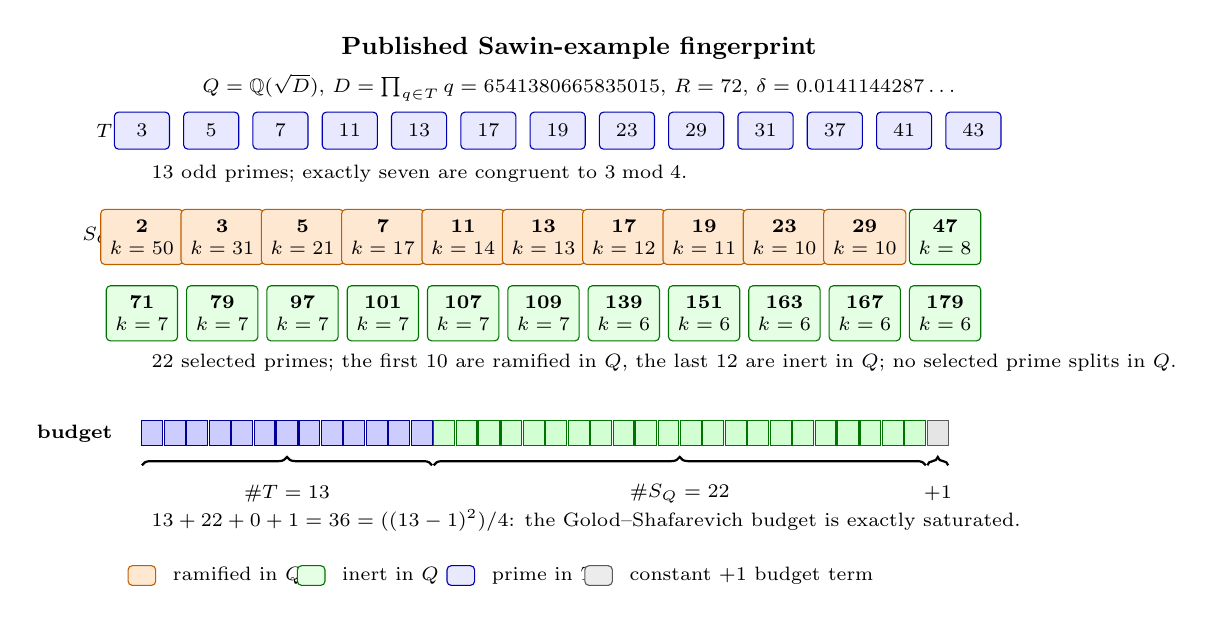
\begin{tikzpicture}[
  font=\scriptsize,
  tcell/.style={draw=blue!70!black, fill=blue!9, rounded corners=1.5pt, minimum width=0.70cm, minimum height=0.47cm, align=center},
  inertcell/.style={draw=green!45!black, fill=green!10, rounded corners=1.5pt, minimum width=0.90cm, minimum height=0.70cm, align=center},
  ramcell/.style={draw=orange!75!black, fill=orange!18, rounded corners=1.5pt, minimum width=0.90cm, minimum height=0.70cm, align=center},
  basecell/.style={draw=gray!70!black, fill=gray!15, rounded corners=1.5pt, minimum width=0.35cm, minimum height=0.25cm, align=center},
  note/.style={align=left, font=\scriptsize},
  lab/.style={font=\scriptsize\bfseries, anchor=east}
]

\node[font=\small\bfseries, align=center] at (5.55,1.05) {Published Sawin-example fingerprint};
\node[note, align=center] at (5.55,0.55) {$Q=\mathbb{Q}(\sqrt{D})$, $D=\prod_{q\in T}q=6541380665835015$, $R=72$, $\delta=0.0141144287\ldots$};

\node[lab] at (-0.25,0) {$T$};
\foreach \p [count=\i from 0] in {3,5,7,11,13,17,19,23,29,31,37,41,43} {
  \node[tcell] at (\i*0.88,0) {\p};
}
\node[note, anchor=west] at (0,-0.55) {13 odd primes; exactly seven are congruent to $3\bmod 4$.};

\node[lab] at (-0.25,-1.35) {$S_Q$};
\foreach \p/\k/\sty [count=\i from 0] in {2/50/ramcell,3/31/ramcell,5/21/ramcell,7/17/ramcell,11/14/ramcell,13/13/ramcell,17/12/ramcell,19/11/ramcell,23/10/ramcell,29/10/ramcell,47/8/inertcell} {
  \node[\sty] at (\i*1.02,-1.35) {\textbf{\p}\\$k=\k$};
}
\foreach \p/\k/\sty [count=\i from 0] in {71/7/inertcell,79/7/inertcell,97/7/inertcell,101/7/inertcell,107/7/inertcell,109/7/inertcell,139/6/inertcell,151/6/inertcell,163/6/inertcell,167/6/inertcell,179/6/inertcell} {
  \node[\sty] at (\i*1.02,-2.32) {\textbf{\p}\\$k=\k$};
}
\node[note, anchor=west] at (0,-2.95) {22 selected primes; the first 10 are ramified in $Q$, the last 12 are inert in $Q$; no selected prime splits in $Q$.};

\node[lab] at (-0.25,-3.85) {budget};
\foreach \i in {0,...,12} {\draw[draw=blue!60!black, fill=blue!20] ({0.285*\i},-4.00) rectangle ++(0.265,0.32);} 
\foreach \i in {13,...,34} {\draw[draw=green!45!black, fill=green!18] ({0.285*\i},-4.00) rectangle ++(0.265,0.32);} 
\draw[draw=gray!70!black, fill=gray!20] ({0.285*35},-4.00) rectangle ++(0.265,0.32);
\draw[decorate, decoration={brace, amplitude=3pt}, thick] (0,-4.25) -- ({0.285*13-0.02},-4.25) node[midway, yshift=-0.36cm] {$\#T=13$};
\draw[decorate, decoration={brace, amplitude=3pt}, thick] ({0.285*13},-4.25) -- ({0.285*35-0.02},-4.25) node[midway, yshift=-0.36cm] {$\#S_Q=22$};
\draw[decorate, decoration={brace, amplitude=3pt}, thick] ({0.285*35},-4.25) -- ({0.285*36-0.02},-4.25) node[midway, yshift=-0.36cm] {$+1$};
\node[note, anchor=west] at (0,-4.95) {$13+22+0+1=36=((13-1)^2)/4$: the Golod--Shafarevich budget is exactly saturated.};

\node[ramcell, minimum width=0.35cm, minimum height=0.25cm] at (0,-5.65) {};
\node[anchor=west] at (0.27,-5.65) {ramified in $Q$};
\node[inertcell, minimum width=0.35cm, minimum height=0.25cm] at (2.15,-5.65) {};
\node[anchor=west] at (2.42,-5.65) {inert in $Q$};
\node[tcell, minimum width=0.35cm, minimum height=0.25cm] at (4.05,-5.65) {};
\node[anchor=west] at (4.32,-5.65) {prime in $T$};
\node[basecell] at (5.80,-5.65) {};
\node[anchor=west] at (6.07,-5.65) {constant $+1$ budget term};
\end{tikzpicture}}
\caption{Parameter-level visualization of Sawin's published explicit example.  The figure is included here as a validation target for the verification pipeline and as a certificate-level illustration of the method.}
\label{fig:sawin-dashboard}
\end{figure}

\begin{figure}[htbp]
\centering
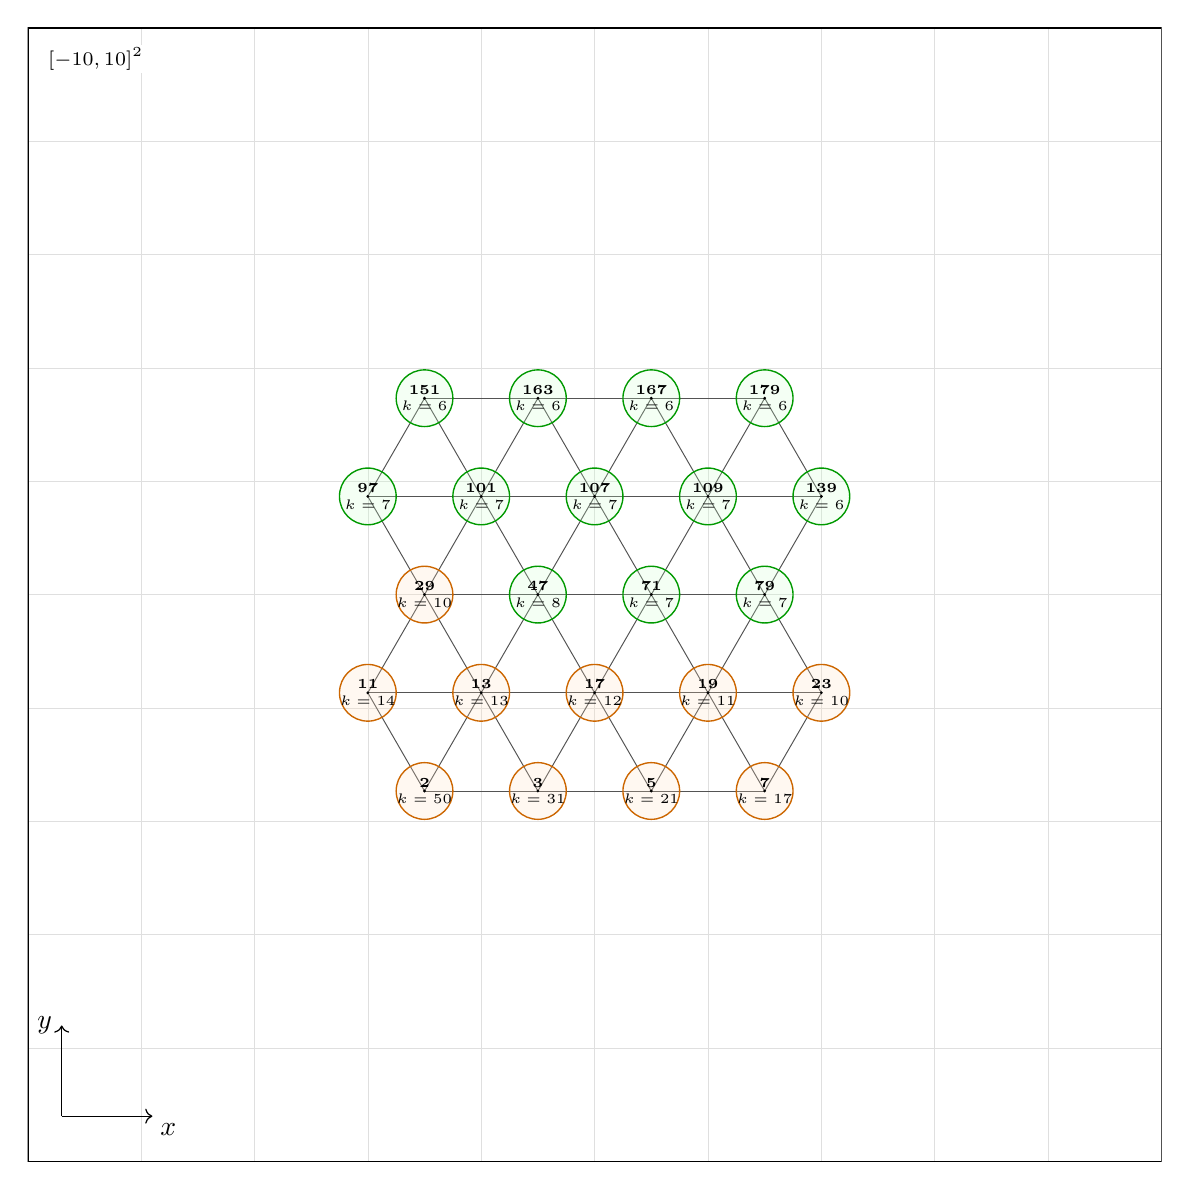
\begin{tikzpicture}[
  scale=0.72,
  contact/.style={draw=gray!65!black, line width=0.35pt},
  inertdisk/.style={draw=green!60!black, fill=green!20, fill opacity=0.22, line width=0.5pt},
  ramdisk/.style={draw=orange!80!black, fill=orange!25, fill opacity=0.22, line width=0.5pt},
  center/.style={circle, fill=black, inner sep=0.4pt},
  boundary/.style={draw=black, line width=0.7pt},
  gridline/.style={draw=gray!25, line width=0.2pt},
  plabel/.style={font=\tiny, align=center}
]
  \clip (-10,-10) rectangle (10,10);
  \foreach \g in {-10,-8,...,10} {\draw[gridline] (\g,-10) -- (\g,10);\draw[gridline] (-10,\g) -- (10,\g);} 
  \coordinate (a1) at (-3,-3.464);\coordinate (a2) at (-1,-3.464);\coordinate (a3) at (1,-3.464);\coordinate (a4) at (3,-3.464);
  \coordinate (b1) at (-4,-1.732);\coordinate (b2) at (-2,-1.732);\coordinate (b3) at (0,-1.732);\coordinate (b4) at (2,-1.732);\coordinate (b5) at (4,-1.732);
  \coordinate (c1) at (-3,0);\coordinate (c2) at (-1,0);\coordinate (c3) at (1,0);\coordinate (c4) at (3,0);
  \coordinate (d1) at (-4,1.732);\coordinate (d2) at (-2,1.732);\coordinate (d3) at (0,1.732);\coordinate (d4) at (2,1.732);\coordinate (d5) at (4,1.732);
  \coordinate (e1) at (-3,3.464);\coordinate (e2) at (-1,3.464);\coordinate (e3) at (1,3.464);\coordinate (e4) at (3,3.464);
  \draw[contact] (a1)--(a2);\draw[contact] (a2)--(a3);\draw[contact] (a3)--(a4);
  \draw[contact] (b1)--(b2);\draw[contact] (b2)--(b3);\draw[contact] (b3)--(b4);\draw[contact] (b4)--(b5);
  \draw[contact] (c1)--(c2);\draw[contact] (c2)--(c3);\draw[contact] (c3)--(c4);
  \draw[contact] (d1)--(d2);\draw[contact] (d2)--(d3);\draw[contact] (d3)--(d4);\draw[contact] (d4)--(d5);
  \draw[contact] (e1)--(e2);\draw[contact] (e2)--(e3);\draw[contact] (e3)--(e4);
  \draw[contact] (a1)--(b1);\draw[contact] (a1)--(b2);\draw[contact] (a2)--(b2);\draw[contact] (a2)--(b3);\draw[contact] (a3)--(b3);\draw[contact] (a3)--(b4);\draw[contact] (a4)--(b4);\draw[contact] (a4)--(b5);
  \draw[contact] (b1)--(c1);\draw[contact] (b2)--(c1);\draw[contact] (b2)--(c2);\draw[contact] (b3)--(c2);\draw[contact] (b3)--(c3);\draw[contact] (b4)--(c3);\draw[contact] (b4)--(c4);\draw[contact] (b5)--(c4);
  \draw[contact] (c1)--(d1);\draw[contact] (c1)--(d2);\draw[contact] (c2)--(d2);\draw[contact] (c2)--(d3);\draw[contact] (c3)--(d3);\draw[contact] (c3)--(d4);\draw[contact] (c4)--(d4);\draw[contact] (c4)--(d5);
  \draw[contact] (d1)--(e1);\draw[contact] (d2)--(e1);\draw[contact] (d2)--(e2);\draw[contact] (d3)--(e2);\draw[contact] (d3)--(e3);\draw[contact] (d4)--(e3);\draw[contact] (d4)--(e4);\draw[contact] (d5)--(e4);
  \foreach \name/\prime/\kk in {
    a1/2/50,a2/3/31,a3/5/21,a4/7/17,
    b1/11/14,b2/13/13,b3/17/12,b4/19/11,b5/23/10,
    c1/29/10
  } {
    \draw[ramdisk] (\name) circle[radius=0.5];
    \node[center] at (\name) {};
    \node[plabel] at (\name) {\textbf{\prime}\\$k=\kk$};
  }
  \foreach \name/\prime/\kk in {
    c2/47/8,c3/71/7,c4/79/7,
    d1/97/7,d2/101/7,d3/107/7,d4/109/7,d5/139/6,
    e1/151/6,e2/163/6,e3/167/6,e4/179/6
  } {
    \draw[inertdisk] (\name) circle[radius=0.5];
    \node[center] at (\name) {};
    \node[plabel] at (\name) {\textbf{\prime}\\$k=\kk$};
  }
  \draw[boundary] (-10,-10) rectangle (10,10);
  \draw[->, line width=0.45pt] (-9.4,-9.2) -- (-7.8,-9.2) node[below right=-1pt] {$x$};
  \draw[->, line width=0.45pt] (-9.4,-9.2) -- (-9.4,-7.6) node[left] {$y$};
  \node[font=\scriptsize, anchor=north west, fill=white, inner sep=1pt] at (-9.7,9.7) {$[-10,10]^2$};
\end{tikzpicture}
\caption{Schematic plane avatar for Sawin's published explicit example.  The 22 primes of $S_Q$ are attached to a finite contact patch in $[-10,10]^2$ using half-unit disks; orange marks ramified primes and green marks inert primes.  The figure serves only as a certificate-level illustration and validation aid.}
\label{fig:sawin-plane}
\end{figure}

\subsection*{Best-found candidate from the optimization procedure}



After the validation run above, the same pipeline was applied to the best candidate found by the optimization procedure.  That candidate is
\[
T=\{3,5,7,11,13,17,19,23,29,31,37,41,43\},
\]
with
\[
\begin{split}
S_Q=\{&2,3,47,71,79,97,101,107,109,139,151,163,167,179,\\
      &191,211,223,239,241,251,257,263\}.
\end{split}
\]
The chosen multiplicities are
\[
\begin{array}{c|rrrrrrrrrrr}
p&2&3&47&71&79&97&101&107&109&139&151\\
\hline
k(p)&47&29&7&6&6&6&6&6&6&5&5
\end{array}
\]
\[
\begin{array}{c|rrrrrrrrrrr}
p&163&167&179&191&211&223&239&241&251&257&263\\
\hline
k(p)&5&5&5&5&5&5&5&5&5&5&4
\end{array}
\]
and the grid-selected value is
\[
R=66.72240803.
\]

\subsection*{Visualization of the verified certificate}

Figure~\ref{fig:verified-candidate-dashboard} visualizes the optimized candidate at the parameter level.  It is not a drawing of the final Euclidean point configuration, whose construction is number-theoretic and asymptotic; rather, it shows the finite certificate data checked by the implementation: the prime set $T$, the selected primes $S_Q$, their multiplicities $k(p)$, and the exact saturation of the Golod--Shafarevich budget.

\begin{figure}[htbp]
\centering
\resizebox{0.98\linewidth}{!}{%
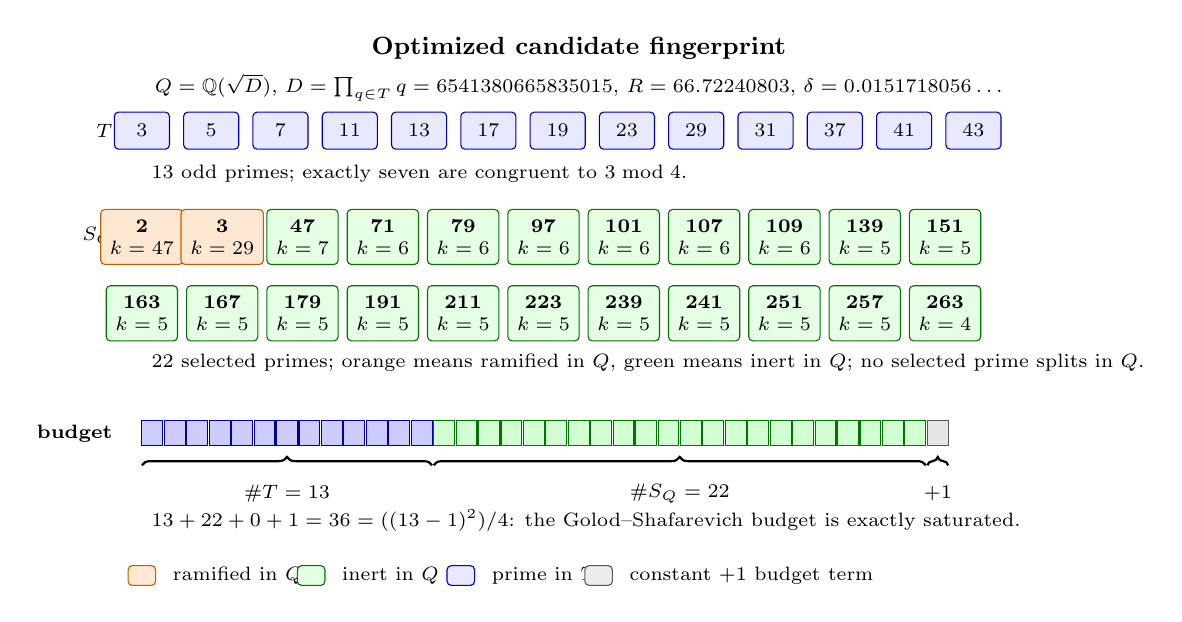
\begin{tikzpicture}[
  font=\scriptsize,
  tcell/.style={draw=blue!70!black, fill=blue!9, rounded corners=1.5pt, minimum width=0.70cm, minimum height=0.47cm, align=center},
  inertcell/.style={draw=green!45!black, fill=green!10, rounded corners=1.5pt, minimum width=0.90cm, minimum height=0.70cm, align=center},
  ramcell/.style={draw=orange!75!black, fill=orange!18, rounded corners=1.5pt, minimum width=0.90cm, minimum height=0.70cm, align=center},
  basecell/.style={draw=gray!70!black, fill=gray!15, rounded corners=1.5pt, minimum width=0.35cm, minimum height=0.25cm, align=center},
  note/.style={align=left, font=\scriptsize},
  lab/.style={font=\scriptsize\bfseries, anchor=east}
]

\node[font=\small\bfseries, align=center] at (5.55,1.05) {Optimized candidate fingerprint};
\node[note, align=center] at (5.55,0.55) {$Q=\mathbb{Q}(\sqrt{D})$, $D=\prod_{q\in T}q=6541380665835015$, $R=66.72240803$, $\delta=0.0151718056\ldots$};

% T row.
\node[lab] at (-0.25,0) {$T$};
\foreach \p [count=\i from 0] in {3,5,7,11,13,17,19,23,29,31,37,41,43} {
  \node[tcell] at (\i*0.88,0) {\p};
}
\node[note, anchor=west] at (0,-0.55) {13 odd primes; exactly seven are congruent to $3\bmod 4$.};

% S_Q rows.
\node[lab] at (-0.25,-1.35) {$S_Q$};
\foreach \p/\k/\sty [count=\i from 0] in {2/47/ramcell,3/29/ramcell,47/7/inertcell,71/6/inertcell,79/6/inertcell,97/6/inertcell,101/6/inertcell,107/6/inertcell,109/6/inertcell,139/5/inertcell,151/5/inertcell} {
  \node[\sty] at (\i*1.02,-1.35) {\textbf{\p}\\$k=\k$};
}
\foreach \p/\k/\sty [count=\i from 0] in {163/5/inertcell,167/5/inertcell,179/5/inertcell,191/5/inertcell,211/5/inertcell,223/5/inertcell,239/5/inertcell,241/5/inertcell,251/5/inertcell,257/5/inertcell,263/4/inertcell} {
  \node[\sty] at (\i*1.02,-2.32) {\textbf{\p}\\$k=\k$};
}
\node[note, anchor=west] at (0,-2.95) {22 selected primes; orange means ramified in $Q$, green means inert in $Q$; no selected prime splits in $Q$.};

% Budget bar.
\node[lab] at (-0.25,-3.85) {budget};
\foreach \i in {0,...,12} {
  \draw[draw=blue!60!black, fill=blue!20] ({0.285*\i},-4.00) rectangle ++(0.265,0.32);
}
\foreach \i in {13,...,34} {
  \draw[draw=green!45!black, fill=green!18] ({0.285*\i},-4.00) rectangle ++(0.265,0.32);
}
\draw[draw=gray!70!black, fill=gray!20] ({0.285*35},-4.00) rectangle ++(0.265,0.32);
\draw[decorate, decoration={brace, amplitude=3pt}, thick] (0,-4.25) -- ({0.285*13-0.02},-4.25) node[midway, yshift=-0.36cm] {$\#T=13$};
\draw[decorate, decoration={brace, amplitude=3pt}, thick] ({0.285*13},-4.25) -- ({0.285*35-0.02},-4.25) node[midway, yshift=-0.36cm] {$\#S_Q=22$};
\draw[decorate, decoration={brace, amplitude=3pt}, thick] ({0.285*35},-4.25) -- ({0.285*36-0.02},-4.25) node[midway, yshift=-0.36cm] {$+1$};
\node[note, anchor=west] at (0,-4.95) {$13+22+0+1=36=((13-1)^2)/4$: the Golod--Shafarevich budget is exactly saturated.};

% Legend.
\node[ramcell, minimum width=0.35cm, minimum height=0.25cm] at (0,-5.65) {};
\node[anchor=west] at (0.27,-5.65) {ramified in $Q$};
\node[inertcell, minimum width=0.35cm, minimum height=0.25cm] at (2.15,-5.65) {};
\node[anchor=west] at (2.42,-5.65) {inert in $Q$};
\node[tcell, minimum width=0.35cm, minimum height=0.25cm] at (4.05,-5.65) {};
\node[anchor=west] at (4.32,-5.65) {prime in $T$};
\node[basecell] at (5.80,-5.65) {};
\node[anchor=west] at (6.07,-5.65) {constant $+1$ budget term};
\end{tikzpicture}}
\caption{Parameter-level visualization of the optimized candidate in Appendix~\ref{app:verification}. The colored budget bar shows exact saturation of the side condition: 13 slots for $T$, 22 slots for $S_Q$, no split-prime penalty, and one constant slot.}
\label{fig:verified-candidate-dashboard}
\end{figure}

\subsection*{Plane visualization and its limitation}

Figure~\ref{fig:verified-candidate-plane} gives a plane drawing associated with the optimized certificate, but not a coordinate realization of the algebraic construction.  The 22 selected primes in $S_Q$ are attached as labels to the centers of a finite unit-disk contact patch inside the square $[-10,10]^2$.  The disks have radius $1$ and transparent interiors with solid boundaries; two centers are connected precisely when the corresponding disks touch.  This drawing carries the verified certificate labels, but it is not a plot of the actual algebraic point set promised by the theorem.

\begin{figure}[htbp]
\centering
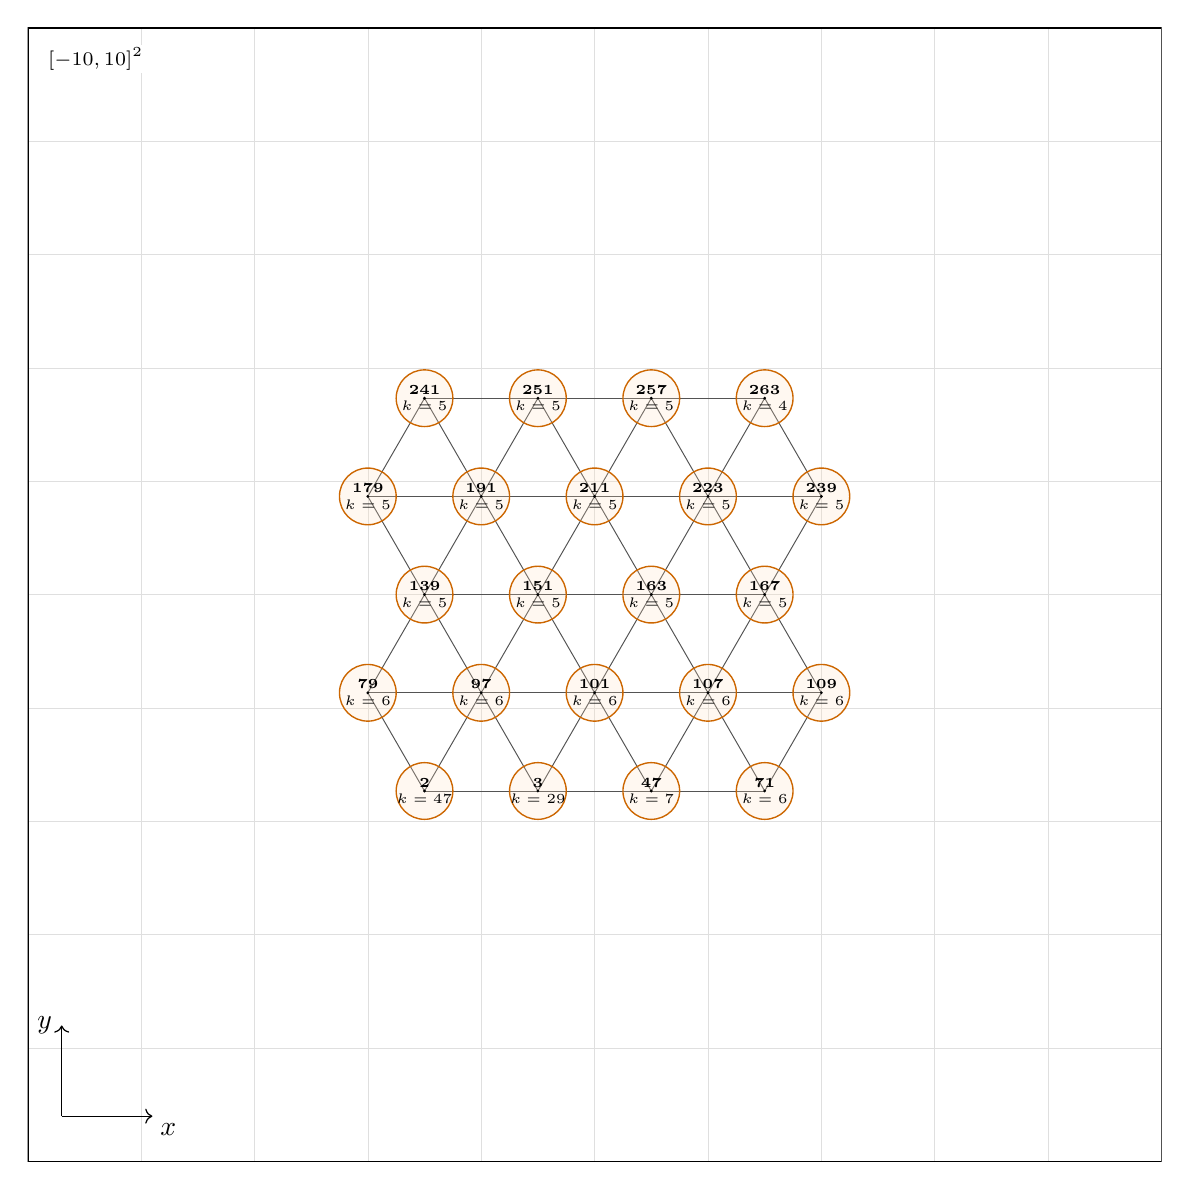
\begin{tikzpicture}[
  scale=0.72,
  contact/.style={draw=gray!65!black, line width=0.35pt},
  seldisk/.style={draw=orange!80!black, fill=orange!25, fill opacity=0.22, line width=0.5pt},
  center/.style={circle, fill=black, inner sep=0.4pt},
  boundary/.style={draw=black, line width=0.7pt},
  gridline/.style={draw=gray!25, line width=0.2pt},
  plabel/.style={font=\tiny, align=center}
]
  \clip (-10,-10) rectangle (10,10);
  \foreach \g in {-10,-8,...,10} {
    \draw[gridline] (\g,-10) -- (\g,10);
    \draw[gridline] (-10,\g) -- (10,\g);
  }
  \coordinate (a1) at (-3,-3.464);
  \coordinate (a2) at (-1,-3.464);
  \coordinate (a3) at (1,-3.464);
  \coordinate (a4) at (3,-3.464);
  \coordinate (b1) at (-4,-1.732);
  \coordinate (b2) at (-2,-1.732);
  \coordinate (b3) at (0,-1.732);
  \coordinate (b4) at (2,-1.732);
  \coordinate (b5) at (4,-1.732);
  \coordinate (c1) at (-3,0);
  \coordinate (c2) at (-1,0);
  \coordinate (c3) at (1,0);
  \coordinate (c4) at (3,0);
  \coordinate (d1) at (-4,1.732);
  \coordinate (d2) at (-2,1.732);
  \coordinate (d3) at (0,1.732);
  \coordinate (d4) at (2,1.732);
  \coordinate (d5) at (4,1.732);
  \coordinate (e1) at (-3,3.464);
  \coordinate (e2) at (-1,3.464);
  \coordinate (e3) at (1,3.464);
  \coordinate (e4) at (3,3.464);
  \draw[contact] (a1) -- (a2);\draw[contact] (a2) -- (a3);\draw[contact] (a3) -- (a4);
  \draw[contact] (b1) -- (b2);\draw[contact] (b2) -- (b3);\draw[contact] (b3) -- (b4);\draw[contact] (b4) -- (b5);
  \draw[contact] (c1) -- (c2);\draw[contact] (c2) -- (c3);\draw[contact] (c3) -- (c4);
  \draw[contact] (d1) -- (d2);\draw[contact] (d2) -- (d3);\draw[contact] (d3) -- (d4);\draw[contact] (d4) -- (d5);
  \draw[contact] (e1) -- (e2);\draw[contact] (e2) -- (e3);\draw[contact] (e3) -- (e4);
  \draw[contact] (a1) -- (b1);\draw[contact] (a1) -- (b2);\draw[contact] (a2) -- (b2);\draw[contact] (a2) -- (b3);\draw[contact] (a3) -- (b3);\draw[contact] (a3) -- (b4);\draw[contact] (a4) -- (b4);\draw[contact] (a4) -- (b5);
  \draw[contact] (b1) -- (c1);\draw[contact] (b2) -- (c1);\draw[contact] (b2) -- (c2);\draw[contact] (b3) -- (c2);\draw[contact] (b3) -- (c3);\draw[contact] (b4) -- (c3);\draw[contact] (b4) -- (c4);\draw[contact] (b5) -- (c4);
  \draw[contact] (c1) -- (d1);\draw[contact] (c1) -- (d2);\draw[contact] (c2) -- (d2);\draw[contact] (c2) -- (d3);\draw[contact] (c3) -- (d3);\draw[contact] (c3) -- (d4);\draw[contact] (c4) -- (d4);\draw[contact] (c4) -- (d5);
  \draw[contact] (d1) -- (e1);\draw[contact] (d2) -- (e1);\draw[contact] (d2) -- (e2);\draw[contact] (d3) -- (e2);\draw[contact] (d3) -- (e3);\draw[contact] (d4) -- (e3);\draw[contact] (d4) -- (e4);\draw[contact] (d5) -- (e4);
  \foreach \name/\prime/\kk in {
    a1/2/47,a2/3/29,a3/47/7,a4/71/6,
    b1/79/6,b2/97/6,b3/101/6,b4/107/6,b5/109/6,
    c1/139/5,c2/151/5,c3/163/5,c4/167/5,
    d1/179/5,d2/191/5,d3/211/5,d4/223/5,d5/239/5,
    e1/241/5,e2/251/5,e3/257/5,e4/263/4
  } {
    \draw[seldisk] (\name) circle[radius=0.5];
    \node[center] at (\name) {};
    \node[plabel] at (\name) {\textbf{\prime}\\$k=\kk$};
  }
  \draw[boundary] (-10,-10) rectangle (10,10);
  \draw[->, line width=0.45pt] (-9.4,-9.2) -- (-7.8,-9.2) node[below right=-1pt] {$x$};
  \draw[->, line width=0.45pt] (-9.4,-9.2) -- (-9.4,-7.6) node[left] {$y$};
  \node[font=\scriptsize, anchor=north west, fill=white, inner sep=1pt] at (-9.7,9.7) {$[-10,10]^2$};
\end{tikzpicture}
\caption{Schematic plane plot carrying the verified candidate labels from Appendix~\ref{app:verification}.  The 22 primes of $S_Q$ are attached to a finite unit-disk contact patch in $[-10,10]^2$; disks have radius $1/2$, transparent interiors, and solid boundaries, and edges connect pairs of touching disks.  This is not the algebraic point configuration promised by the theorem.}
\label{fig:verified-candidate-plane}
\end{figure}

\subsection*{Why the actual planar realization is not included}

A literal visualization of the part of the verified algebraic example lying in $[-10,10]^2$ would be mathematically natural, but the finite certificate studied here is not enough to produce such a coordinate plot.  The reason is that the verified candidate is a \emph{parameter certificate} for Sawin's explicit lower-bound criterion, not a finite coordinate list in $\mathbb{R}^2$.

The verification pipeline uses only finite arithmetic data:
\[
T,\qquad S_Q,\qquad k(p),\qquad R,
\]
together with exact Legendre-symbol checks and the Golod--Shafarevich budget inequality.  These checks are enough to test the hypotheses of the cited existence theorem and to evaluate the exponent in formula~\eqref{eq:delta-objective}.  They do not enumerate a number-field tower, produce a basis for the relevant algebraic objects, choose explicit embeddings, select a finite level of the asymptotic construction, or output planar coordinates.

Consequently, a literal plot of the verified configuration inside $[-10,10]^2$ would require an additional construction pipeline:
\begin{enumerate}
\item construct an explicit finite level of the required number-field/class-field object;
\item enumerate the algebraic elements corresponding to the chosen unit vectors;
\item choose and normalize the embeddings/projections used to place points in $\mathbb{R}^2$;
\item compute a finite point set and filter its coordinates to $[-10,10]^2$;
\item draw edges between pairs whose Euclidean distance is exactly $1$ after normalization.
\end{enumerate}
None of these coordinate-generation steps is implemented in the companion implementation or specified by the finite certificate alone.

This is why the appendix contains two different kinds of visualizations.  Figure~\ref{fig:verified-candidate-dashboard} is a genuine visualization of the verified finite certificate.  Figure~\ref{fig:verified-candidate-plane} is only a schematic contact drawing in the plane, included to show the unit-disk relation visually.  It should not be read as an isomorphic drawing of the actual unit-distance graph obtained from the algebraic construction.

\paragraph{Scope statement.}
This report therefore establishes a verified \emph{certificate check} relative to Sawin's criterion, but it does not construct or plot a concrete finite Euclidean point set realizing the candidate.  The verification is possible because the theorem reduces the lower-bound claim to finite arithmetic side conditions and a numerical exponent calculation.  The actual coordinate visualization is a separate and substantially larger computational number-theory task.


\subsection*{Attempted coordinate-generation pipeline}

The companion implementation also contains a recorded coordinate-generation attempt, which documents a deliberate effort to pass from the optimized certificate to coordinates.  The script loads the candidate $(T,S_Q,k,R)$, recomputes $D=\prod_{q\in T}q$, checks the splitting status of every selected prime in $S_Q$, verifies the Golod--Shafarevich budget, and recomputes the numerical exponent from formula~\eqref{eq:delta-objective}.  It then stops before coordinates are produced, with the status
\[
\texttt{BLOCKED\_BEFORE\_COORDINATES}.
\]
This is a mathematical obstruction rather than a plotting failure.

The reason is that Sawin's proof obtains planar point sets from lattices and projections attached to CM fields, with suitable fields supplied in arbitrarily large degree by a Golod--Shafarevich class-field-tower argument \cite{Sawin2026}.  The finite tuple $(T,S_Q,k,R)$ verifies the hypotheses and exponent of the criterion, but it does not specify one finite level of the tower by a defining polynomial, an integral basis, ideals, embeddings, and a bounded window.  Such data are necessary before one can enumerate points and then restrict them to $[-10,10]^2$.

More explicitly, a genuine coordinate realization would require:
\begin{enumerate}
\item an explicit finite level $L$ of the required tower, given by a computable basis or defining polynomial over $\mathbb Q$;
\item a certificate that $L/\mathbb Q(\sqrt D)$ has the required local and global properties;
\item the associated CM extension $K=L(i)$ and the relevant fractional ideals or algebraic elements used in the construction;
\item explicit complex embeddings and a lattice basis;
\item a normalization and bounded window from which a finite planar point set can be extracted;
\item an exact or certified numerical check of all unit-distance edges in the extracted finite set.
\end{enumerate}
Thus the certificate verification and the coordinate construction are different outputs.  The former is finite and is implemented here; the latter remains a substantially larger computational number-theory task.

\subsection*{Arithmetic checks}

Let
\[
D=\prod_{q\in T}q=6541380665835015,
\qquad
Q=\mathbb{Q}(\sqrt D).
\]
The set $T$ consists of odd primes and exactly seven of its elements are congruent to $3\pmod 4$, so the required parity condition is satisfied.  The verification checks, using exact integer arithmetic and Legendre-symbol computations, that every prime in $S_Q$ is either ramified or inert in $Q$; none is split.  Thus
\[
\#\{p\in S_Q:p\text{ splits in }Q\}=0.
\]
The Golod--Shafarevich budget side condition therefore becomes
\[
\#T+\#S_Q+\#\{p\in S_Q:p\text{ splits in }Q\}+1
=13+22+0+1=36,
\]
while
\[
\frac{(\#T-1)^2}{4}=\frac{12^2}{4}=36.
\]
Hence the budget is exactly saturated.

For admissibility in Sawin's Lemma~12, each $p\in S_Q$ must be congruent to $1\pmod 4$ or inert in $\mathbb{Q}(\sqrt q)$ for some $q\in T$.  The verification script found the following witnesses.

\begin{center}
\scriptsize
\begin{tabular}{rll}
\toprule
$p$ & status in $Q$ & admissibility witness \\
\midrule
2   & ramified & inert in $\mathbb{Q}(\sqrt5)$ \\
3   & ramified & inert in $\mathbb{Q}(\sqrt5)$ \\
47  & inert & inert in $\mathbb{Q}(\sqrt5)$ \\
71  & inert & inert in $\mathbb{Q}(\sqrt7)$ \\
79  & inert & inert in $\mathbb{Q}(\sqrt3)$ \\
97  & inert & $p\equiv1\pmod4$ \\
101 & inert & $p\equiv1\pmod4$ \\
107 & inert & inert in $\mathbb{Q}(\sqrt5)$ \\
109 & inert & $p\equiv1\pmod4$ \\
139 & inert & inert in $\mathbb{Q}(\sqrt3)$ \\
151 & inert & inert in $\mathbb{Q}(\sqrt3)$ \\
163 & inert & inert in $\mathbb{Q}(\sqrt3)$ \\
167 & inert & inert in $\mathbb{Q}(\sqrt5)$ \\
179 & inert & inert in $\mathbb{Q}(\sqrt7)$ \\
191 & inert & inert in $\mathbb{Q}(\sqrt7)$ \\
211 & inert & inert in $\mathbb{Q}(\sqrt3)$ \\
223 & inert & inert in $\mathbb{Q}(\sqrt3)$ \\
239 & inert & inert in $\mathbb{Q}(\sqrt7)$ \\
241 & inert & $p\equiv1\pmod4$ \\
251 & inert & inert in $\mathbb{Q}(\sqrt{11})$ \\
257 & inert & $p\equiv1\pmod4$ \\
263 & inert & inert in $\mathbb{Q}(\sqrt5)$ \\
\bottomrule
\end{tabular}
\end{center}

\subsection*{Numerical check}

Using 80-digit decimal arithmetic in the standard-library Python module \texttt{decimal}, the implementation evaluates formula~\eqref{eq:delta-objective} for the optimized candidate as follows:
\[
\begin{aligned}
\text{numerator}   &=4.3342249963460248\ldots,\\
\text{denominator} &=285.6762800674879\ldots,\\
\delta             &=0.01517180563721325\ldots .
\end{aligned}
\]
For the conservative target $0.015$, the margin is
\[
\text{numerator}-0.015\cdot \text{denominator}
=0.04908079533370595\ldots>0.
\]
The full 80-digit values are written to \texttt{verification\_attempt.txt}.
This margin is large compared with ordinary floating-point roundoff, although a publication-grade statement should still use formal interval arithmetic.

\begin{proposition}[Draft lower-bound consequence]
Assuming Sawin's explicit criterion is applied exactly as in \cite{Sawin2026}, the candidate above supports the clean bound
\[
  u(n)>n^{1.015}
\]
for arbitrarily large $n$.
\end{proposition}

\begin{remark}[Status of the claim]
The verification attempt passed all checks implemented in the self-contained implementation: primality, parity of $T$, admissibility of the primes in $S_Q$, absence of split primes in $Q$, exact saturation of the Golod--Shafarevich budget, positivity of all $k(p)$, $R>1$, and the numerical inequality $\delta>0.015$.  Thus the bundle does support a new clean lower bound relative to Sawin's published $n^{1.014}$ statement.  However, the sharper displayed value $1.0151718056\ldots$ should be treated as a candidate decimal until independently checked with interval arithmetic and reviewed by a human expert in the number-theoretic construction.
\end{remark}

\section*{Acknowledgements}

The author thanks Paul Erd\H{o}s for the original unit-distance problem; the OpenAI reasoning model and OpenAI team for the 2026 counterexample announcement and proof release; Noga Alon, Thomas F. Bloom, W. T. Gowers, Daniel Litt, Will Sawin, Arul Shankar, Jacob Tsimerman, Victor Wang, and Melanie Matchett Wood for the human-verified exposition and reflections; and Will Sawin for the explicit $n^{1.014}$ lower bound and for making the parameter-optimization question visible.  The report also acknowledges the earlier number-theoretic ideas signposted in the human-verified exposition, including work of Ellenberg--Venkatesh, Golod--Shafarevich, and Hajir--Maire--Ramakrishna.  Any remaining errors or overinterpretations are the author's responsibility.

\begin{thebibliography}{9}

\bibitem{Erdos1946}
P. Erd\H{o}s, ``On sets of distances of $n$ points,'' \emph{American Mathematical Monthly}, vol. 53, no. 5, pp. 248--250, 1946.

\bibitem{ST1983}
E. Szemer\'edi and W. T. Trotter, ``Extremal problems in discrete geometry,'' \emph{Combinatorica}, vol. 3, pp. 381--392, 1983.

\bibitem{SST1984}
J. Spencer, E. Szemer\'edi, and W. T. Trotter, ``Unit distances in the Euclidean plane,'' in \emph{Graph Theory and Combinatorics}, Academic Press, 1984, pp. 293--303.

\bibitem{OpenAI2026}
OpenAI, ``An OpenAI model has disproved a central conjecture in discrete geometry,'' May 20, 2026.  Available at \url{https://openai.com/index/model-disproves-discrete-geometry-conjecture/}.

\bibitem{AlonEtAl2026}
N. Alon, T. F. Bloom, W. T. Gowers, D. Litt, W. Sawin, A. Shankar, J. Tsimerman, V. Wang, and M. Matchett Wood, ``Remarks on the disproof of the unit distance conjecture,'' arXiv:2605.20695, 2026.  Available at \url{https://arxiv.org/abs/2605.20695}.

\bibitem{Sawin2026}
W. Sawin, ``An explicit lower bound for the unit distance problem,'' arXiv:2605.20579, 2026.  Available at \url{https://arxiv.org/abs/2605.20579}.

\end{thebibliography}

\end{document}
